\documentclass[12pt,a4paper]{article}
\usepackage[utf8]{inputenc}
\usepackage[german]{babel}
\usepackage[left=1.5cm,right=1.5cm,top=1.0cm,bottom=2.0cm]{geometry}
\usepackage{amsmath}
\usepackage{setspace}
\usepackage{array}
\setlength\extrarowheight{5pt}
\usepackage{multicol}
\usepackage{textcomp}
\usepackage{amsthm}
\usepackage{booktabs}
\usepackage{makecell}
\usepackage{hyperref}
\usepackage{framed}
\usepackage{chemmacros}
\usepackage{bbold}
\usepackage{mathrsfs}
\usepackage{amssymb}
\usepackage{graphicx}
\usepackage{tikz}
\usepackage[bottom]{footmisc}
\usetikzlibrary{arrows}
\usepackage{tikz-3dplot}
\usepackage{cancel}
\usepackage{wrapfig}
\DeclareMathOperator{\tr}{tr}
\usepackage{esint}
\usepackage{multicol}
\usepackage{tabularx}
\hypersetup{
    colorlinks,
    citecolor=black,
    filecolor=black,
    linkcolor=black,
    urlcolor=black
}
\let\vaccent=\v
\renewcommand{\v}[1]{\ensuremath{\mathbf{#1}}}
\newcommand{\iu}{{i\mkern1mu}}
\newcommand{\gv}[1]{\ensuremath{\mbox{\boldmath$ #1 $}}}
\newcommand{\abs}[1]{\left| #1 \right|}
\newcommand{\avg}[1]{\left< #1 \right>}
\let\underdot=\d
\renewcommand{\d}[2]{\frac{d #1}{d #2}}
\newcommand{\dd}[2]{\frac{d^2 #1}{d #2^2}}
\newcommand{\pd}[2]{\frac{\partial #1}{\partial #2}}
\newcommand{\pdd}[2]{\frac{\partial^2 #1}{\partial #2^2}}
\newcommand{\pdc}[3]{\left( \frac{\partial #1}{\partial #2}
 \right)_{#3}}
\newcommand{\ket}[1]{\left| #1 \right>}
\newcommand{\bra}[1]{\left< #1 \right|}
\newcommand{\braket}[2]{\left< #1 \vphantom{#2} \right|
 \left. #2 \vphantom{#1} \right>}
\newcommand{\matrixel}[3]{\left< #1 \vphantom{#2#3} \right|
 #2 \left| #3 \vphantom{#1#2} \right>}
\newcommand{\grad}[1]{\nabla #1}
\let\divsymb=\div
\renewcommand{\div}[1]{\nabla \cdot #1}
\newcommand{\rot}[1]{\nabla \times #1}
\let\baraccent=\=
\renewcommand{\=}[1]{\stackrel{#1}{=}}
\def\dbar{{\mathchar'26\mkern-12mu d}}
\newcommand{\rd}{\abs{\vec r - \vec r'}}
\newcommand{\ort}{\vec r}
\newcommand{\js}{\vec \jmath}
\newcommand{\erw}[1]{\langle #1 \rangle}
\newcommand{\eps}{\varepsilon}
\newcommand{\units}[2]{\frac{\text #1}{\text #2}}


\def\dbar{{\mathchar'26\mkern-12mu d}}
\newtheorem{satz}{Satz}
\theoremstyle{definition}
\newtheorem{dfn}{Definition}
\theoremstyle{remark}
\newtheorem*{rmk}{Bemerkung}
\thispagestyle{empty}
\title{Enchiridion Physica}
\author{Andreas Hemmetter}



\makeatletter
\def\@maketitle{
\raggedright
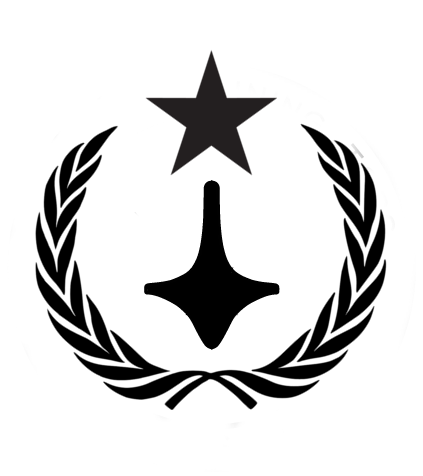
\includegraphics[width = 40mm]{pic/logofah.png}\\[8ex]
\begin{center}
{\Huge \bfseries \sffamily \@title }\\[4ex]
{\Large  \@author}\\[4ex]
\@date\\[8ex]

\vspace{100px}

\begin{framed}
\huge{
\begin{align*}
\delta \mathcal{S} &= \delta \int_{t_1}^{t_2} dt \mathscr{L} = 0 & \pd{F^{\alpha \beta}}{x^{\alpha}} &= \frac{4\pi}{c} j^{\beta}\\
S &= k_B \ln \Omega & i \hbar \pd{\psi}{t} &= \hat H \psi
\end{align*}}
\end{framed}


\end{center}}
\makeatother

\begin{document}

\maketitle
\thispagestyle{empty}
\newpage

\begin{multicols}{2}
\tableofcontents
\end{multicols}


\newpage
\setstretch{1.5}
\section{Mechanik}

\subsection[Kinematik des Massenpunktes]{Kinematik des Massenpunktes\let\thefootnote\relax\footnote{$g$: Fallbeschleunigung $[\frac{m}{s^2}]$, $c_W$: Luftreibungskoeffizient, $D$: Direktionsmoment $[Nm]$, $q$: elektrische Ladung $[C]$, $E$: elektrisches Feld $[\frac{V}{m}]$, $B$: magnetische Flussdichte $[Am]$, $\varepsilon_0$: elektrische Feldkonstante $[\frac{As}{Vm}]$}}

\begin{center}
\begin{minipage}[t]{.6\linewidth}
\vspace{0pt}
%\begin{center}
\begin{tabular}{ll}
schiefer Wurf & $y(x) = - \frac{g}{2 v_0^2 \cdot \cos^2(\alpha)} x^2 + \tan(\alpha) x + y_0$\\
Steigzeit & $T_s = \frac{v_0}{g} \sin(\alpha)$\\
Wurfhöhe & $h = \frac{v_0^2}{2g} \sin^2(\alpha)$\\
Wurfweite & $R = \frac{v_0^2}{g} \sin^2(\alpha)$\\
max. Wurfweite & $\alpha_{max} = \arcsin \frac{v_0}{\sqrt{2 v_0^2 + 2 g y_0}}$\\

\end{tabular}
%\end{center}
\end{minipage}%
\begin{minipage}[t]{.4\linewidth}
\vspace{0pt}
\centering
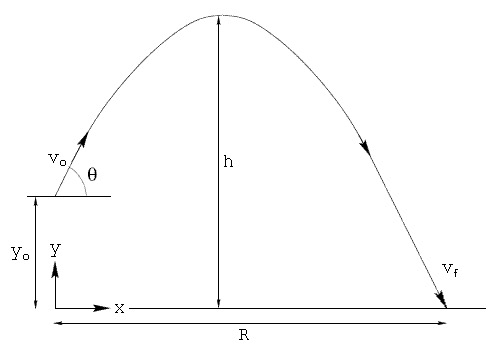
\includegraphics[width=\linewidth]{pic/schieferwurf.png}
\end{minipage}
\end{center}

\subsection{Dynamik des Massenpunktes}
\begin{center}
\begin{minipage}[t]{.5\linewidth}
\vspace{0pt}
\begin{tabular}{ll}
Luftreibung & $F_R = \frac{1}{2} c_W A \rho v^2$\\
Torsionsfederkraft & $F_D = -D \cdot \varphi$\\
Lorentzkraft & $\vec{F} = q(\vec{E} + \vec{v} \times \vec{B})$\\
Schubkraft Rakete & $F_S = - \frac{dm}{dt}u$\\
Radialkraft & $F_R = -m \omega^2 r = -m \frac{v^2}{r}$\\
Coulombkraft & $\vec{F}_{1,2} = \frac{q_1 \cdot q_2}{4 \pi \varepsilon_0 r_{12}^2} \cdot \frac{\vec{r_{12}}}{r_{12}}$\\
Corioliskraft & $F_C = 2m(\vec{v} \times \vec{\omega})$\\
Stokesreibung & $\vec{F} = - \alpha \dot{\vec{r}}$\\
Gleitreibung & $\vec{F} = -\mu F_{\perp} \hat{\dot{r}}$\\
Newtonreibung & $\vec{F} = -\beta v^2 \hat{\dot{r}}$\\
Kraft aus Potential & $\vec{F} = -\vec{\nabla}V$\\
\end{tabular}
\end{minipage}%
\begin{minipage}[t]{.5\linewidth}
\vspace{0pt}
\begin{framed}
1. Newton'sches Axiom: $\vec F = 0 \rightarrow \vec v = const.$\\
2. Newton'sches Axiom: $\vec{F} = m\vec{a} = \frac{d\vec{p}}{dt}$\\
3. Newton'sches Axiom: $\vec F_{A \rightarrow B} = - \vec F_{B \rightarrow A}$
\end{framed}

$\vec{F}(\vec{r})$ ist konservativ, falls:
\begin{itemize}
\itemsep-0.5em
\item $\vec{F} = \vec{F}(r)$
\item $\vec\nabla \times \vec{F} = 0$
\item $\exists V(\vec{r}): \vec{F} = -\vec\nabla V$
\item Arbeit $-\int_C d\vec{r} \cdot \vec{F}$ wegunabhängig
\item $-\oint_C d\vec{r} \cdot \vec{F} = 0$
\end{itemize}
$\vec{F}' = \vec{F} - m\dot{\vec{\omega}} \times \vec{r} - 2m\vec{\omega} \times \dot{\vec{\omega}}' - m\vec{\omega} \times (\vec{\omega} \times \vec{r})$
\end{minipage}
\end{center}


\subsection[Linearimpuls]{Linearimpuls\let\thefootnote\relax\footnote{$d$: Stoßparameter, $r$: Kugeldurchmesser, $I_{sp}$: spezifischer Impuls, $m_0$: Trockenmasse, $a$: durchschnittliche Halbachse, $\gamma$: Gravitationskonstante, $k$: Federkonstante $\units{N}{m}$, $D$: Federkonstante $[\frac{\text{N}}{\text{rad}}]$, $J_A$: Trägheitsmoment um andere Achse $[\text{kg} \text{m}^2]$}}
\begin{center}
\begin{minipage}[t]{.6\linewidth}
\vspace{0pt}
\begin{tabular}{ll}
Impuls & $\vec{p} = m \vec{v}$\\
elastischer Stoß Übertrag & $\Delta v = 2 \frac{m_1 v_1 + m_2 v_2}{m_1 + m_2}$\\
Stoßwinkel harte Kugeln & $\sin(\alpha) = \big(\frac{d}{2r}\big)$\\
Raketengleichung & $\Delta v = I_{sp} g \cdot \ln \frac{m}{m_0}$\\
Vis-Viva-Gleichung & $v^2 = \gamma M (\frac{2}{r} - \frac{1}{a})$\\
\end{tabular}
\end{minipage}%
\begin{minipage}[t]{.4\linewidth}
\vspace{0pt}
\centering
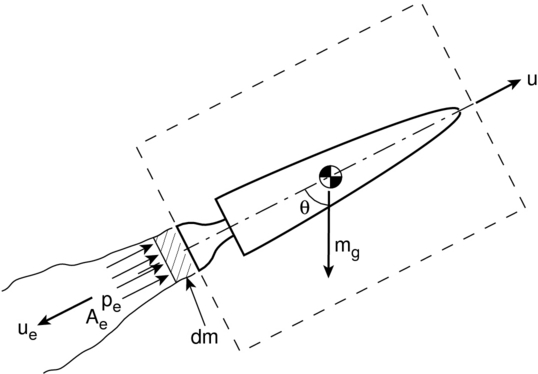
\includegraphics[width=\linewidth]{pic/rocket.jpg}
\end{minipage}
\end{center}


\subsection[Energie]{Energie\let\thefootnote\relax\footnote{}}

\begin{center}
\begin{minipage}[t]{.5\linewidth}
\vspace{0pt}
\begin{tabular}{ll}
Arbeit & $W = \vec{F} \cdot \vec{s} = -\int \vec{F} dx$\\
Arbeitselement & $\delta W = -\vec{F} \cdot d\vec{r}$\\
Gesamtenergie & $E = T + V$\\
Kinetische Energie & $E_{kin} = \frac{m}{2} v ^2$\\
Höhenenergie & $E_{pot} = mgh$\\
Spannenergie & $E_{spann} = \frac{1}{2}kx^2$\\
Reibungswärme Energie & $E_{R} = F_R s$\\
Thermische Energie & $E_{therm} = \frac{f}{2} k_B T$\\
Torsionsenergie & $E_{tors} = \frac{1}{2} D \varphi^2$\\
Rotationsenergie & $E_{rot} = \frac{1}{2} J_A \omega^2$\\
Leistung & $P = \frac{\Delta W}{\Delta t} = \vec{F} \cdot \vec{v}$\\
Leistung & $P = \d{W}{t}$\\
\end{tabular}
\end{minipage}%
\begin{minipage}[t]{.5\linewidth}
\vspace{0pt}
\centering
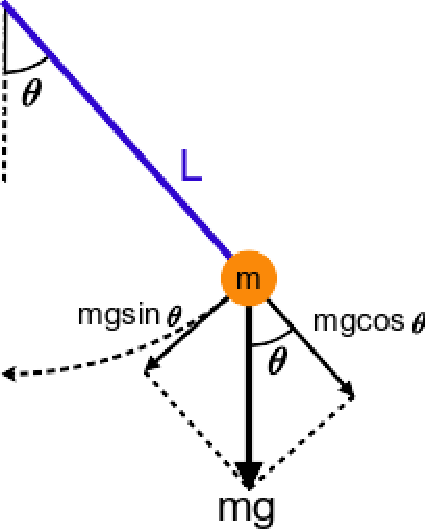
\includegraphics[width=0.7\linewidth]{pic/p22.pdf}
\end{minipage}
\end{center}


\subsection[Mechanik]{Mechanik\let\thefootnote\relax\footnote{$\delta$: Längenänderung [m], $A$: Angriffsfläche $[\text{m}^2]$, $\Delta_{max}$ maximale Deformation im Zentrum $[\text{m}]$, $\omega$: Kraft auf ganzen Balken $[\frac{\text{N}}{\text{m}}]$, $d_E$, $F_E$: Eingangsseite (effort), $d_R$, $F_R$: Ausgangsseite (reaction), pitch: Hubhöhe bei einer Umdrehung $[\text{m}]$, $U$: Umfang $[\text{m}]$, $N$: Anzahl Zähne, $t$: Drehmoment, $K$: Kompressionsmodul $[\frac{\text{N}}{\text{m}^2}]$, $G$: Schubmodul $[\frac{\text{N}}{\text{m}^2}]$, $\gamma$: Schubwinkel, $\nu$: Poissonzahl (Querkontraktionszahl)}}
\begin{center}
\begin{minipage}[t]{.55\linewidth}
\vspace{0pt}
\begin{tabular}{ll}
mech. Spannung & $\sigma = \frac{F}{A}$\\
Verformung & $\epsilon = \frac{\delta}{l_0}$\\
Young-Modulus & \makecell[l]{$E = \frac{\sigma}{\epsilon}$\\ $E = \frac{\sigma (F_2 - F_1) l_0}{(\delta_2 - \delta_1)A}$}\\
Deformation & $\delta = \frac{F l_0}{AE}$\\
Biegung Balken im Zentrum & $\Delta_{max} = \frac{F l^3}{48 E}$\\
Biegung Balken, gleichmäßig & $\Delta_{max} = \frac{5 \omega l^4}{384 E}$\\

Ideale Kraftersparnis & $IMA = \frac{d_E}{d_R}$\\
Wirkliche Kraftersparnis & $AMA = \frac{F_R}{F_E}$\\
Flaschenzug & $IMA = \frac{\text{gezogene Länge}}{\text{bewegte Länge}}$\\
Schiefe Ebene & $IMA = \frac{l}{h}$\\
Keil & $IMA = \frac{l}{h}$\\
Schraube & $IMA = \frac{U}{\text{pitch}}$\\
Zahnradsystem & $GR_{tot} = (\frac{B}{A})(\frac{D}{C})$\\
Statik-Bedingung & $\sum_i \vec{F}_i = 0, \sum_i \vec{M}_i = 0$\\
Kompressionsmodul & $K = -V \d{p}{V}$\\
Kompressionsmodul & $K = \frac{E}{3(1-2 \nu)}$\\
Kompressionskoeff. & $\kappa = \frac{1}{K}$\\
Schubmodul & $G = \frac{E}{2(1+\nu)}$\\
Schubspannung & $\tau = G \tan \gamma$\\
Poissonzahl & $\nu = \frac{\Delta d /d}{\Delta l / l}$\\
Übersetzungsverhältnis & $GR = \frac{N_{out}}{N_{in}} = \frac{d_{out}}{d_{in}} = \frac{\omega_{out}}{\omega_{in}} = \frac{t_{out}}{t_{in}}$\\
Flaschenzugverhältnis & $FR = \frac{d_{out}}{d_{in}} = \frac{\omega_{in}}{\omega_{out}} = \frac{t_{out}}{t_{in}}$
\end{tabular}
\end{minipage}%
\begin{minipage}[t]{.45\linewidth}
\vspace{0pt}

\begin{framed}
\centering Was man an Kraft spart, muss man an Weg zusetzen.
\end{framed}

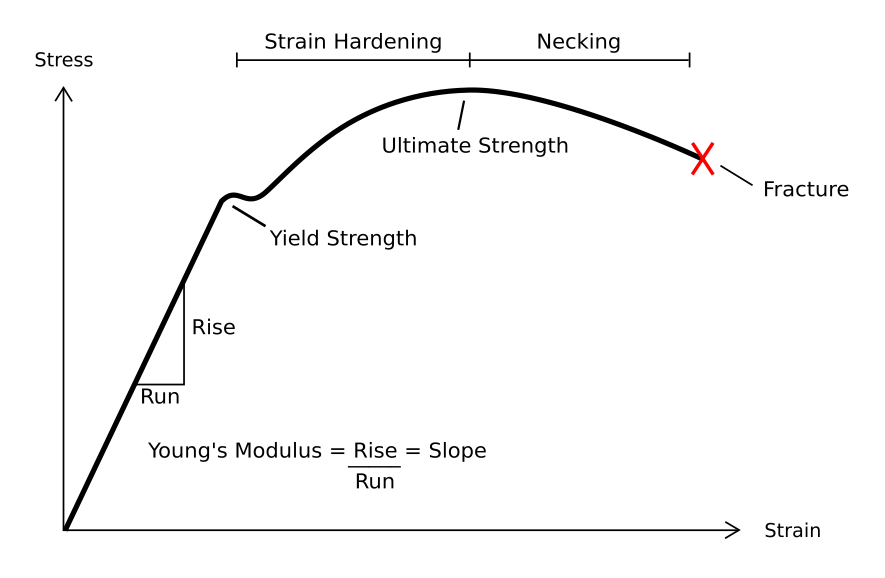
\includegraphics[width=\linewidth]{pic/stressstrain.png}
\vspace{20px}
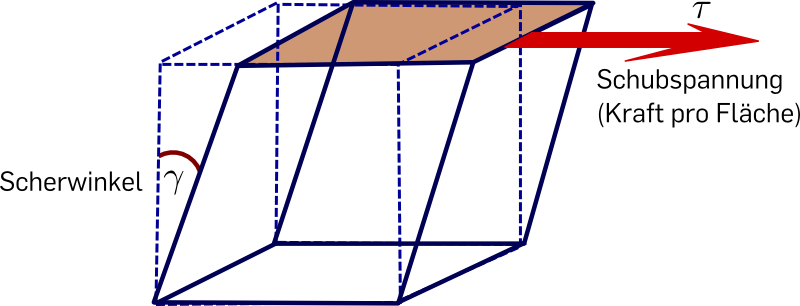
\includegraphics[width=0.7\linewidth]{pic/schubmodul.png}
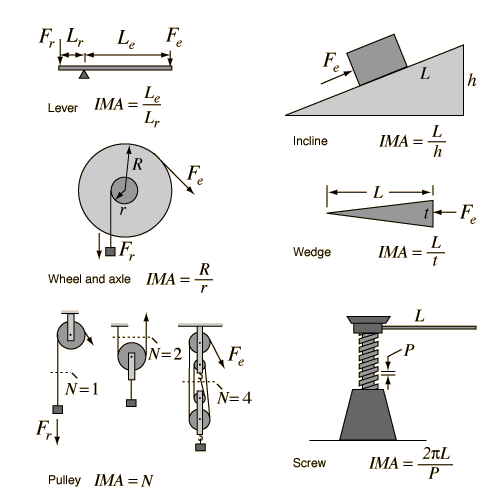
\includegraphics[width=\linewidth]{pic/simplemach.png}
\end{minipage}
\end{center}

\subsection[Drehungen]{Drehungen\let\thefootnote\relax\footnote{$r$: Radius, $T$: Periodenlänge, $\omega$: Winkelgeschwindigkeit, $\alpha$: Winkelbeschleunigung, $J$: Trägheitsmoment um Achse oder Schwerpunkt}}

\begin{center}
\begin{minipage}[t]{.6\linewidth}
\vspace{0pt}
\begin{tabular}{ll}
Bogenlängenelement & $\Delta s = r \cdot \Delta \varphi$\\
Winkelgrößen & $T = \frac{2 \pi}{\omega} = \frac{2 \pi r}{v} = \frac{1}{f}$\\
Tangentialgeschwindigkeit & $\vec{v} = \vec{\omega} \times \vec{r}$\\
Tangentialbeschleunigung & $\vec{\alpha_t} = \vec{\alpha} \times \vec{r}$\\
Radialbeschleunigung & $\vec{\alpha_r} = \omega^2 \cdot \vec{r} = \frac{v^2}{r}$\\
Gesamtdrehmoment & $J_S = \sum_i m_i r^2_i$\\
Steiner'scher Satz & $J_A = J_S + m s^2$\\
Massenschwerpunkt & $\vec{r}_M = \frac{\sum_i m_i \vec{r}_i}{\sum_i m_i}$\\
Bewegungsgleichung Drehung & $\varphi(t) = \frac{1}{2} \alpha t^2 + \omega_0 t + \varphi_0$\\
Drehmoment & $\vec{M} = \dot{\vec{L}} = \vec{r} \times \vec{F}$\\
Drehmoment (Betrag) & $M = F \cdot r \cdot \sin(\varphi) = J_A \ddot{\varphi}$\\
Drehimpuls & $\vec{L} = m \vec{r} \times \vec{v}$\\

\end{tabular}
\end{minipage}%
\begin{minipage}[t]{.4\linewidth}
\vspace{0pt}
\centering
\begin{tabular}{ll}
Trägheitsmoment & $J_S$\\
\midrule
Massepunkt & $mr^2$ \\
Vollzylinder & $\frac{1}{2}mr^2$ \\
Hohlkugel & $\frac{1}{2}m(r_2^2 - r_1^2)$ \\
Vollkugel & $\frac{2}{5}mr^2$ \\
Hohlkugel & $\frac{2}{3}mr^2$ \\
\makecell[l]{Stab um \\Schwerpunkt} & $\frac{1}{12}ml^2$ \\
Stab um Ende & $\frac{1}{3}ml^2$
\end{tabular}
\vspace{22.5pt}
\begin{flushleft}
\begin{tabular}{ll}
Translation & Rotation\\
\midrule
$\vec{a} = \dot{\vec{v}} = \ddot{\vec{x}}$ & $\vec{\alpha} = \dot{\vec{\omega}} = \ddot{\vec{\varphi}}$\\
$W = -\int F_x dx$ & $W = -\int M_A d \varphi$ \\
$P = F_xv_x$ & $P = M_A \omega$ \\
$\vec{p} = m \cdot \vec{v}$ & $L_A = J_A \omega$ \\
\end{tabular}
\end{flushleft}
\end{minipage}
\end{center}


\subsection[Zentralkraftfeld und Gravitation]{Zentralkraftfeld und Gravitation\let\thefootnote\relax\footnote{$A$: überstrichene Fläche, $L$: Drehimpulsbetrag, $\dot \phi$: Winkelgeschwindigkeit, $a$: große Halbachse, $M$: Masse des größeren Körpers, $\gamma$: Gravitationskonstante, $R$: Radius Erde, $h$: Höhe des Orbits, $e$: Exzentrizität, $\Theta$: Streuwinkel, $\Omega$: Raumwinkel, $\sigma$: Wirkungsquerschnitt}}
\begin{center}
\begin{minipage}[t]{.6\linewidth}
\vspace{0pt}
\begin{tabular}{ll}
Zentralkraft & $\vec{F} = f(\vec{r}, \dot{\vec{r}}, t) \cdot \hat{r}$\\
Flächenüberstreichung & $\Delta A = \frac{L}{2m} \Delta t$\\
2. Keplersches Gesetz & $\d{A}{t} = \frac{1}{2} r^2 \dot{\phi} = \frac{L}{2m} = const.$\\
3. Kepler'sches Gesetz & $\frac{T^2}{a^3} = \frac{4 \pi^2}{\gamma M} = const.$\\
Gravitationspotential & $V = - \frac{\gamma M m}{r}$\\
Gravitationskraft & $\vec{F}_{G12} = - \gamma \frac{m_1 \cdot m_2}{r_{12}^2} \cdot \frac{\vec{r_{12}}}{r_{12}}$\\
Gesamtenergie & $E = \frac{1}{2}mv^2 - \gamma \frac{m \cdot m_0}{r} = const.$\\
1. kosmische Geschwindigkeit & $v_1 = \sqrt{\frac{2 \gamma M}{R}}$\\
2. kosmische Geschwindigkeit & $v_2 = \sqrt{\frac{\gamma M}{R}}$\\
Umlaufzeit & $T_S(h) = 2 \pi \sqrt{\frac{R}{g}(1+\frac{h}{R})^3}$\\
Bahngeschwindigkeit & $v(h) = \sqrt{gR \Big(\frac{1}{1+\frac{h}{R}}\Big)}$\\
Ellipse & $e^2 = a^2-b^2$\\
numerische Exzentrität & $\varepsilon = \frac{e}{a}$\\
Rutherford &  $\Theta = 2 \arcsin \frac{1}{\sqrt{1 + \frac{4 E^2 s ^2 }{\alpha ^2}}}$\\
differentieller Wirkungsquerschnitt & $\d{\sigma}{\Omega} = \frac{\alpha ^2}{16E^2} \frac{1}{\sin^4 \frac{\Theta}{2}}$\\
totaler Wirkungsquerschnitt & $\sigma_{tot} = 2\pi \frac{\alpha^2}{16E^2} \int_0^{\pi} \frac{\sin \Theta d\Theta}{\sin^4 \frac{\Theta}{2}}$\\
\end{tabular}
\end{minipage}%
\begin{minipage}[t]{.4\linewidth}
\vspace{0pt}
\centering
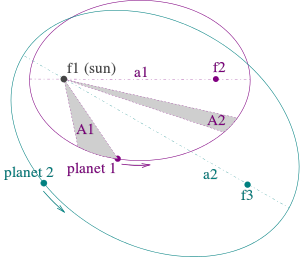
\includegraphics[width=.9\linewidth]{pic/kepler.png}
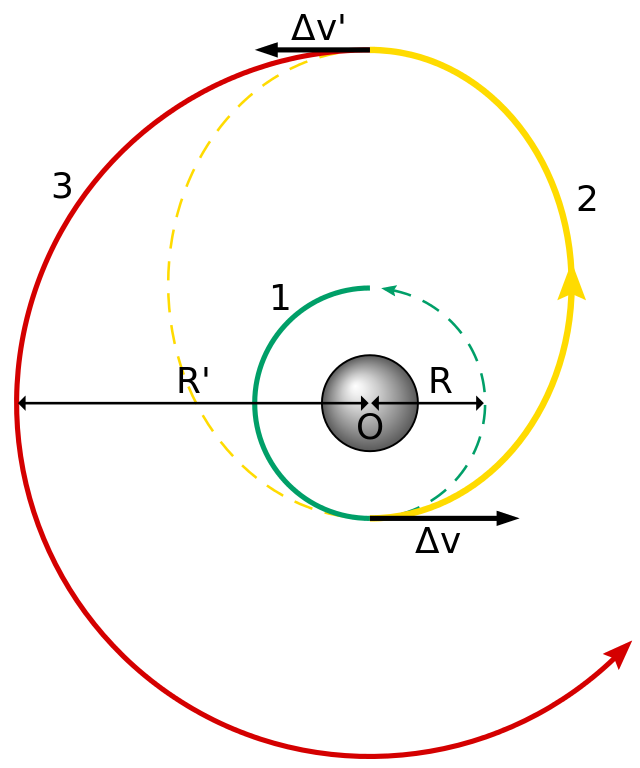
\includegraphics[width=.9\linewidth]{pic/hohmann.png}
\end{minipage}
\end{center}



\subsection[Mehrteilchensysteme]{Mehrteilchensysteme\let\thefootnote\relax\footnote{$\mu$: reduzierte Masse}}

\begin{center}
\begin{minipage}[t]{.5\linewidth}
\vspace{0pt}
\begin{tabular}{ll}
Bewegungsgleichung & $m_i \ddot{\vec{r}}_i = \vec{F}_i^{(ex)} + \sum_j \vec{F}_{ij}$\\
Reduzierte Masse & $\mu = \frac{m_1 m_2}{m_1 + m_2}$\\
Schwerpunktssatz & $M \ddot{\vec{R}} = \vec{F}^{(ex)}$\\
Schwerpunkt & $\vec{R} = \frac{m_1 \vec{r}_1 + m_2 \vec{r}_2}{m_1 + m_2}$\\
Impulssatz & $\dot{\vec{p}} = \vec{F}^{ex}$\\
Drehmoment & $\dot{\vec{L}} = \sum_i \vec{r}_i \times \vec{F}_i^{ex}$\\
kinetische Energie & $T = \sum_i \frac{1}{2} m_i \dot{\vec{r}}_i \cdot \dot{\vec{r}}_i$\\
konservative Kräfte & $\d{T}{t} = - \d{V}{t}$\\
Schwerpunktsbewegung & $\vec{R}(t) - \frac{\vec{p}}{M}t = \vec{R}(0) = const.$\\
Virialsatz & $2 \langle T \rangle = \langle \sum_i \vec{r}_i \cdot \nabla_i V \rangle$\\
Gesamtenergie & $\frac{M}{2} \dot{\vec{r}}_0^2 + \frac{1}{2} \sum_i m_i (\vec{\omega} \times \vec{r}_i)^2$\\
Drehimpuls & $\vec{L} = \overleftrightarrow{J}\vec{\omega}$\\
Rotationsenergie & $T_R = \frac{1}{2} \vec{\omega} \cdot \vec{L}$\\
Trägheitstensor & $J_{lm} = \int d^3 r \rho(\vec{r}) (\delta_{lm} \vec{r}^2 - x_l x_m)$\\
Drehmoment & $\vec{M} = \overleftrightarrow{J} \dot{\vec{\omega}} + \vec{\omega} \times \overleftrightarrow{J} \vec{\omega}$\\
Präzession & $\omega_P = \frac{m g r}{J \omega}$\\
\end{tabular}
\begin{framed}
Jede 3D-Transformation mit Fixpunkt kann als Rotation um eine Achse beschrieben werden. (Jeder Rotationsmatrix mit Fixpunkt hat Eigenwerte $\pm 1$.)\\
\centering\textsc{Euler'scher Satz}
\end{framed}
\end{minipage}%
\begin{minipage}[t]{.5\linewidth}
\vspace{0pt}
\centering
\begin{tabular}{ll}

\end{tabular}
\end{minipage}
\end{center}



\subsection[Relativitätstheorie]{Relativitätstheorie\let\thefootnote\relax\footnote{$\gamma$: Lorentzfaktor}}

\begin{center}
\begin{minipage}[t]{.45\linewidth}
\vspace{0pt}

\begin{framed}
$\gamma = \dfrac{1}{\sqrt{1 - \beta^2}} > 1$ und $\beta = \frac{v}{c} <1$
\end{framed}

\begin{tabular}{ll}
Galileo-Trafo & $\vec{r} = \vec{V}t + \vec{r}'$, $t = t'$\\
Zeitabl. Galileo-Trafo & $\d{}{t} = \Big(\d{}{t}\Big)' + \vec{\omega} \times$\\
Addition von Geschw. & $v_{tot} = \frac{v_1 + v_2}{1 + \frac{v_1 v_2}{c^2}} < c$\\
\end{tabular}

\begin{framed}
\begin{tabular}{ll}
$x\prime=\gamma(x - v_xt)$ & $x=\gamma(x\prime+v_xt)$ \\
$y\prime=y$ & $y=y\prime$\\
$t\prime=\gamma(t-v_x \frac{x}{c^2})$ & $t=\gamma(t\prime+v_x \frac{x\prime}{c^2})$\\
\end{tabular}
\end{framed}

\end{minipage}%
\begin{minipage}[t]{.5\linewidth}
\vspace{0pt}
\centering
\begin{tabular}{ll}
metrischer Tensor & $\begin{aligned} a^{\mu} &= g^{\mu \nu} a_{\nu}\\ a_{\mu} &= g_{\mu \nu} a^{\mu}\end{aligned}$\\
allg. Lorentztrafo & $\underline{x}_{\mu} = L_{\mu}^{\,\ \nu} x_{\nu}$ und $\underline{x}^{\mu} = L^{\mu}_{\,\ \nu} x^{\nu}$\\
kontravariant & {\small $(a^0, a^1, a^2, a^3) = (a^0, \vec{a})$}\\
kovariant &  {\small $(a_0, a_1, a_2, a_3) = (a^0, -\vec{a})$}\\
Skalarprodukt & $a_{\mu} b^{\mu} = a^{\mu}b_{\mu} = a^0b^0 - \vec{a} \cdot \vec{b}$\\
Betragsquadrat & $a_{\mu} a^{\mu} = (a^0)^2 - \vec{a} \cdot \vec{a}$\\
Vierervektorquadrat & $s^2 = c^2 t^2 - \vec{r}^2$\\
$\Delta s^2 > 0$: & zeitartig\\
$\Delta s^2 = 0$: & lichtartig\\
$\Delta s^2 < 0$: & raumartig\\
4-Geschw. & $u^0 = \gamma c$ und $\vec{u} = \gamma \vec{v}$\\
Geschw.quadrat & $u_{\mu} u^{\mu} = c^2$\\
4-Besch. & $a_{\mu} a^{\mu} = -\gamma^4 \Big[\gamma^2 \Big( \frac{\vec{v}}{c} \cdot \vec{a} \Big)^2 + \vec{a}^2 \Big]$\\
\end{tabular}

$g^{\mu \nu} =
\Bigg(\begin{smallmatrix}
1 & 0 & 0 & 0\\
0 & -1 & 0 & 0\\
0 & 0 & -1 & 0\\
0 & 0 & 0 & -1
\end{smallmatrix}\Bigg)$
und $L^{\mu}_{\,\ \nu} = \Bigg(\begin{smallmatrix}
\gamma & -\beta \gamma & 0 & 0\\
-\beta \gamma & \gamma & 0 & 0\\
0 & 0 & 1 & 0\\
0 & 0 & 0 & 1
\end{smallmatrix}\Bigg)$\\

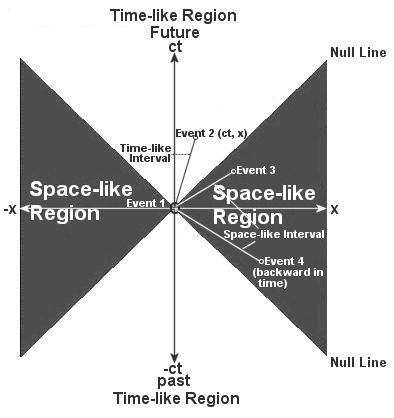
\includegraphics[width=.9\linewidth]{pic/minkowski.jpg}



\end{minipage}
\end{center}


%-----

\begin{center}
\begin{minipage}[t]{.5\linewidth}
\vspace{0pt}

\begin{tabular}{ll}

Gesamtenergie & $E^2 = m_0^2 c^4 + c^2p^2$\\
relativistische Energie & $E = \gamma m_0 c^2$\\
relativistischer Impuls & $p = \gamma m_0 v$\\
Zeitdilatation & $\Delta t = \gamma \Delta \tau$\\
Lorentzkontraktion & $l = \frac{l_0}{\gamma}$\\
Newton & $m \d{u^{\mu}}{\tau} = ma^{\mu} = K^{\mu}$\\
Kraft & $\vec{K} = \gamma \vec{F}$, $K^0 = \gamma \frac{\vec{F} \cdot \vec{v}}{c}$\\
Lagrange & $\d{}{\tau} \pd{\mathscr{L}}{u^{\mu}} - \pd{\mathscr{L}}{x^{\mu}} = 0$\\
\end{tabular}

\end{minipage}%
\begin{minipage}[t]{.5\linewidth}
\vspace{0pt}
\centering
\begin{tabular}{ll}
Divergenz & $\pd{x^{\mu}}{x^{\mu}} = 4$\\
Nabla & $\begin{aligned} &(\partial_0, \partial_1, \partial_2, \partial_3) = (\frac{1}{c} \pd{}{t}, \vec{\nabla})\\
&(\partial^0, \partial^1, \partial^2, \partial^3) = (\frac{1}{c} \pd{}{t}, -\vec{\nabla})\end{aligned}$\\
em. Feld & $\mathscr{L} = \frac{m}{2} v^2 + \frac{q}{c} \vec{v} \cdot \vec{A} - q \phi$\\
Vektorpotential & $(A_0, A_1, A_2, A_3) = (\phi, - \vec{A})$\\
Invarianten & $E^2 + H^2, \vec E \cdot \vec H$\\
Dopplereffekt & $\omega' = \omega_s (1-\beta)\gamma$\\
\end{tabular}

\begin{framed}
$E_y = \gamma (E_y' + \beta H_z')$, $H_y = \gamma (H_y' - \beta E_z')$\\
$E_z = \gamma (E_z' - \beta H_y')$, $H_z = \gamma (H_z' + \beta E_y')$\\
$\varphi = \gamma(\varphi' + \beta A_x')$, $A_x' = \gamma(A_x - \frac{\beta}{c} \varphi)$
\end{framed}

\end{minipage}
\end{center}


















\subsection[Fluide]{Fluide\let\thefootnote\relax\footnote{$A$: Querschnittsfläche Rohr, $I$: Volumenstrom, $g$: Fallbeschleunigung, $\eta$: dynamische Viskosität $[\text{Pa}~\text{s}]$, $\sigma$: Oberflächenspannung $[\frac{\text{N}}{\text{m}}]$, $h$: Steighöhe, $\varphi$: Winkel Oberfläche mit Gefäßwand}}

\begin{center}
\begin{minipage}[t]{.6\linewidth}
\vspace{0pt}
\begin{tabular}{ll}
Druck & $p = \frac{F}{A}$\\
Dichte & $\rho = \frac{m}{V}$\\
Bernoulli-Gesetz & $\overbrace{p_0}^\textrm{stat.} + \overbrace{\frac{1}{2}\rho v^2}^\textrm{dynam.} + \overbrace{\rho g y}^\textrm{pot.} = const.$\\
Kontinuitätsgleichung & $A_1 v_1 = A_2 v_2 = I = \frac{dV}{dt}$\\
Archimedisches Prinzip & $F_A = m_F g = \rho_F V_K g$\\
Volumenstrom Rohr & $\dot{V} = \frac{\pi r^4 \Delta p}{8 \eta l}$\\
Reibung Rohrströmung & $F_R = 8\pi\eta l \bar{v}$\\
laminarer Strömungswiderst. & $F_R = 6 \pi \eta r v$\\
Höhenformel & $p(z) = p_0 \cdot e^{-\frac{\rho_0 g z}{p_0}}$\\
Dichtebestimmung & $\rho_K = \rho_{F} \cdot \frac{|\vec{F_{G,L}}|}{|\vec{F_{G,L}}|-|\vec{F_{G,F}}|}$\\
Oberflächenspannung & $\sigma = \frac{dW}{dA} = \frac{F}{2l}$\\
Kapillareffekt & $h = \frac{2 \sigma \cos(\varphi)}{\rho r g}$\\
\end{tabular}
\end{minipage}%
\begin{minipage}[t]{.4\linewidth}
\vspace{0pt}
\centering
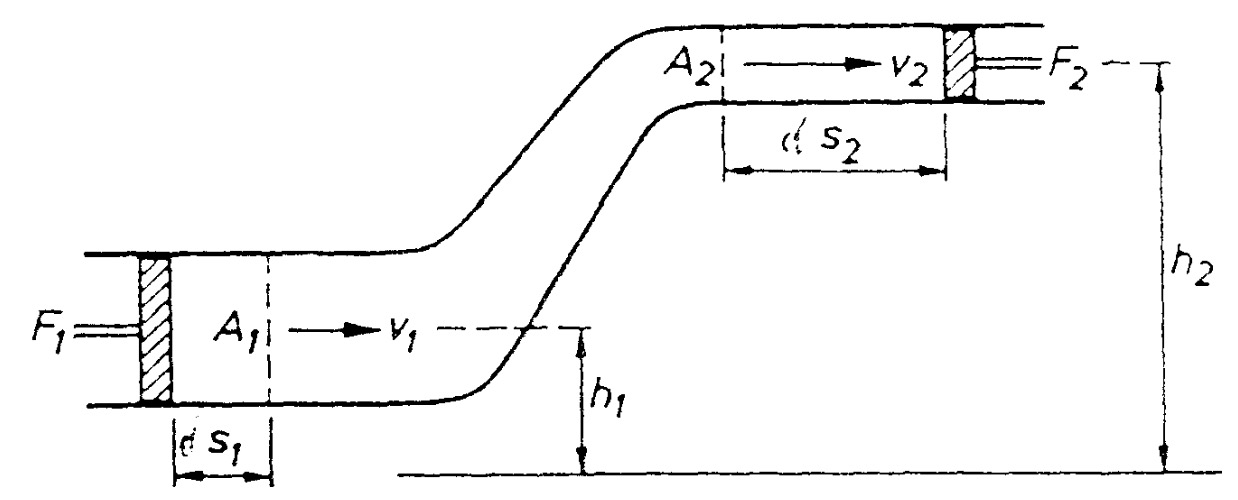
\includegraphics[width=\linewidth]{pic/bernoulli.png}
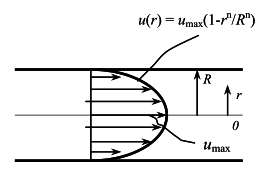
\includegraphics[width=\linewidth]{pic/rohr.png}
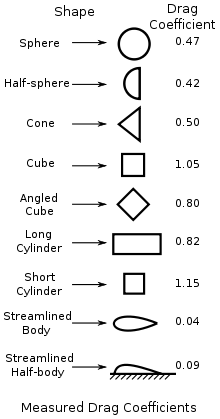
\includegraphics[width=\linewidth]{pic/luftcw.png}
\end{minipage}
\end{center}




\subsection[Schwingungen und Wellen]{Schwingungen und Wellen\let\thefootnote\relax\footnote{$\gamma$: Dämpfungsterm, $K$: Kompressionsmodul, $\rho$: Dichte, $P_S$: Schallleistung, $v$: Geschwindigkeit des Körpers, $c_s$: Schallgeschwindigkeit, $Ma$: Mach-Zahl, $b$: Reibungskoeffizient}}

\begin{center}
\begin{minipage}[t]{.5\linewidth}
\vspace{0pt}
$\ddot{x} + \underbrace{2 \gamma \dot{x}}_\text{Dämpfung} + \omega_0^2 x = \underbrace{\omega_0^2 x_0 \sin(\omega_A t)}_\text{Anregung}$\\
\begin{tabular}{ll}
harm. Schw. &  $x(t) = x_m \cos(\omega t + \alpha)$\\
Frequenz & $\omega = \sqrt{\omega_0^2 - \gamma^2}$\\
Schwebung & $\Delta \omega = \omega_1 - \omega_2$\\
Pot.näherung & $V(x) \cong V(x_0) + \frac{1}{2} \kappa (x-x_0)^2$\\
\end{tabular}
\end{minipage}%
\begin{minipage}[t]{.5\linewidth}
\vspace{0pt}
\begin{framed}
$$k = \frac{2 \pi}{\lambda}$$
$$c =  \frac{\omega}{k} = \lambda f = \frac{\lambda}{T}$$
\end{framed}

\begin{tabular}{ll}
Welle, 1D & $y(x,t) = y_m \sin(kx - \omega t)$\\
Gütefaktor & $Q = \frac{\omega_0}{\Delta \omega}$\\
Gesamtenergie & $E_{ges} = \frac{k}{2}A^2$\\
Abklingende Energie & $E = E_0 e^{-\frac{t}{\tau}}$\\
Transmissonskoeff. & $T = \frac{2v_2}{v_2 + v_1}$\\
Reflexionskoeff. & $R = \frac{v_2 - v_1}{v_2 + v_1}$\\
Absorptionskoeff. & $A = 1 - R - T$\\
Mittlere Leistung & $P_{gem} = \frac{1}{2}\mu v \omega^2 y_m^2$\\
Schallgeschwindigkeit & $v = \sqrt{\frac{K}{\rho}}$\\
Schall Druckdifferenz & $\Delta p_m = v \rho \omega s_m$\\
Schallintensität & $I = \frac{1}{2} \rho v \omega^2 s_m^2$, $I = \frac{P_S}{4 \pi r^2}$\\
sW, feste Enden & $f = \frac{v}{\lambda} = \frac{nv}{2l}$\\
sW, loses Ende & $f = \frac{v}{\lambda} = \frac{nv}{4l}$\\
Mach'scher Kegel (halb) & $\sin(\alpha) = \frac{c_S}{v} = \frac{1}{Ma}$\\
Reibung & $F_R = -b \dot{z}$, $\gamma = \frac{b}{2m}$\\
\end{tabular}
\end{minipage}
\end{center}

\newpage

\subsection[Lagrange]{Lagrange\let\thefootnote\relax\footnote{$N$: Teilchenzahl, $p$: Zwangsbedingungen, $S$: Wirkung}}

\begin{center}
\begin{minipage}[t]{.6\linewidth}
\vspace{0pt}
\begin{tabular}{ll}
skleronom (rheonom) & $\pd{f}{t} = (\neq) 0$\\
Freiheitsgrade & $S = 3N - p$\\
Bewegungsgleichung & $m_i \ddot{\vec{r}}_i = \vec{Z}_i + \vec{K}_i$\\
virtuelle Verrückung &  $\delta \vec{r}_i(t) = \vec{r}'_i(t) - \vec{r}_i(t)$\\
d'Alembert & $\sum_i (\vec{K}_i - \dot{\vec{p}}_i) \cdot \delta \vec{r}_i = 0$\\
generalisierte Kräfte & $Q_j = \sum_{i = 1}^N \vec{K}_i \cdot \pd{\vec{r}_i}{q_j}$\\
d'Alembert (gen.) & $\sum_{i = 1}^S \Big\{ \d{}{t} \pd{T}{\dot{q}_j} - \pd{T}{q_j} - Q_j \Big\} \delta q_j = 0$\\
holonom & $\d{}{t} \pd{T}{\dot{q}_j} - \pd{T}{q_j} = Q_j$\\
Gleichgewicht & $\sum_i Q_i \delta q_i = 0$\\
Lagrange-Gl. 2. Art & $\d{}{t} \pd{\mathscr{L}}{\dot{q}_j} - \pd{\mathscr{L}}{q_j} = 0$\\
L-F. em. Feld &  $\mathscr{L} = \frac{1}{2}m \dot{\vec{r}}^2 - q (\phi + \dot{\vec{r}} \cdot \vec{A})$\\
Euler'sche Gleichung & $\pd{f}{y} - \d{}{x}\pd{f}{y'} = 0$\\
konjugierter Impuls & $p_j = \pd{\mathscr{L}}{\dot{q}_j}$\\
zyklische Koord. & $\pd{\mathscr{L}}{q_j} = 0$\\
Hamilton-Fkt. & $H = \sum_j p_j \dot{q}_j - \mathscr{L}$\\
Tot. Zeitabl. H-F. & $\d{H}{t} = 0 = \pd{H}{t}$\\
Ray. Dissip.fkt. & $P = \sum_{i=1}^N \int_0^{v_i} dv'_i R_i(v'_i)$\\
Reibungskräfte & $Q_j^{(R)} = -\pd{P}{\dot{q}_j}$\\
Lagrange-Gl. 1. Art & $\d{}{t} \pd{\mathscr{L}}{\dot{q}_j} - \pd{\mathscr{L}}{q_j} = \sum_{\nu = 1}{k} \lambda_{\nu} a_{\nu j}$\\
\end{tabular}
\end{minipage}%
\begin{minipage}[t]{.4\linewidth}
\vspace{0pt}
%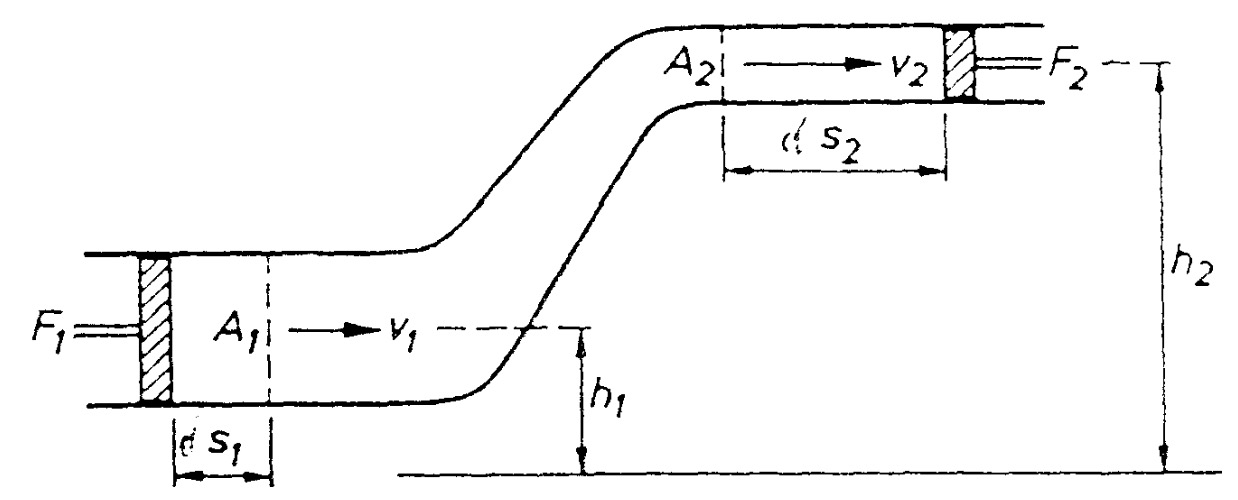
\includegraphics[width=\linewidth]{pic/bernoulli.png}
%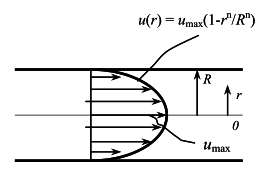
\includegraphics[width=\linewidth]{pic/rohr.png}

Lösungsschema Lagrange:
Zwangsbedingungen aufstellen $\Rightarrow$ Bewegung in generalisierten Koordinaten ausdrücken $\Rightarrow$ TF $\Rightarrow$ kinetische und potentielle Energie aufstellen $\Rightarrow$ Lagrange-Funktion $\mathscr{L}$ aufstellen $\Rightarrow$  Lagrange-Gleichung.

\begin{framed}\noindent\textbf{\textsc{Noether}-Theorem}: Zu jeder kontinuierlichen Symmetrie eines physikalischen Systems gehört eine Erhaltungsgröße.\\
Zeit homogen \dotfill $H = const.$,\\
Raum homogen \dotfill $\vec{p} = const.$,\\
Raum isotrop \dotfill $\vec{L} = const.$\end{framed}

\begin{framed}
\noindent
$$\mathbf{\delta \mathcal{S} =} \delta \int_{t_1}^{t_2} dt \mathscr{L}\mathbf{= 0}$$
\begin{center}\textsc{Weltformel}\end{center}
\end{framed}
\end{minipage}
\end{center}


\subsection[Hamilton]{Hamilton\let\thefootnote\relax\footnote{}}

\begin{minipage}[t]{.6\linewidth}
\vspace{0pt}

\begin{tabular}{ll}
Poissonkl. mit H & $\d{f}{t} = \{f, H\} + \pd{f}{t}$\\
Beliebige Poissonkl. & $\{f, g\}_{\vec{q}, \vec{p}} = \sum_{j=1}^S \Big( \pd{f}{q_j} \pd{g}{p_j} - \pd{f}{p_j} \pd{f}{q_j}\Big)$\\
$f$ Erhaltungsgröße & $\{f, H\} = 0$\\
$f$, $g$ erhalten & $\{f, g\}$ auch.\\
\end{tabular}

\begin{itemize}
\itemsep-0.5em
\item $\{f,g\}_{\vec{q}, \vec{p}} = \{f,g\}_{\vec{Q}, \vec{P}}$
\item $\{f, f\} = 0$
\item $\{f,g\} = -\{g, f\}$
\item $\{f+g, h\} = \{f,h\} + \{g, h\}$
\item $\{fg, h\} = f\{g,h\} + \{f,h\}g$
\item $\{\{f,g\}h\} + \{\{g,h\}, f\} + \{\{h,f\}, g\} = 0$
\end{itemize}

\begin{tabular}{l|l|l}
$F_1(\vec{q}, \vec{Q}, t)$ & $p_j = \pd{F_1}{q_j}$ & $P_j = - \pd{F_1}{Q_j}$\\
$F_2(\vec{q}, \vec{P}, t)$ & $p_j = -\pd{F_2}{q_j}$ & $Q_j = \pd{F_2}{P_j}$\\
$F_3(\vec{p}, \vec{Q}, t)$ & $q_j = -\pd{F_3}{p_j}$ & $P_j = - \pd{F_3}{Q_j}$\\
$F_4(\vec{p}, \vec{P}, t)$ & $q_j = -\pd{F_4}{p_j}$ & $Q_j = \pd{F_4}{P_j}$\\
\end{tabular}

\end{minipage}%
\begin{minipage}[t]{.4\linewidth}
\vspace{0pt}
Schema Hamilton: $q_j$ $\Rightarrow$  TF $\Rightarrow$  KE+PE $\Rightarrow$  $p_j$ $\Rightarrow$  auflösen nach $\dot{q}_j$ $\Rightarrow$  $\mathscr{L}$ $\Rightarrow$  Legendre $\Rightarrow$  KG $\Rightarrow$  $\int$

\begin{framed}
\begin{center}
$\begin{aligned}
\{q_i, q_j\} &= 0 \quad\\
\{p_i, p_j\} &= 0\\
\{q_i, p_j\} &= \delta_{ij}
\end{aligned}$\\
fund. Poissonklammern
\end{center}
\end{framed}

Phasentransformation ist kanonisch im weiteren Sinne, wenn:
\begin{itemize}
\itemsep-0.5em
\item $\forall H$ $\exists \tilde H$: $\vec{Q}, \vec{P}$ erfüllen mit $\tilde H$ die kanonischen Gleichungen.
\item $\delta \displaystyle\int_{t_1}^{t_2} dt \Big( \sum_j P_j \dot{Q}_j - \tilde H \Big)= 0$
\item $\sum_j p_j \dot{q}_j - H = c \Big( \sum_j P_j \dot{Q}_j - \tilde H \Big) + \d{F_1}{t}$
\item fund. Poissonklammern erfüllt
\end{itemize}
\end{minipage}

\noindent\begin{tabular}{ll}
Legendre 1 & $g(u) = f(x) -ux = f(x) - x \d{f}{x}$\\
Legendre 2 & $g(x,v) = f(x,y) - vy = f(x,y) - y (\pd{f}{y})_x$\\
Legendre H & $H = p\dot{q} - L = p \dot{q}^\star-\mathscr{L}^\star$\\
Liouville'scher Satz & $\d{\rho}{t} = 0$\\
\end{tabular}

\newpage
\section{Statistik}

\begin{framed}
$$n! \sim \sqrt{2\pi n} \big(\frac{n}{e}\big)^n$$
$$\ln(n!) = n \ln(n) - n$$
\centering\textsc{Stirling-Formel}
\end{framed}

\subsection[Wahrscheinlichkeitsverteilungen]{Wahrscheinlichkeitsverteilungen\let\thefootnote\relax\footnote{}}

\begin{tabular}{ll}
Wahrscheinlichkeit für Ereignis i & $p_i = \lim_{N \rightarrow \infty} \frac{N_i}{N}$\\
Realitätsbedingung & $\sum_i p_i = 1$\\
Addition von Wahrscheinlichkeiten & $P(i \lor j) = P_{i+j} = P_i + P_j$\\
Multiplikation von Wahrscheinlichkeiten & $P(i \land j) = P_{ij} = P_i \cdot P_j$\\
Charakteristische Funktion & $\varphi (k) = \int \exp(ikx) w(x) dx$\\
r-tes Moment aus charakt. Funktion & $\bar{x^r} = (-i)^r \frac{\text{d}^r}{\text{d}k^r} \varphi(k)|_{k=0}$\\
Binomialkoeffizienten & ${N \choose n} = \frac{N!}{(N-n)! n!}$\\
Gesetz der großen Zahlen & $\frac{\Delta A}{\bar A} \longrightarrow 0$\\
\end{tabular}

\noindent\begin{tabular}{lll}
\toprule
 & diskrete Verteilung & kontinuierliche Verteilung\\
\midrule
Norm $1$ & $\sum_i p_i$ & $\int w(x) dx$\\
Mittelwert $\bar x$ & $\langle x \rangle = \sum_i x_i p_i$ & $\int x w(x) dx$\\
r-tes Moment $\bar {x^r}$ & $\sum_i x_i^r p_i \neq {\bar x}^r$ & $\int x^r w(x) dx$\\
Varianz $(\Delta x)^2$ & $\bar{x^2} - \bar{x}^2$ & $\int x^2 w(x) dx - (\int x w(x) dx)^2$\\
\bottomrule
\end{tabular}

\noindent\begin{tabular}{llll}
\toprule
 & Binomalverteilung & Normalverteilung & Poissonverteilung\\
\midrule
Verteilung $P(n)$ & ${N \choose n} p^n q^{N-n}$ & $ \frac{1}{\sqrt{2\pi}\sigma} \exp{-\frac{(n-\bar{n})^2}{2\sigma^2}}$ & $\frac{\lambda^n}{n!} e^{-\lambda}$\\
Mittelwert $\bar{n}$ & $pN$ & $pN$ & $pN$\\
Varianz $(\Delta n)^2$ & $pqN$ & $pqN$ & $pN$\\
Gültigkeit & exakt & $\bar n = Np \gg 1 \text{ und } N - \bar n = Nq \gg 1$ & $p \ll  \text{ und } n \ll N$\\
\bottomrule
\end{tabular}

\subsection[Grundlagen]{Grundlagen\let\thefootnote\relax\footnote{}}

\noindent Ein \textbf{Mikrozustand} oder ein reiner Zustand $r$ beschreibt ein System vollständig, ohne jeglichen Informationsverlust.\\

\noindent Ein \textbf{Makrozustand} oder gemischter Zustand $\{P_r\}$ beschreibt ein System unvollständig und ist durch die Angabe der Wahrscheinlichkeiten $P_r$, mit denen bestimmte Mikrozustände $r$ eines Systems vorkommen können, festgelegt.\\

\noindent \textbf{Erreichbare} Mikrozustände sind alle die Zustände, die in einem gegebenen Makrozustand vorkommen können bzw. mit diesem verträglich sind. Sie müssen grundsätzlich abzählbar sein.\\

\begin{framed}\noindent In einem abgeschlossenen System ($E, V, N = $ const., d.h. mikrokanonisches Ensemble) im Gleichgewicht sind alle $\Omega$ erreichbaren Zustände $r$ gleichwahrscheinlich, d.h. es gilt $P_r = \frac{1}{\Omega}$ \end{framed}

\begin{flushleft}
\begin{tabular}{ll}
Planck-Zelle & $\tau = (2\pi \hbar)^f = h^f$\\
Gibbs-Faktor & $\frac{1}{N!}$\\
Ergodenhypothese & $\bar A^T = \bar A$\\
Statistische Entropie & $S = k \ln \Omega$\\
Volumen N-dimensionale Kugel & $V_N(R) = \frac{\pi^{N/2}}{()\frac{N}{2})!}R^N$\\
thermische Wellenlänge & $\lambda = \frac{h}{\sqrt{2\pi m k T}}$\\
\end{tabular}
\end{flushleft}

\subsection{Dichteoperator}


\begin{flushleft}
\begin{tabular}{ll}
Dichteoperator & $\hat \rho = \sum_r P_r \ket{\psi_r}\bra{\psi_r}$\\
\end{tabular}
\end{flushleft}

\subsection{Entropie}

\textbf{Fundamentalpostulat}: Im Gleichgewicht eines abgeschlossenen Systems ist die Entropie maximal.\\
\textbf{Extremalprinzip}: Im Gleichgewicht ist für alle Systeme die Entropie maximal: $\dbar S = 0$

\begin{flushleft}
\begin{tabular}{ll}
\toprule
Entropie & \\
\midrule
Thermodynamisch & $\dbar Q = T dS$\\
Statistisch & $S = k \ln \Omega(E, X)$\\
Informationstheoretisch & $S = - k \sum_i w_i \ln w_i$\\
\midrule
im Quantensystem & $S = -k \tr(\hat \rho \ln \hat \rho) = -k \langle \ln \hat \rho \rangle$\\
im klassischen System & $S = -k \int dq dp \rho(q, p) \ln [\tau \rho(q, p)]$\\
\bottomrule
\end{tabular}
\end{flushleft}

\subsection[Ensembles]{Ensembles\let\thefootnote\relax\footnote{}}

Ein \textbf{Ensemble} ist ein gedachtes Kollektiv vieler gleichartiger Systeme, in dem die zugänglichen Mikrozustände mit geforderten Nebenbedingung verträglich sind, mit bestimmten Wahrscheinlichkeiten vorkommen und den Makrozustand beschreiben. Im thermodynamischen Limit ($N \longrightarrow \infty$, $V \longrightarrow \infty$, $\frac{N}{V} = $ const.) sind alle Ensembles identisch und liefern die gleichen thermodynamischen Beziehungen.\\

\noindent \begin{tabular}{llllll}
\toprule
Ensemble & Konstanten & Variablen & $\rho_n$ & Zustandssumme & Dichteoperator $\hat \rho$\\
\midrule
Gen. kanonisches E. & & & & & \\
Mikrokanonisches E. & E, N, V & E, N, V & $\frac{1}{\Omega}$ & $\sum_{r: E-\Delta E \leq E_r \leq E} 1$ & $\frac{1}{\Omega} \sum_r \ket{\Phi_r}\bra{\Phi_r}$\\
Kanonisches E. & $\langle E \rangle$, N, V & T, N, V & $\frac{e^{-\beta E_r}}{Z}$ & $\sum_r e^{-\beta E_r} = \tr e^{-\beta \hat H}$ & $\frac{e^{-\beta \hat H}}{Z}$\\
Großkanonisches E. & $\erw{E}, \erw{N}, V$ &  T, $\mu$, V &  $\frac{e^{-\beta(E_r - \mu N_r)}}{Y}$ & $\sum_r e^{-\beta(E_r \mu N_r)}$ & $\frac{e^{-\beta(\hat H - \mu \hat N)}}{Y}$\\
\bottomrule
\end{tabular}


\newpage
\section{Thermodynamik}
\subsection[Grundbegriffe]{Grundbegriffe\let\thefootnote\relax\footnote{$R$: Gaskonstante $= 8.314 \frac{\text{J}}{\text{K}\text{mol}}$, $k_B$: Boltzmannkonstante, $N_A$: Avogadrozahl, $C_p, C_V$: Wärmekapazität bei konstantem Druck/Volumen}}

\begin{minipage}[t]{.7\linewidth}
\vspace{0pt}
\begin{tabular}{|c|c|c|c|}
\hline
 & $^{\circ}C$ & $^{\circ}K$ & $^{\circ}F$\\
\hline
$^{\circ}C$ & C & $C + 273,15$ & $\frac{9}{5}C + 32$\\
$^{\circ}K$ & $K - 273,15$ & K & $\frac{9}{5}(K - 273.15) + 32$\\
$^{\circ}F$ & $\frac{5}{9}(F - 32)$ & $\frac{5}{9}(F - 32) + 273,15$ & F\\
\hline
\end{tabular}
\end{minipage}%
\begin{minipage}[t]{.3\linewidth}
\vspace{0pt}
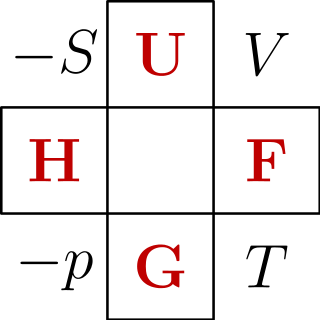
\includegraphics[width=0.7\linewidth]{pic/suv.png}
\end{minipage}
\end{center}

\begin{center}
\begin{minipage}[t]{.45\linewidth}
\vspace{0pt}

\begin{tabular}{ll}
ideales Gas & \makecell[l]{$\boxed{pV = nRT}$ \\$ = k_B N T $\\$= N_A n k_B T$}\\
reales Gas & \makecell[l]{$(p+\frac{an^2}{V^2} (V - bn)$\\$= nRT$}\\
Kompressionsarbeit & $W = -\int_{V_1}^{V_2} p dV$\\
Poisson-Konstante & $\gamma = C_p / C_V$\\
Gaskonstante & $R = C_p - C_V$\\
adiabatische Zst.gl. & $TV^{\gamma-1} = const.$\\
adiabatische Zst.gl. & $PV^{\gamma} = const.$\\
Wirkungsgrad & $\eta = \frac{\Delta W}{Q}$\\
Druck & $p = \frac{F_{\perp}}{A}$\\
Wärmestrom & $I = \frac{dQ}{dt} = \lambda A \frac{dT}{dx}$\\
Wärmedichte & $j = \frac{\dot{Q}}{A} = \lambda \frac{\Delta T}{l}$\\
Längenausdehnung & $dl = \alpha l dT$\\
Volumenausdehnung & $dV = \gamma V dT$\\
Thermische Energie & \makecell[l]{$E_{kin} = \frac{1}{2} m \bar{v}^2$\\ $= \frac{3}{2} k_B T$ {\scriptsize (pro Tlc.)} \\
$= \frac{1}{2} R T$ {\scriptsize (pro Mol)}}\\
\end{tabular}


\end{minipage}%
\begin{minipage}[t]{.55\linewidth}
\vspace{0pt}
\centering

\begin{tabular}{ll}
Wärmekapazität & d$Q = C dT$\\
Wärmemenge & $Q = C \cdot \Delta T$\\
innere Energie & $\Delta U = Q + W$\\
Entropieänderung & $\oint dS = 0$\\
reversibler Prozess & $dS_{rev} = \frac{dQ_{rev}}{T}$\\
WG Wärmemaschine & $\eta_C = \frac{|W|}{Q_w} = \frac{Q_w + Q_k}{Q_w} = \frac{T_w - T_k}{T_w}$\\
Kältemaschine & $C_L = \frac{Q_k}{W} = \frac{Q_k}{|Q_w| - Q_k} = \frac{T_k}{T_w - T_k}$ \\
Wärmepumpe & $C_L = \frac{|Q_w|}{W} = \frac{|Q_w|}{|Q_w| - Q_k} = \frac{T_w}{T_w - T_k}$ \\
Entropie & $\Delta S = C_V \cdot \ln \frac{T_2}{T_1} + nR \cdot \ln \frac{V_2}{V_1}$\\
Entropie & $S = k_B \cdot \ln P^{-1} = k_B \cdot \ln \Omega(M)$\\
\end{tabular}

%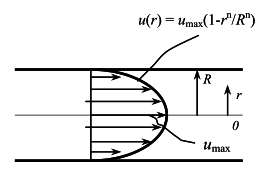
\includegraphics[width=\linewidth]{pic/rohr.png}
\end{minipage}
\end{center}

\subsection[Hauptsätze]{Hauptsätze\let\thefootnote\relax\footnote{}}
\subsubsection{0. Hauptsatz}
\begin{framed} \noindent Für jedes thermodynamische System existiert eine intensive Zustandsgröße, die Temperatur $T$. Ihre Gleichheit ist notwendige Voraussetzung für das thermische Gleichgewicht zweier Systeme.\end{framed}

\subsubsection{1. Hauptsatz}
\begin{framed} \noindent Für jedes thermodynamische System existiert eine extensive Zustandsgröße, die innere Energie E (=U). Sie ändert sich nur durch Austausch von Arbeit $A$ und Wärme $Q$ mit der Umgebung: $dU = \dbar A + \dbar Q$ \end{framed}

\begin{center}
\begin{minipage}[t]{.5\linewidth}
\vspace{0pt}
\begin{tabular}{ll}
Volumenänderung & $\dbar_V E = \dbar A = - p dV$\\
Impulsänderung & $\dbar_{\vec p}E = \vec v d\vec p$\\
Drehimpulsänderung & $\dbar_{\vec L}E = \vec \omega d\vec L$\\
Magnetisierungsänderung & $\dbar_{\vec M}E = \vec B d\vec M$\\
Ladungsänderung & $\dbar_Q E = \varphi dQ$\\
Polarisationsänderung & $\dbar_{\vec P}E = \vec E d\vec P$\\
Teilchenzahländerung & $\dbar_N E = \mu dN$\\
Gibbs-Form & $dE = \dbar Q = p dV + \mu dN$\\
\end{tabular}
\begin{tabular}{ll}
\toprule
Prozess & \\
\midrule
adiabatisch & $Q = 0, \Delta U = -W$ \\
isochor & $W = 0, \Delta U = Q$ \\
Kreisprozess & $\Delta U = 0, Q = W$ \\
freie Ausdeh. & $\Delta U = 0, Q = W$ \\
\bottomrule
\end{tabular}
\end{minipage}%
\begin{minipage}[t]{.5\linewidth}
\vspace{0pt}
\centering
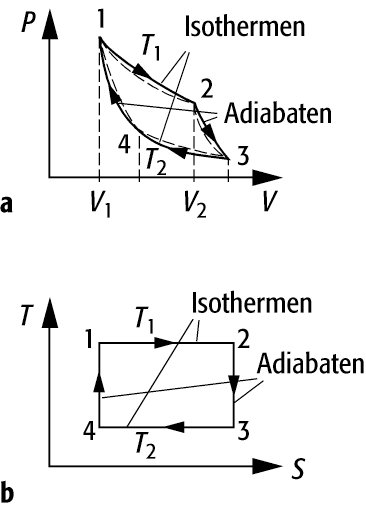
\includegraphics[width=0.7\linewidth]{pic/kreisprozess.jpg}
\end{minipage}
\end{center}

\newpage
\subsubsection{2. Hauptsatz}
\begin{framed} \noindent Für jedes thermodynamische Sysem existiert eine extensive Zustandsgröße, die Entropie $S$. Bei reversiblen Zustandsänderungen ändert sich die Entropie durch die mit der Umgebung ausgetauschten Wärmemenge. Bei irreversiblen Zustandsänderungen im abgeschlossenen System nimmt sie grundsätzlich zu: $dS \geq \frac{\dbar Q}{T}$ \end{framed}

\begin{framed}
\noindent \textbf{Sommerfeld}: Jedes thermodynamische System besitzt eine extensive Zustandsgröße $S$, die Entropie. Ihre Zunahme (Abnahme) $dS$ bei reversiblen Zustandsänderungen berechnet man, indem man die zugeführte (abgeführte) Wärmemenge $\dbar Q$ durch die bei dieser Gelegenheit definierten absoluten Temperatur dividiert.\\
\noindent \textbf{Clausius}: Es gibt keinen thermodynamischen Prozess, der nur darin besteht, dass Wärme von einem System mit Temperatur $T_1$ zu einem System mit Temperatur $T_2$ übertragen wird (mit $T_1 < T_2$).\\
\noindent \textbf{Kelvin}: Es gibt keinen thermodynamischen Prozess, der nur darin besteht, dass Wärme in Arbeit umgewandelt wird.\\
\noindent \textbf{Carnot}: Es gitb keine Wärmekraftmaschine, die effizienter als ein Carnot-Prozess ist.\\
\noindent \textbf{Planck}: Es ist unmöglich, eine periodisch arbeitende Maschine zu konstruieren, die nichts weiter bewirkt, als das Heben einer Last (d.h. Arbeit abgibt) und Abkühlung eines Wärmereservoirs.
\end{framed}

\subsubsection{3. Hauptsatz}

\begin{framed} \noindent Für jedes thermodynamische System nähert sich die Entropie $S$ ihrem kleinstmöglichen Wert am absoluten Nullpunkt unabhängig von Druck, Volumen, Aggregatszustand, etc. an.
Der absolute Nullpunkt der Temperatur ist durch keinen endlichen Prozess, sondern nur asymptotisch erreichbar.
$$S(T,X_i) \xrightarrow{T \rightarrow 0} S_0(X_i) = 0 \text{ und } \Big(\frac{\partial S(T,X_i)}{\partial(X_i)}\Big)_T \xrightarrow{T \rightarrow 0} 0$$\end{framed}

\subsection{Thermodynamische Potentiale}

\begin{tabular}{llll}
\toprule
Potential & Natürliche Var. & Grundgleichung & Euler-Gleichung\\
\midrule
Energie $U$ & S, V, N & $dE = T dS - p dV + \mu dN$ & $E = T \cdot S - p \cdot V + \mu \cdot N$\\
Freie Energie $F$ & T, V, N & $dF = -S dT - p dV + \mu dN$ & $F = -pV + \mu N$\\
Enthalpie $H$ & S, p, N & $dH = T dS + V dp + \mu dN$ & $H = TS + \mu N$\\
Freie Enthalpie $G$ & T, p, N & $dG = -S dT + V dp + \mu dN$ & $G = \mu N$\\
\makecell[l]{Gibbs'sche\\ Freie Energie $J$} & T, V, $\mu$ & $dJ = -S dT - p dV - N d\mu$ & $J = -pdV$\\
Entropie $S$ & E, V, N & $dS = \frac{1}{T} (dE + p dV - \mu dN)$ & $\frac{1}{T}(E + pV - \mu N)$\\
\bottomrule
\end{tabular}

\noindent \begin{tabular}{llll}
\toprule
Potential & & Zustandsgleichungen & \\
\midrule
Energie $U$ & $T = (\pd{E}{S})_{V, N}$ & $p = - (\pd{E}{V})_{S, N}$ & $\mu = (\pd{E}{N})_{S, V}$\\
Freie Energie $F$ & $S = -(\pd{F}{T})_{V, N}$ & $p = - (\pd{F}{V})_{T, N}$ & $\mu = (\pd{F}{N})_{T, V}$\\
Enthalpie $H$ & $T = (\pd{H}{S})_{p,N}$ & $V = (\pd{H}{p})_{S,N}$ & $\mu = (\pd{H}{N})_{S,p}$\\
Freie Enthalpie $G$ & $S = -(\pd{G}{T})_{p,N}$ & $V = (\pd{G}{p})_{T,N}$ & $\mu = (\pd{G}{N})_{T,p}$\\
Gibbs'sche Freie Energie $J$ & $S = -(\pd{J}{T})_{V, \mu}$ & $p = -(\pd{J}{V})_{T,\mu}$ & $N = -(\pd{J}{\mu})_{T,V}$\\
\bottomrule
\end{tabular}

\begin{framed}
$$S dT - V dp + N d\mu = 0$$
\centering\textsc{Gibbs-Duham-Relation}
\end{framed}

%\subsection{Potentiale und Ensembles}

%Kalorische Zustandsgleichung \dotfill $E(T,V,N) = - \pd{\ln Z}{\beta}$\\
%Thermische Zustandsgleichung \dotfill $p(T,V,N) = \frac{1}{\beta} \pd{\ln Z}{V}$\\
%Chemische Zustandsgleichung \dotfill $\mu(T,V,N) = - \frac{1}{\beta}\pd{\ln Z}{N}$\\

%\subsection{Ideales Quantengas}
%Symmetrie unter Vertauschung \dotfill $\ket{\psi(1,2)} = \pm \ket{\psi(2,1)}$ für Bosonen (+) und Fermionen (-)\\
%Besetzungszahlen Fermionen \dotfill $n_i = 0, 1$\\
%Besetzungszahlen Bosonen \dotfill $n_i = 0, 1, 2, ...$\\

%\noindent Großkanonische Zustandssumme für Bosonen \dotfill $Y_B(T,V,\mu) = \prod_{i=0}^{\infty} \frac{1}{1-e^{-\beta(\varepsilon_i-\mu)}}$\\
%Großkanonische Zustandssumme für Fermionen \dotfill $Y_F(T,V,\mu) = \prod_{i=0}^{\infty} (1+e^{-\beta(\varepsilon_i-\mu)})$\\

%\noindent Mittlere Besetzungszahl für Bosonen \dotfill $\bar{n_i}^B = \frac{1}{e^{\beta(\varepsilon_i-\mu)}-1}$\\
%Mittlere Besetzungszahl für Fermionen \dotfill $\bar{n_i}^F = \frac{1}{e^{\beta(\varepsilon_i-\mu)}+1}$\\

%\noindent $\mu$ kann für Fermionen jeden Wert annehmen\\
%$\mu < \varepsilon_0$ für Bosonen\\

%\noindent Mittlere Teilchenanzahl \dotfill $\erw{N} = \sum_i \bar n_i$\\
%Mittlere Energie \dotfill $\erw{E} = \sum_i \varepsilon_i \bar n_i$\\

%\noindent Teilchenanzahl Bosonen/Fermionen \dotfill $N = \sum_i \frac{1}{e^{\beta(\varepsilon_i - \mu)} \mp 1}$\\
%Thermische Zustandsgleichung Bosonen/Fermionen \dotfill $pV = \mp kT \sum_i \ln (1 \mp e^{-\beta(\varepsilon_i - \mu)})$\\
%Kalorische Zustandsgleichung Bosonen/Fermionen \dotfill $E = \sum_i \frac{\varepsilon_i}{e^{\beta(\varepsilon_i - \mu)} \mp 1}$\\

%\noindent Fugazität \dotfill  $z = e^{\beta \mu}$\\


%\subsection{Ideales Bose-Gas}

%Besetzungszahlen \dotfill $n(\varepsilon) = \frac{1}{e^{\frac{\varepsilon - \mu}{kT}} - 1}$\\
%Kondensatteilchen haben keine Energie und üben keinen Druck aus.\\

\newpage
\section{Elektrodynamik}

\subsection[Grundlagen]{Grundlagen\let\thefootnote\relax\footnote{}}

\begin{center}
\begin{minipage}[t]{.5\linewidth}
\vspace{0pt}
\noindent\begin{tabular}{ll}
Strom & $I = \dot{q} = \int_A \vec{\jmath} \cdot d\vec{A} = \frac{q U}{l \rho}$\\
Kontinuitätsgleichung & $\nabla \vec{\jmath} = -\pd{}{t} \rho$\\
Stromdichte & $\vec{\jmath} = \sigma_{el} \vec{E} = \rho \vec{v}$\\
Lorentzkraft & $\vec F = q(\vec E + \vec v \times \vec B)$\\
Lorentzkraftdichte & $\vec f = \rho \vec E + \vec \jmath \times \vec B$\\
\end{tabular}
\end{minipage}%
\begin{minipage}[t]{.5\linewidth}
\vspace{0pt}
\begin{tabular}{ll}
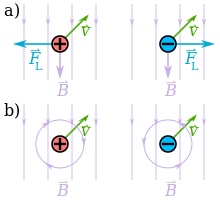
\includegraphics[width=\linewidth]{pic/lorentzkraft.png}
\end{tabular}
\end{minipage}
\end{center}

\subsection{Maxwell-Gleichungen}

\begin{framed}
\begin{align*}
\nabla & \cdot \vec E = \frac{\rho}{\varepsilon_0} & \nabla & \cdot \vec B = 0\\
\nabla &\times \vec E = - \pd{\vec{B}}{t} & \nabla & \times \vec B =  \mu_0 \vec \jmath + \frac{1}{c^2} \pd{\vec{E}}{t}
\end{align*}
\end{framed}

\begin{framed}
\begin{align*}
\oiint d\vec A \cdot \vec E &= \frac{1}{\eps_0}\iiint \rho dV & \oiint d\vec A \cdot \vec B &= 0\\
\oint d\vec r \cdot \vec E &= - \d{}{t} \iint d\vec A \cdot \vec{B} & \oint d\vec r \cdot \vec B &= \mu_0 \iint d\vec A \cdot \js + \frac{1}{c^2} \d{}{t} \iint d\vec A \cdot \vec{E}
\end{align*}
\end{framed}

\subsection[Elektrostatik]{Elektrostatik\let\thefootnote\relax\footnote{}}

\begin{center}
\begin{minipage}[t]{.5\linewidth}
\vspace{0pt}
\noindent\begin{tabular}{ll}
elektrostatische Kraft & $\vec F = q \vec{E}$\\
Ladungsdichte Punktladung & $\rho(\vec r) = Q \cdot \delta(\vec r - \vec r')$\\
Zwei Punktladungen & $\vec F = \frac{1}{4\pi \varepsilon_0} \frac{q_1 q_2}{r^2}\hat{e}_r$\\
\midrule
Dipolmoment & $\vec p = q \vec d$\\
Drehmoment E-Feld & $\vec{M} = \vec{p} \times \vec{E}$\\
Dipolmoment & $\vec p = \int dV \rho(\vec r) \vec r$\\
potentielle Energie Dipol & $W_{pot} = - \vec{p} \cdot \vec{E}$\\
Kraft auf Dipol &  $\vec{F} = \vec{p} \cdot \nabla \vec{E}$\\
induzierter Dipol & $\vec p = \alpha \vec E$\\
Polarisierbarkeit & $\alpha = \frac{3\varepsilon_0}{N} \frac{\varepsilon - 1}{\varepsilon + 2}$\\
Polarisation &  $\vec{P} = N \vec{p}_{ind} = \varepsilon_0 \chi \vec{E}_{D}$\\
Dielelektrizitätskonstante & $\varepsilon = 1 + \chi = 1 + \frac{3N \alpha}{3\varepsilon_0 - N\alpha}$\\
Polarisationsladungen &  $\nabla \cdot \vec{P} = - \rho_{pol}$\\
\midrule
Quadrupolmoment & $\overleftrightarrow D = \int dV \rho(\vec r) (3 \vec r \circ \vec r - \mathbb{1} r^2)$\\
Eigenschaften von $\overleftrightarrow D$: & \makecell[l]{$D_{ij} = D_{ji}$ \\ $\tr \overleftrightarrow D = \int dV (3 \vec r^2 - 3 \vec r^2) = 0$}\\
\midrule
Potential & $\vec E = -\nabla \varphi$\\
Poisson-Gleichung & $\Delta \varphi = -\frac{\rho}{\varepsilon_0}$\\
Laplace-Gleichung & $\Delta \varphi = 0$\\
Ladungsdichte & $\rho (\vec r, t) = \d{q}{V}$\\
E-Feld von $\rho$ & $E = \frac{1}{4\pi\varepsilon_0} \int_V \frac{\rho dV}{r^2}$\\
elektrisches Potential & $\varphi_{el} = \int_A \vec{E} \cdot dA$\\
Spannung  & $U = \int_{\varphi_1}^{\varphi_2} \vec{E} \cdot d\vec{s}$\\
Flächenladungsdichte & $\sigma = \frac{Q}{A}$\\
Oberflächenladung & $Q = \iint \sigma dA $\\
\end{tabular}
\end{minipage}%
\begin{minipage}[t]{.5\linewidth}
\vspace{0pt}
\begin{tabular}{ll}
\toprule

\end{tabular}
\end{minipage}
\end{center}

\begin{center}
\begin{minipage}[t]{.5\linewidth}
\vspace{0pt}
\noindent\begin{tabular}{ll}
Energiedichte (nur E) &  $w_{el} = \frac{1}{2} \varepsilon_0 E^2$\\
diel. Versch.dichte &  $\vec{D} = \varepsilon \varepsilon_0 \vec{E}_{Vak} + \vec{P}$\\
Energiedichte Dielektrika & $w_{el} = \frac{\varepsilon \varepsilon_0}{2} \cdot E^2 = \frac{1}{2} E \cdot D$\\
Ladung & $Q = C U$\\
E-Feld im Kond. &  $E = \frac{U}{d} = \frac{\sigma}{\varepsilon_0}$\\
Energie im Kond. & $W = \frac{1}{2} C U^2$\\
Plattenkondensator & $C = \varepsilon_0 \cdot \frac{A}{d}$\\
Kugelkondensator & $C = 4\pi\varepsilon_0 r$\\
Zylinderkondensator & $C = \frac{2\pi\varepsilon_0 l}{\ln(r_2/r_1)}$\\
\end{tabular}
\end{minipage}%
\begin{minipage}[t]{.5\linewidth}
\vspace{0pt}
\begin{tabular}{ll}

\end{tabular}
\end{minipage}
\end{center}


\noindent \begin{tabular}{lll}
\toprule
Geometrie & Potential $\phi$ & Feld $E$\\
\midrule
Punktladung & $\frac{1}{4\pi\varepsilon_0} \frac{q}{r}$ & $\frac{q}{4\pi \varepsilon_0 r^2}$\\
Unendliche Linienladung & $\frac{1}{2\pi\varepsilon_0} \lambda \ln\frac{r_B}{r}$ & $\frac{1}{4\pi\varepsilon_0} \frac{2\lambda}{r_{\perp}}$\\
Achse geladener Ring & $\frac{1}{4\pi\varepsilon_0} \frac{q}{\sqrt{z^2 + a^2 }}$ & $\frac{1}{4\pi\varepsilon_0} \frac{qz}{(z^2 +a^2)^{3/2}}$\\
Kreisscheibe & $\frac{1}{2 \varepsilon_0} \sigma \abs{z} (\sqrt{1+\frac{r_S^2}{z^2}}-1)$ & $\frac{\sigma}{2 \varepsilon_0} (1-(1+\frac{r^2}{z^2})^{-1})$\\
Unendliche Ebene & $\phi_0 - \frac{1}{2\varepsilon_0} \sigma \abs{x}$ & $\frac{\sigma}{2 \varepsilon_0}$\\
Kugelschale & $\frac{1}{4\pi\varepsilon_0} \frac{q}{r}$ & $\frac{1}{4\pi\varepsilon_0}\frac{q}{r^2}$\\
Dipol & $\frac{\vec p \cdot \vec r}{4\pi \varepsilon_0 r^3}$ & $\frac{1}{4\pi \varepsilon_0} \cdot \frac{3(\vec p \cdot \vec r)\vec r - \vec p r^2}{p^5}$\\
\bottomrule
\end{tabular}

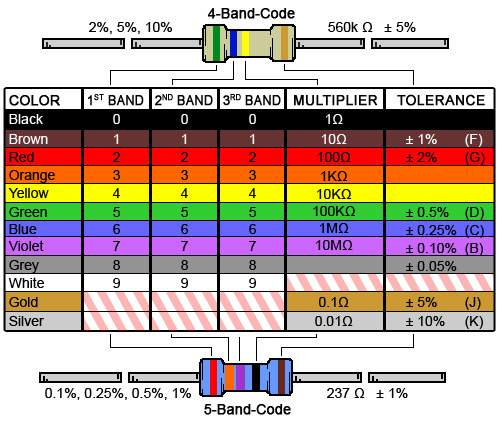
\includegraphics[width=0.6\textwidth]{pic/resistors.jpg}
\subsection[Gleichspannung]{Gleichspannung\let\thefootnote\relax\footnote{}}

\begin{center}
\begin{minipage}[t]{.5\linewidth}
\vspace{0pt}
\noindent\begin{tabular}{ll}
Ohm'sches Gesetz & $U = R \cdot I$\\
Knotensatz & $\sum_k I_k = 0$\\
Maschensatz & $\sum_k U_k = 0$\\
Leistung & $P = U I = I^2 R = \frac{U^2}{R}$\\
Widerstand & $R = \frac{l}{\sigma \cdot A} = \rho \frac{l}{A}$\\
Flächenwiderstand & $R_S = \frac{\rho}{d} = R \frac{B}{L}$\\
elektrische Arbeit & $W = q U = P t$\\
Wirkungsgrad & $\eta = \frac{P_{out}}{P_{in}}$\\
Leitwert & $G = 1 / \rho$\\
$R$ in Serie & $R_{ges} = \sum_i R_i$\\
$R$ parallel & $\frac{1}{R_{ges}} = \sum_i \frac{1}{R_i}$\\
$C$ in Serie & $\frac{1}{C_{ges}} = \sum_i \frac{1}{C_i}$\\
$C$ parallel & $C_{ges} = \sum_i C_i$\\
Temperaturabhängigkeit $R$ & $\Delta R = R_0 \alpha \Delta T$\\
Kapazitätsgleichung & $I_C = C \d{U_C}{t}$\\
Induktivitätsgleichung & $U_L = L \d{I_L}{t}$\\
\end{tabular}
\end{minipage}%
\begin{minipage}[t]{.5\linewidth}
\vspace{0pt}
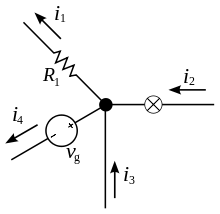
\includegraphics[width=\linewidth]{pic/knotenregel.png}
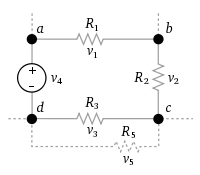
\includegraphics[width=\linewidth]{pic/maschenregel.png}
\end{minipage}
\end{center}
\newpage

\subsection[Wechselspannung]{Wechselspannung\let\thefootnote\relax\footnote{}}

\begin{center}
\begin{minipage}[t]{.5\linewidth}
\vspace{0pt}
\noindent\begin{tabular}{ll}
komplexe Spannung & $\hat U = U e^{i \varphi_n}$\\
effektive Spannung & $U_{eff} = \frac{U_m}{\sqrt{2}}$\\
Wirkleistung & $U_{\text{eff}} \cdot I_{\text{eff}} \cdot \cos \varphi$\\
Scheinwiderstand Serie & $Z = R = i X$\\
Scheinwiderstand parallel & $Y = G = i B$\\
Scheinleistung & $S = P + i Q$\\
Trafo & $U_2 n_1 = U_1 n_2$\\
Wellengleichung & $\ddot{I} + \frac{R}{L} \dot{I} + \frac{1}{LC} I = f(t)$\\
Frequenz & $\omega_0 = \sqrt{\frac{1}{LC}}$\\
Resonanzfrequenz & $\omega_{res} = \sqrt{\omega_0^2 - 2\delta^2}$\\
\end{tabular}
\end{minipage}%
\begin{minipage}[t]{.5\linewidth}
\vspace{0pt}
\noindent\begin{tabular}{ll}

\end{tabular}
\end{minipage}
\end{center}


\begin{tabular}{ccc}
\toprule
L & R & C\\
\midrule
$\begin{array}{lcl} U_L &=& L \cdot \d{I}{t} \\ &=& \omega L I_m \cos (\omega t + \frac{\pi}{2}) \end{array}$ & $\begin{array}{lcl}U_R &=& R \cdot I \\ &=& R \cdot I_m \cos (\omega t) \end{array}$ & $\begin{array}{lcl} U_C &=& \frac{1}{C} \int I dt \\ &=& \frac{1}{\omega C} I_m \cos (\omega t - \frac{\pi}{2}) \end{array}$\\
$X_L = \omega L$ & $R$ & $X_C = \frac{1}{\omega C}$\\
$\varphi = +\frac{\pi}{2}$ & $\varphi = 0$ & $\varphi = -\frac{\pi}{2}$\\
\bottomrule
\end{tabular}


\subsection[Leitungstheorie]{Leitungstheorie\let\thefootnote\relax\footnote{}}

\begin{center}
\begin{minipage}[t]{.35\linewidth}
\vspace{0pt}
\noindent\begin{tabular}{ll}
Leiterschleife &  $\dot U_i = R_i \dot I_i + \frac{I_i}{C_i} + \sum_k L_{ik} \ddot I_k$\\
Leistung & $N = U I = RI^2 + \d{}{t} (\frac{1}{2} LI^2 + \frac{1}{2} \frac{Q^2}{C})$\\
Drahtwelle & $\pd{u}{x} + rI +l \dot I = 0$\\
Ladungsbilanz & $\rho \dot U + \pd{I}{x} + gU = 0$\\
Telegraphengleichung & $\pdd{I}{x} - \rho l \pdd{I}{t} - (\rho r + gl) \pd{I}{t} - grI = 0$\\
Wellenwiderstand & $U = \pm l v_0 I = \pm \sqrt{\frac{l}{\rho}} I$\\
Ideale Leitung & $v_0^2 = \frac{1}{\rho l}$\\
Nicht-idealer Leiter & $\Delta \Vec E - \mu \sigma \dot{\vec{E}} = 0$, $\Delta \js - \mu \sigma \dot \js = 0$\\
Widerstand bei Skin-Effekt & $Z = \frac{El}{I}$\\
Wechselstromwiderstand & $\frac{Z}{l} = \frac{(1-i) k_0}{2\pi r \sigma} = \frac{1-i}{2\pi r} \sqrt{\frac{\mu \omega}{2 \sigma}}$\\
\end{tabular}
\end{minipage}%
\begin{minipage}[t]{.65\linewidth}
\vspace{0pt}
\begin{tabular}{ll}
\toprule

\bottomrule
\end{tabular}
\end{minipage}
\end{center}


\begin{center}
\begin{minipage}[t]{.5\linewidth}
\subsection{Drude- und Lorentzmodell}
\vspace{0pt}
\noindent\begin{tabular}{ll}
Permittivität & $\varepsilon = 1 - \frac{\omega_p^2}{\omega^2 + i \gamma \omega}$\\
Dämpfung & $\eps' = \frac{\omega_p^2 \gamma}{\omega(\omega^2 + \gamma^2)}$\\
Stromdichte & $\js =\frac{n \cdot q^2 \cdot \tau_s}{m} \vec{E}$\\
Geschwindigkeit & $v = \frac{q}{m} \tau E$\\
Driftgeschw. & $\vec{v}_D = \frac{q \cdot \tau}{m} \cdot \vec{E} = \frac{\sigma}{n \cdot q} \cdot \vec{E}$\\
Plasmafrequenz &  $\omega_p^2 = \frac{N e^2}{\varepsilon_0 m}$\\
Absorptionskoeff. & $\alpha(\omega) = \frac{2\omega}{c}k(\omega)$\\
skin depth & $d = 1/\alpha$

\end{tabular}
\end{minipage}%
\begin{minipage}[t]{.5\linewidth}
\subsection{Plasmonik}
\vspace{0pt}
\begin{tabular}{ll}
Volumenplasmon & $\eps = 0$, $\omega = \omega_p$\\
Flächenplasmon & $\eps = -1$, $\omega = \frac{\omega_p}{\sqrt{2}}$\\
LSPR & $\eps = -2$, $\omega = \frac{\omega_p}{\sqrt{3}}$\\
\end{tabular}
\end{minipage}
\end{center}



\subsection[Magnetostatik]{Magnetostatik\let\thefootnote\relax\footnote{}}
\begin{center}
\begin{minipage}[t]{.5\linewidth}
\vspace{0pt}
\noindent\begin{tabular}{ll}
mag. Dipolmoment & $\vec{\mu}_m = I \cdot \vec{A} = \frac{q}{2m} \cdot \vec{L}$\\
B-Feld  & $\vec B = \frac{\mu_0}{4\pi} \frac{1}{r^5} 3(\vec m \cdot \ort)\ort - mr^2$\\
Vektorpotential & $\vec A (\ort) = \frac{\mu_0 I}{4\pi} \vec A_r \times \frac{\ort}{r^3} = \frac{\mu_0}{4\pi} \frac{\vec m \times \vec r}{r^3}$\\
Drehm. B-Feld & $\vec{M} = \vec{\mu}_m \times \vec{B}$\\
potentielle Energie Dipol & $E_{pot} = -\vec{\mu}_m \cdot \vec{B}$\\
Bohr'sches Magneton & $\mu_B = \frac{e \cdot \hbar}{2 m_e}$\\
Magnetisierung & $\vec{M} = \chi \cdot \vec{H} = \frac{d\vec{\mu}}{dV} = \frac{1}{\mu_0} \vec{B}_0$\\
mag. Suszeptibilität & $\mu = 1 + \chi$\\
Ladung auf Umlaufbahn & $\vec m = I \cdot \vec A_p = \frac{1}{2} \frac{Q}{m} \vec L$\\
Dipolmoment allg. Stromverteilung & $\vec m = \frac{1}{2} \int dV \ort \times \vec \jmath (\ort)$\\
magnetische Flussdichte & $-\Delta \vec A = \mu_0 \vec \jmath$\\
Vektorpotential & $\vec B = \nabla \times \vec A$\\
Coulomb-Eichung & $\nabla \cdot \vec A = 0$\\
Biot-Savart & $\vec{B} = -\frac{\mu_0 I}{4\pi} \int \frac{d\vec{l}\times\vec{r}}{r^2}$\\
mag. Fluss & $\phi_m = \int_A \vec{B} \cdot d\vec{A}$\\
allg. Vektorpotential & $\vec A (\vec r) = \frac{\mu_0}{4\pi} \int \frac{dV' \vec \jmath (\vec r')}{\abs{ \vec r - \vec r'}}$\\
allg. Flussdichte & $\vec B (\vec r) = \frac{\mu_0}{4\pi} \int \frac{dV' \vec \jmath (\vec r) \times (\vec r - \vec r')}{\abs{\vec r - \vec r'}^3}$\\
Induktivität & $L_{ik} = \frac{\mu_0}{4\pi} \oint d\vec r \oint d\vec r' \frac{1}{\rd}$\\
Selbstinduktivität & $L_{ik} = L_{ki}$\\
Kraft von Leiterelement & $d\vec{F} = I \cdot (d\vec{l} \times \vec{B})$\\
Kraft auf Leiter & $\vec F = \vec B I l$\\
Hall-Spannung & $U_H = \vec{b} \cdot \vec{E}_H = \frac{I \cdot B}{n \cdot e \cdot d} = R_H \frac{B}{b} I$\\
Zyklotron & $\frac{q}{m} v B = \frac{v^2}{r}$\\
\end{tabular}
\end{minipage}%
\begin{minipage}[t]{.5\linewidth}
\vspace{0pt}
\begin{tabular}{ll}

\end{tabular}
\end{minipage}
\end{center}

\begin{tabular}{lll}
\toprule
Geometrie & $\phi$ & Feld $E$\\
\midrule
Leiter & $\frac{\mu_0 I}{2\pi r}$\\
Schleife (z-Achse) & $\frac{\mu_0}{4\pi}\frac{2\pi r^2 I}{(z^2 + r^2)^{3/2}}$\\
Schleife & $\frac{\mu_0}{4\pi} \sum_n I_n \int \frac{d\vec r' \times \abs{\vec r - \vec r'}}{\abs{\vec r- \vec r'}^3}$\\
lange Spule & $\frac{\mu_0 n I}{l}$\\
dichte Spule & $\frac{\mu_0}{2\pi}\frac{n I}{r}$\\
\bottomrule
\end{tabular}


\subsection[Magnetodynamik]{Magnetodynamik\let\thefootnote\relax\footnote{}}

\begin{center}
\begin{minipage}[t]{.5\linewidth}
\vspace{0pt}
\noindent\begin{tabular}{ll}
Selbstinduktion & $\phi_m = L I$\\
Induktionsspannung & $U_{ind} = - L \dot{I} =  v B l$\\
Energie im mag. Feld & $W_{mag} = \frac{1}{2} L I^2$\\
Selbstinduktivität Zylinder & $L = \mu_0 (\frac{n}{l})^2 A l$\\
Gegeninduktion & $L = \frac{\phi_{12}}{I_1} = \frac{\phi_{21}}{I_2}$\\
Energiedichte & $w_{mag} = \frac{1}{2} \mu_0 H^2 = \frac{1}{2 \mu}B^2$\\
Curie-Gesetz & $C = \kappa T$\\
\end{tabular}
\end{minipage}%
\begin{minipage}[t]{.5\linewidth}
\vspace{0pt}
\begin{tabular}{ll}

\end{tabular}
\end{minipage}
\end{center}


\subsection{Elektromagnetische Wellen}

\begin{center}
\begin{minipage}[t]{.5\linewidth}
\vspace{0pt}
\noindent\begin{tabular}{ll}
Wellengleichung & $(\frac{1}{c^2} \pdd{}{t} - \Delta) \vec E = \square \vec E = 0$\\
vollständige Lösung & $u = u_1 (x-ct) + u_2 (x+ct)$\\
Dispersion Vakuum & $\omega^2 = c^2 \vec k^2$\\
Phasengeschwindigkeit & $v_{ph} = \frac{\omega}{k}$\\
Gruppengeschwindigkeit & $v_{gr} = \pd{\omega}{k}$\\
Wellengleichung FT & $\hat k \times \vec E = c \vec B$\\
ebene Welle & $\vec E = \vec E_0 e^{i(\vec k \cdot \ort - \omega t)}$\\
elliptisch polarisiert & $\vec E_0 = \vec E_1 + i \vec E_2$\\
\end{tabular}
\end{minipage}%
\begin{minipage}[t]{.5\linewidth}
\vspace{0pt}
\noindent\begin{tabular}{ll}

\end{tabular}
\end{minipage}
\end{center}


\subsection[Energie und Impuls im EM-Feld]{Energie und Impuls im EM-Feld\let\thefootnote\relax\footnote{}}

\begin{center}
\begin{minipage}[t]{.5\linewidth}
\vspace{0pt}
\noindent\begin{tabular}{ll}
Energiedichte & $w_{em} = \frac{1}{2}(E D + B H)$\\
Poynting-Vektor & $\vec S = \frac{1}{\mu_0} (\vec E \times \vec B)$\\
Änderung der Energiedichte & $\nu_{em} = - \js \cdot \vec E$\\
Poynting-Theorem & $\pd{w}{t} + \nabla \cdot \vec S = - \js \cdot \vec E$\\
Ohm'sches Gesetz & $\js = \sigma \vec E$\\
Energie & $W_{em} = \frac{1}{2} \int dV \rho \varphi$\\
Thomson'scher Satz & $W_c$ nimmt im GG Extr. an\\
Energie Magnetfeld & $W_m = \frac{1}{2} \sum_i I_i \Phi_i$\\
Selbstenergie Leiterschleife & $W_m = \frac{1}{I^2} \int dV \frac{\vec B^2}{\mu_o} = \frac{\Phi}{I}$\\
Energiestromdichte Welle & $\vec S_p = c \hat k \omega$\\
Impulsbilanz & $\pd{\vec g}{t} + \nabla \cdot \overleftrightarrow T = - \vec f_L$\\
Impulsdichte & $\vec g = \varepsilon_0 (\vec E \times \vec B)$\\
Impulsstromdichte & \makecell[l]{$\overleftrightarrow T = \varepsilon_0 (\frac{1}{2} \vec E \mathbb{1} - \vec E \circ \vec B)$\\$ + \frac{1}{\mu_0} (\frac{1}{2} \vec B \mathbb{1} - \vec B \circ \vec B)$}\\
Kraftdichte &  $\vec f_l = \rho \vec E + \js \times \vec B$\\
Strahlungsdruck & $P = \frac{w}{3}$\\
mittlere Leistung hD & $\bar{P}_{em} = \frac{p^2}{12\pi \varepsilon_0 \varepsilon c^3} \omega^4$\\
Magnetfeldvektor & $\vec{B}_0 = \frac{1}{\omega} (\vec{k} \times \vec{E}_0) = \frac{1}{c} (\vec{e}_k \times \vec{E}_0)$\\
Energie in Kugel & \makecell[l]{$W_c = \alpha \frac{Q^2}{8\pi \varepsilon_0 a}$\\ $\alpha = \frac{6}{5}$ homogene Kugel\\ $\alpha = 1$ für Hohlkugel}\\
anisotropes Medium & $\vec D = \varepsilon_0 (1+\chi) \vec E$\\
\end{tabular}
\end{minipage}%
\begin{minipage}[t]{.5\linewidth}
\vspace{0pt}
\begin{tabular}{ll}
\end{tabular}

\end{minipage}
\end{center}

\newpage

\subsection[Zeitabhängige Felder]{Zeitabhängige Felder\let\thefootnote\relax\footnote{}}

\begin{framed}
\begin{align*}
\vec B =& \nabla \times \vec A\\
\vec E =& - \nabla \varphi - \dot{\vec{A}}
\end{align*}
\end{framed}


\begin{center}
\begin{minipage}[t]{.35\linewidth}
\vspace{0pt}
\noindent\begin{tabular}{ll}
Vierer-Potential-Transformation & $\vec A \longrightarrow \vec A' + \nabla \chi$, $\varphi \longrightarrow \varphi' = \varphi - \partial_t \chi$\\
Lorenz-Eichung & $\frac{1}{c^2} \partial_t \varphi + \nabla \cdot \vec A = 0$\\
damit & $\square \varphi = \frac{\rho}{\varepsilon_0}, \square \vec A = \mu_0 \js$\\
retardierte Potentiale & $\square u = \rho$\\
retardierte Potentiale (Lsg.) & $\varphi (\ort, t) = \frac{1}{4\pi \varepsilon_0} \int dV' \frac{\rho(\ort', t- \frac{\rd}{c})}{\rd}$\\
ret. A: & $\vec A (\ort, t) = \frac{\mu_0}{4\pi} \int dV' \frac{\js(\ort', t-\frac{\rd}{c})}{\rd}$\\
Stromdichte: & $\vec J(t) = \int dV \js (\ort, t) = \dot{\vec{p}}$\\
Fernfeld & $\vec E(\ort, t) = c \vec B \times \vec n$\\
Energieabstrahlung Hertz'scher Dipol & $\abs{\vec S_p} = \frac{\mu_0}{16\pi^2c} \frac{1}{r^2} (\ddot{\vec{p}}^2 \sin^2 \vartheta)$\\
Zeitmittel abgestrahlte Leistung & $\bar N = \frac{\mu_0 \omega^2 \vec p_0^2}{12 \pi c}$\\
Energieabstrahlung & $\vec S_p = \hat n \frac{\mu_0}{16\pi^2 c} \frac{(\ddot{\vec{q}} \times \hat n)^2}{r^2}$\\
Strahlungbremskraft & $\vec F_s = \frac{Q^2}{4\pi c^3 \varepsilon_0} \ddot{\vec{R}}$\\
\end{tabular}
\end{minipage}%
\begin{minipage}[t]{.65\linewidth}
\vspace{0pt}
\begin{tabular}{ll}

\end{tabular}
\end{minipage}
\end{center}


\subsection[EM-Felder in Substanzen]{EM-Felder in Substanzen\let\thefootnote\relax\footnote{}}

\begin{center}
\begin{minipage}[t]{.55\linewidth}
\vspace{0pt}
\noindent\begin{tabular}{ll}
Polarisation & $\vec P = \chi_e \varepsilon_0 \vec E$\\
Magnetisierung & $\vec M = \chi_m' \frac{1}{\mu_0} \vec B$\\
Verschiebungsdichte & \makecell[l]{$\vec D = \varepsilon_0 \varepsilon_r \vec E$\\ $= \varepsilon \vec E = (1+\chi_e) \varepsilon_0 \vec E$}\\
Magnetfeld  &$\vec H = (1-\chi_m') \frac{1}{\mu_0} \vec B$\\
Flussdichte  &$\vec B = \frac{\mu_0}{1-\chi_m'} \vec H$\\
Ströme & $\js = \js_k + \js_L + \js_P + \js_M$\\
Magnetisierungsstrom & $\js_M = \nabla \times \vec M$\\
Mag.strom & $\nabla \cdot \js_M = 0$\\
Brechungsindex & $n = \sqrt{\varepsilon_0 \mu_0} = \frac{c_0}{c}$\\
Energiestromdichte & $\vec S = \vec E \times \vec H$\\
Impulsdichte & $\vec g = \vec D \times \vec B = \frac{n^2}{c_0^2} \vec S_p$\\
Clausius-Mosotti & $\abs{\frac{\varepsilon_r - 1}{\varepsilon_r + 2}} = \frac{\kappa}{3}$\\
Supraleiter & $\sigma = \infty, \vec B = 0$\\
1. London-Gleichung & $\pd{\js_s}{t} = \frac{n_s* \cdot e*^2}{m*} \vec E$\\
2. London-Gleichung & $\nabla \times \js_S + \frac{n_s* \cdot e*^2}{m*} \vec B = 0$\\
\end{tabular}
\end{minipage}%
\begin{minipage}[t]{.45\linewidth}
\vspace{0pt}

\begin{framed}
\begin{align*}
\nabla \cdot \vec D &= \rho_{\text{frei}}\\
\nabla \cdot \vec B &= 0\\
\nabla \times \vec E &= - \pd{\vec{B}}{t}\\
\nabla \times \vec H &=  \mu_0 \vec \jmath_{\text{frei}} + \pd{\vec{D}}{t}\\
\vec D &= \varepsilon_0 \vec E + \vec P\\
\vec H &= \frac{1}{\mu_0} \vec B - \vec M\\
\hat n (\vec{D_2} − \vec{D_1}) &= \sigma_o\\
\hat n (\vec{B_2} − \vec{B_1}) &= 0\\
\hat n \times (\vec{E_2} − \vec{E_1}) &= 0\\
\hat n \times (\vec{H_2} − \vec{H_1}) &= \vec k\\
\end{align*}
\end{framed}
\end{minipage}
\end{center}


\newpage
\section{Optik}

\subsection[Wärmestrahlung]{Wärmestrahlung\let\thefootnote\relax\footnote{}}

\begin{center}
\begin{minipage}[t]{.6\linewidth}
\vspace{0pt}
\noindent\begin{tabular}{ll}
Strahlungsgesetz & $S = \sigma T^4$\\
Wien'sches Verschiebungsg. & $\lambda_{max} T = 2,898$mmK\\
Planck'sches Strahlungsg. &  $W(\lambda, T)  = \frac{hc^3}{\lambda^5 \exp{(hc/ \lambda k_B T)} - 1}$\\
Boltzmann-Verteilung & $P_n = \frac{\exp{- \beta E_n}}{\sum_n \exp{-\beta E_n}}$\\
Teilchenzahl & $\erw{n} = \frac{1}{\exp{\beta \hbar \omega} - 1}$\\
Dichteoperator & $\hat \rho = \sum_n \frac{\erw{n}^n}{(1+\erw{n})^{1+n}} \ket n \bra n$\\
\end{tabular}

\end{minipage}%
%\hspace{10px}
\begin{minipage}[t]{.4\linewidth}
\vspace{0pt}
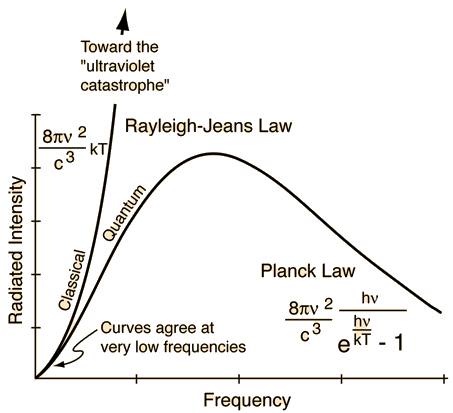
\includegraphics[width=0.9\linewidth]{pic/rj.png}
\end{minipage}
\end{center}
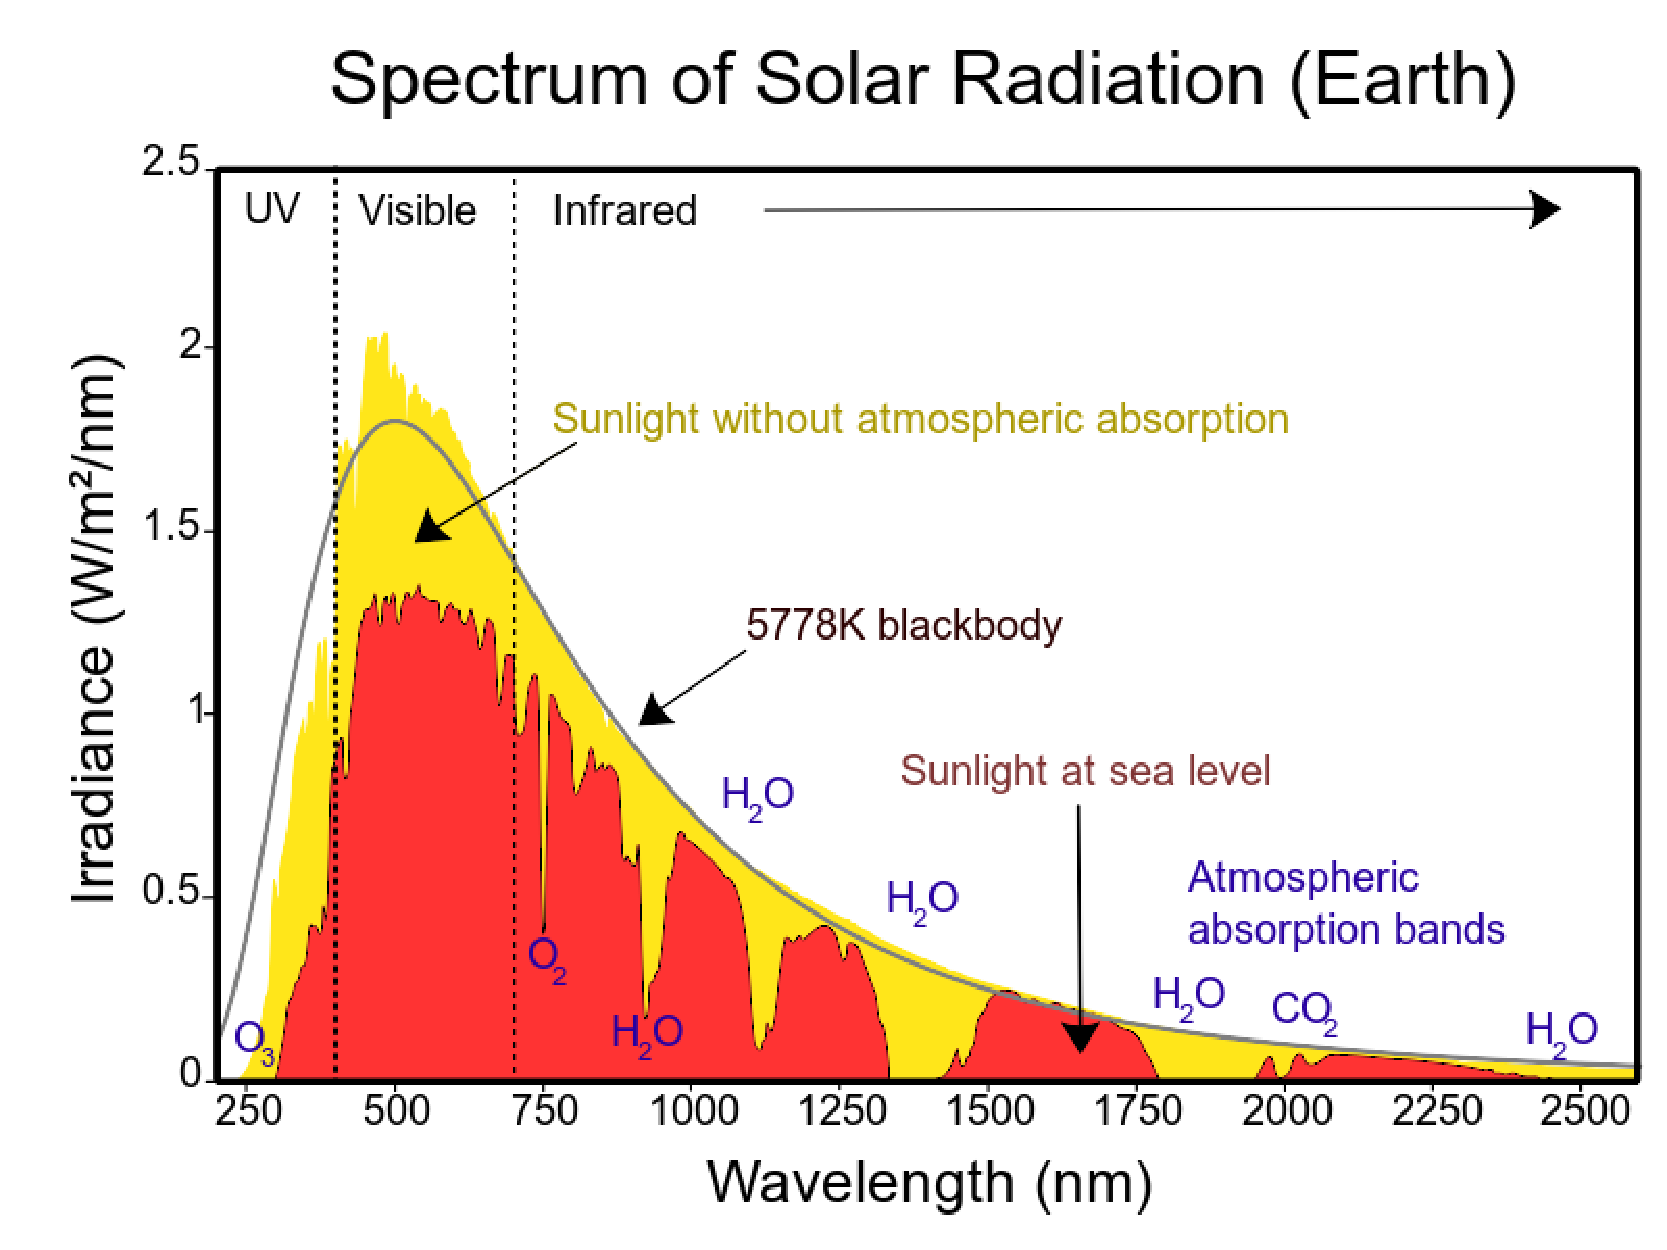
\includegraphics[width=\linewidth]{pic/p27.pdf}
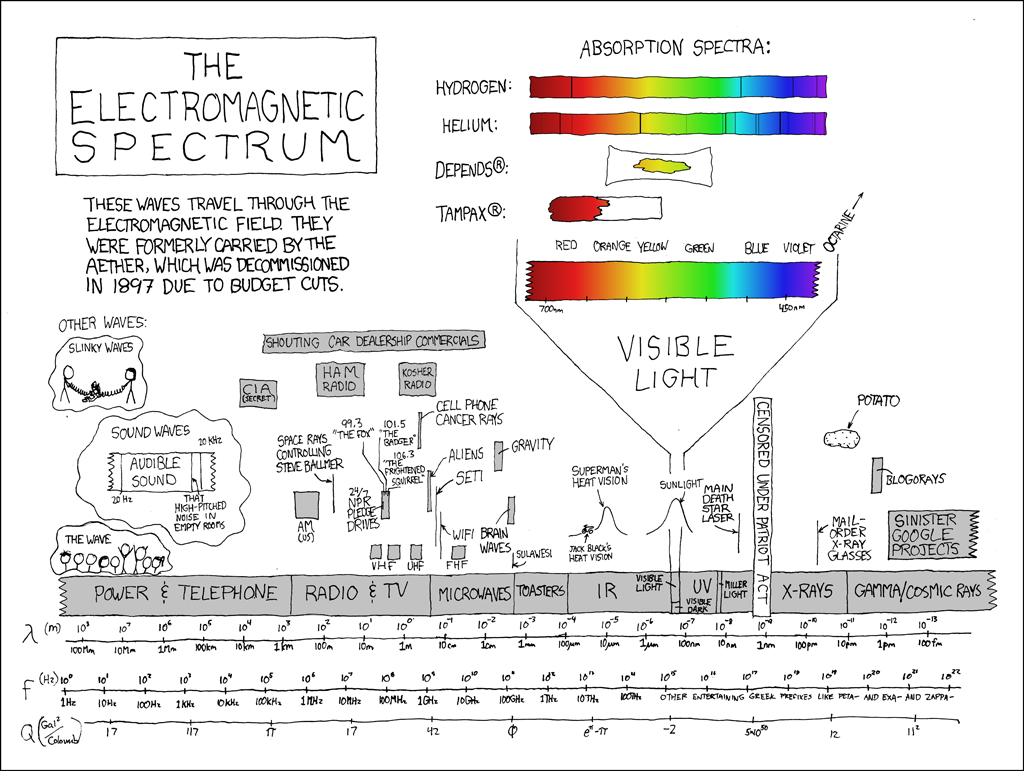
\includegraphics[height=\linewidth, angle=90]{pic/emxkcd.png}


\subsection[Strahlenoptik]{Strahlenoptik\let\thefootnote\relax\footnote{$\eps_r$: relative Permittivität im Medium, $\mu_r$: relative Permeabilität im Medium, $d$: Länge, $\alpha$: Einfalls-/Austrittswinkel, $g$: Gegenstandsweite, $b$: Bildweite, $f$: Brennweite, $r$: Krümmungsradius, $d$: Linsendicke, $M$: Mittelpunktsstrahl, $P$: Parallelstrahl, $B$: Brennstrahl}}
\begin{center}
\begin{minipage}[t]{.58\linewidth}
\vspace{0pt}
\noindent\begin{tabular}{ll}
Brechungsindex & $n = \frac{c}{v} = \sqrt{\varepsilon_r \mu_r}$\\
optische Pfadlänge & $\Delta = nd = ct$\\
Reflexionsgesetz & $\alpha_1 = \alpha_2$\\
Brechungsgesetz & $n_1 \sin \alpha_1 = n_2 \sin \alpha_2$\\
Strahlverengung & $\Delta b = \frac{\cos \alpha_2}{\cos \alpha_1}$\\
kritischer Winkel & $\sin \alpha_C = \frac{n_1}{n_2}$\\
Brewster-Winkel: & $\tan \alpha_B = \frac{n_2}{n_1}$\\
Abweichung & $\frac{n_2}{n_1} = \frac{\sin \frac{1}{2}(\alpha + \delta_m)}{\sin \frac{1}{2} \alpha}$\\
dünnes Prisma & $\frac{n_2}{n_1} = \frac{\alpha + \delta_m}{\alpha}$\\
Gauss'sche Formel & $\frac{n_1}{g} + \frac{n_2}{b} = \frac{n_2 - n_1}{r}$\\
Linsengleichung & $\frac{1}{g} + \frac{1}{b} = \frac{1}{f}$\\
Linsenschleiferformel & $\frac{1}{f} = (n-1) (\frac{1}{r_1} - \frac{1}{r_2} + \frac{(n-1)d}{n r_1 r_2})$\\
Strahlen & M $\rightarrow$ M, P $\leftrightarrow$ B\\
Vergrößerung & $V = \frac{B}{G} = -\frac{b}{g}$\\
Dioptrie & $P = 1/f[\text{m}]$\\
Vergrößerung Linse & $V_L = \frac{s_0}{f} = \frac{\sigma}{\sigma_0}$\\
Vergrößerung Mikroskop & $V_M = V_{Ob} V_{Ok} = -\frac{l}{f_{Ob}} \frac{s_0}{f_{Ok}}$\\
Vergrößerung Teleskop & $V_T = -\frac{f_{Ob}}{f_{Ok}}$\\
Spiegelgleichung & $\frac{1}{f} = -\frac{2}{r}$\\
Astigmatismus-Positionen & $\frac{1}{g} + \frac{1}{i_T} = -\frac{2}{r \cos \alpha}$\\
 & $\frac{1}{g} + \frac{1}{i_S} = -\frac{2 \cos \alpha}{r}$\\
\end{tabular}

\end{minipage}%
\begin{minipage}[t]{.4\linewidth}
\vspace{0pt}
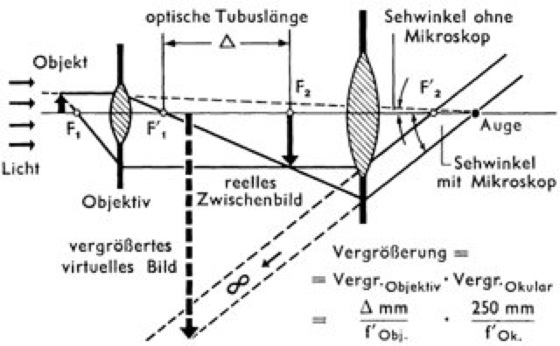
\includegraphics[width=\linewidth]{pic/mikroskop.jpg}

\end{minipage}
\end{center}

\subsection[Elektromagnetische Wellen]{Elektromagnetische Wellen\let\thefootnote\relax\footnote{}}
\begin{center}
\begin{minipage}[t]{.49\linewidth}
\vspace{0pt}
\noindent\begin{tabular}{ll}
Phase & $\omega t - k x$\\
Phasengeschw. & $v_{ph} = \frac{\omega}{k}$\\
Dopplereffekt (n.r.) & $f' = f(1+\frac{v}{c})$\\
Gruppengeschw. & $v_{gr} = \pd{\omega}{k}$\\
Wellenvektor & $\vec k = \frac{2 \pi}{\lambda} \hat e$\\
Poyntingvektor & $\vec{S} = \frac{1}{\mu_0}(\vec{E} \times \vec{B})$\\
Strahlungsdruck &  $p_S = I/c$\\
Intensität &  $I = \frac{P}{A} = |\vec{S}|$\\
Impuls &  $p = \frac{W}{c}$\\
Wellengleichung &  $\nabla^2 \vec E - \frac{1}{c^2} \ddot{\vec{E}} = \square \vec E = 0$\\
Ebene, monochr. Welle &  $\vec E = \vec E_0 \exp [\iu(\vec k \ort - \omega t + \varphi)]$\\
\end{tabular}
\end{minipage}%
\begin{minipage}[t]{.49\linewidth}
\vspace{0pt}
\begin{framed}
\begin{center}
$c = \frac{1}{\sqrt{\varepsilon_0 \mu_0}} = \frac{\omega}{k} = \lambda \cdot f$\\
$k = \frac{2\pi}{\lambda}$, $\omega = 2\pi f = \frac{2\pi}{T}$
\end{center}
\end{framed}
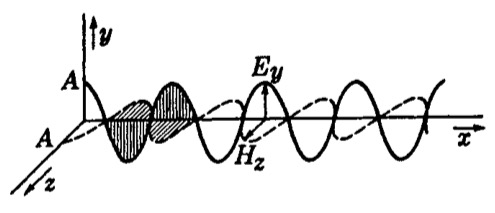
\includegraphics[width=\linewidth]{pic/emwelle.png}
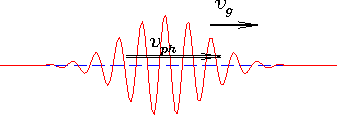
\includegraphics[width=\linewidth]{pic/vphvgr.png}
\begin{center}
\begin{framed}
$D_{n,1} = D_{n,2}$, $E_{t,1} = E_{t,2}$\\
$B_{n,1} = B_{n,2}$, $H_{t,1} = H_{t,2}$\\
Grenzflächenbedingungen
\end{framed}
\end{center}
\end{minipage}
\end{center}


\subsection[Interferenz]{Interferenz\let\thefootnote\relax\footnote{}}

\begin{center}
\begin{minipage}[t]{.6\linewidth}
\vspace{0pt}
\noindent\begin{tabular}{ll}
Young konstruktiv & $x = m \lambda \frac{D}{d}$\\
Young destruktiv & $x = (m+ \frac{1}{2}) \lambda \frac{D}{d}$\\
Fresnel'sches Biprisma & $\lambda = \frac{\Delta x d}{B + C}$\\
Intensität bei Interferenz & $I = I_1 + I_2 + 2\sqrt{I_1 I_2} \cos \theta$\\
Michelson-Interferometer &  $I = 1+\cos \theta = 1+\cos(\frac{2\pi d}{\lambda})$\\
Zeitmittel & $\langle f(t) \rangle = \lim_{T \rightarrow \infty} \frac{1}{T} \int_0^T f(t) dt$\\
\end{tabular}
\begin{framed}
Die Emission aus einer flächigen Quelle und die daraus resultierende Überlagerung an zwei Raumpunkten $P_1$ und $P_2$ kann als Beugungs- bzw. Streuproblem behandelt werden.\\
\centering\textsc{Van Cittert-Zernike-Theorem}
\end{framed}

\end{minipage}%
\begin{minipage}[t]{.4\linewidth}
\vspace{0pt}
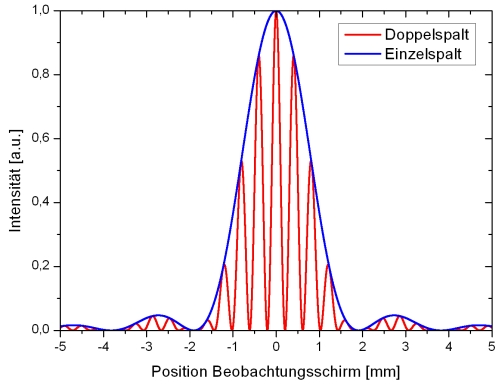
\includegraphics[width=\linewidth]{pic/interferenz.jpg}
\vspace{20px}
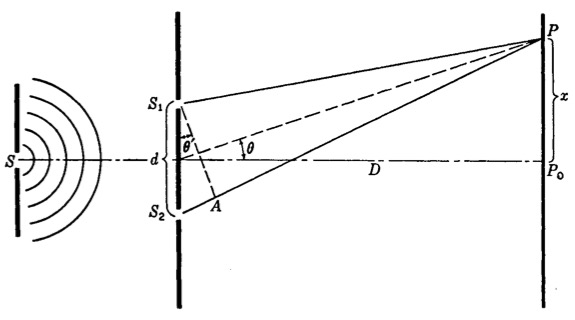
\includegraphics[width=0.9\linewidth]{pic/young.png}
\end{minipage}
\end{center}

\subsection[Beugung und Dispersion]{Beugung und Dispersion\let\thefootnote\relax\footnote{}}

\begin{center}
\begin{minipage}[t]{.6\linewidth}
\vspace{0pt}
\noindent\begin{tabular}{ll}
Beugung langer Spalt & $I = A_0^2 \frac{\sin^2 \beta}{\beta^2}$\\
& $\beta = \frac{1}{2}kb\sin \Theta$\\
& $A_0 = \frac{ab}{x}$\\
Einfall unter $i$ & $\beta = \frac{b \pi (\sin i + \sin \Theta)}{\lambda}$\\
Beugung rechteckiger Spalt & $I \sim b^2 l^2 \frac{\sin^2 \beta}{\beta^2} \frac{\sin^2 \gamma}{\gamma^2}$\\
Rayleigh-Krit. rechteckige Ap. & $\Theta = \frac{\lambda}{b}$\\
Rayleigh-Krit. runde Ap. & $\Theta = 1.22 \frac{\lambda}{D}$\\
Beugungsgitter & $d(\sin i + \sin \Theta) = m \lambda$\\
Winkeldispersion & $\frac{\Delta \Theta}{\Delta \lambda} = \frac{m}{d \cos \Theta}$\\
Auflösung Gitter & $\Delta \Theta = \frac{\lambda}{N d \cos \Theta}$\\
Resolving Power & $RP = \frac{\omega}{\delta \omega} = \frac{\nu}{\delta \nu} = \frac{\lambda}{\delta \lambda}$\\
Fresnel & $R_n = \sqrt{n \lambda L}$\\
Fresnel-Zone Fläche &  $A = \pi \lambda L$\\
Fresnellinse, fok. L. &  $l = \frac{R_1^2}{\lambda}$\\
\end{tabular}
\begin{framed}
$$d \sim \lambda/2$$
\centering Auflösungsgrenze
\end{framed}
\end{minipage}%
\begin{minipage}[t]{.4\linewidth}
\vspace{0pt}
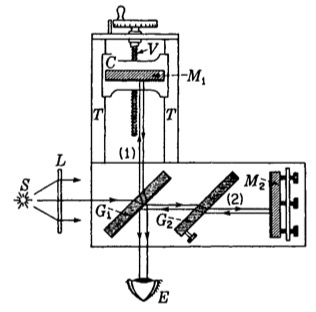
\includegraphics[width=\linewidth]{pic/michelson.png}
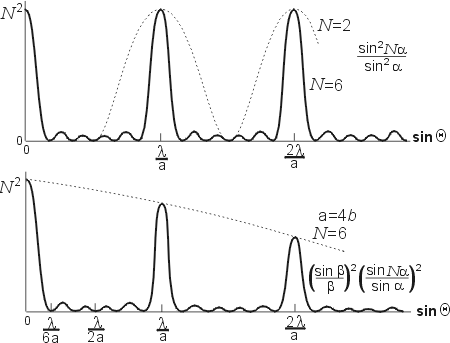
\includegraphics[width=\linewidth]{pic/gitter.png}
\end{minipage}
\end{center}


\subsection[Leiteroperatoren und kohärente Zustände]{Leiteroperatoren und kohärente Zustände\let\thefootnote\relax\footnote{}}

\begin{center}
\begin{minipage}[t]{.49\linewidth}
\vspace{0pt}
\noindent\begin{tabular}{ll}
Vernichtungsop. & $\hat a \psi_n = \sqrt n \psi_{n-1}$\\
Erzeugungsop. & $\hat a^\dagger \psi_n = \sqrt{n-1} \psi_{n-1}$\\
Vernichtungsop. & $\hat a = \frac{1}{\sqrt{2}} (\xi + \d{}{\xi})$\\
Erzeugungsop. & $\hat a^\dagger = \frac{1}{\sqrt{2}} (\xi - \d{}{\xi})$\\
Kommutator & $[a, a^\dagger] = 1$\\
Teilchenzahlop. & $\hat N = a^\dagger a = \hat N^\dagger$\\
Identität & $a a^\dagger - a^\dagger a = 1$\\
Hamiltonian hO & $\hbar \omega (a^\dagger a + 1/2)$\\
auf Teilchenzahlzustand & $\hat a \ket n = \sqrt{n} \ket{n-1}$\\
 & $\hat a^\dagger \ket n = \sqrt{n+1} \ket{n+1}$\\
Vakuumzustand & $\hat a \ket 0 = 0$\\
Quantisierung EM-Feld & $\vec A_k = \sqrt{\frac{\hbar}{2 \varepsilon_0 V \omega_k}} \hat a_k \vec e_k$\\
 & $\vec A_k^* = \sqrt{\frac{\hbar}{2 \varepsilon_0 V \omega_k}} \hat a_k^\dagger \vec e_k$\\
\end{tabular}
\end{minipage}%
\begin{minipage}[t]{.49\linewidth}
\vspace{0pt}
\begin{tabular}{ll}

\end{tabular}
\end{minipage}
\end{center}


\subsection[Kohärenz]{Kohärenz\let\thefootnote\relax\footnote{}}

\begin{center}
\begin{minipage}[t]{.55\linewidth}
\vspace{0pt}
\noindent\begin{tabular}{ll}
Gesamtintensität & $I = I_1 + I_2 + 2 \sqrt{I_1 I_2} \Re[k_1 k_2 \gamma^1 (x_1, x_2)]$\\
Korrelationsfunktion & $\Gamma_{12}(\tau) = \Re \{ \frac{1}{T} \int_0^T \vec E_1(t) \cdot \vec E_2^*(t + \tau) dt$\\
Lorentzpuls & $\gamma^{(1)} = \exp{-i \omega_0 \tau} \exp{-\abs{\tau} / \tau_c}$\\
Gaußpuls & $\gamma^{(1)} = \exp{-i \omega_0 \tau} \exp{-\frac{\pi}{2} (\frac{\tau}{\tau_c})^2}$, $\tau_c = \frac{\sqrt{8 \pi \ln 2}}{\Delta \omega}$\\
Kohärenzlänge & $l_c = c \langle \tau_0 \rangle = \frac{c}{\Delta \nu}$\\
Frequenzbandbreite &  $\Delta \omega = \frac{2\pi}{\tau_0}$\\
Linienbreite &  $\Delta \lambda = \frac{\lambda_0^2}{l_c}$\\
Kohärenzlänge & $l_t = \frac{\lambda r}{s} = \frac{\lambda}{\theta_s}$ mit $\theta_s$ Winkelauflösung\\
$l_t$ runde Quelle: & $l_t = \frac{1,22 \lambda}{\theta_s}$\\
Kontrast &  $V = \frac{I_{max} - I_{min}}{I_{max} + I_{min}} = \frac{2\sqrt{I_1 I_2} \cdot \abs{\gamma^1}}{I_1 + I_2}$\\
Kontrast (gleiche Amp.) & $V = \abs{\gamma_{12}}$\\
Kohärenz 2. Ordnung & $\gamma^{2}(\tau) = \frac{\erw{I(t) I(t+\tau)}}{\erw{I(t)}^2}$\\
\end{tabular}
\end{minipage}%
\begin{minipage}[t]{.44\linewidth}
\vspace{0pt}
\begin{tabular}{ll}

\end{tabular}
\end{minipage}
\end{center}

\subsection[Optische Elemente]{Optische Elemente\let\thefootnote\relax\footnote{}}

\begin{minipage}[t]{.49\linewidth}
\vspace{0pt}
\noindent\begin{tabular}{ll}
Phasenplatte & $H = \hbar (\omega + \phi) \hat a^\dagger \hat a$\\
effektive Phasenverschiebung & $\phi t = \varphi$\\
Strahlteiler & $H = \hbar \chi (\hat a^\dagger \hat b + \hat b^\dagger \hat a)$\\
Parametrische Fluoreszenz & $H_i = \hbar G (\hat a_1^\dagger \hat a_2^\dagger \exp{i \varphi} + \hat a_1 \hat a_2 \exp{-i \varphi})$\\
Parameter & $r = Gt = \frac{G l}{v}$\\
squeezed state & $\sigma_Q^2 \sigma_P^2 \geq 1$ mit $\sigma_Q^2 \neq \sigma_P^2$\\
\end{tabular}
\end{minipage}%
\begin{minipage}[t]{.49\linewidth}
\vspace{0pt}

\end{minipage}

\subsection{Absorption}

\begin{center}
\begin{minipage}[t]{.5\linewidth}
\vspace{0pt}
\noindent\begin{tabular}{ll}
Lambert-Beer'sches Gesetz & $I(x) = I_0 e^{-\alpha x}$\\
Absorptionskoeff. & $\alpha(\omega) = \frac{2\omega}{c}k(\omega)$\\
Plasmafrequenz & $\omega_p^2 = \frac{4\pi n e^2}{m}$\\
Produktion freier Ladungen & $\pd{n}{t} = D \pdd{n}{z} + G - R$\\
Erzeugungsrate & $G = \frac{\alpha (1-R)}{\hbar \omega \tau_p} Q \exp[-\int_0^z \alpha dz']$\\
free carrier thermalization rate & $\frac{1}{\tau_{e,e}} = K \frac{(\pi k_B T)^2 + \epsilon^2}{1 + \exp(-\epsilon / (k_B T))}$\\
Auger-Relaxionsrate & $R_C = C n^3$\\
Heizen mit CW-Laser & $\rho C_p \pd{T}{t} = \nabla (\kappa \nabla T) + \pd{Q}{t}$\\
Temperaturverteilung & $T(r) \sim \exp[-r^2 / l_{tot}^2]$\\
Ausdehnung Temperaturspot & $l_{tot} = l_{em} + l_{T}$\\
Ausdehnung Heizspot & $l_{em} \sim \lambda / \Im(n)$\\
Ausdehnung Wärmeleitung & $l_{T} \sim \sqrt{\tau_p D}$\\

Heizen mit fs-Laser & \makecell[l]{$C_e \pd{T_e}{t} = \nabla [\kappa_e \nabla T_e] - \Gamma_{e-ph}[T_e - T] + Q$ \\ $C \pd{T}{t} = \nabla [\kappa \nabla T] - \Gamma_{e-ph} [T_e - T]$}\\


\end{tabular}
\end{minipage}%
\begin{minipage}[t]{.5\linewidth}
\vspace{0pt}
\begin{tabular}{ll}

\end{tabular}
\end{minipage}
\end{center}



\subsection[Nichtlineare Optik]{Nichtlineare Optik\let\thefootnote\relax\footnote{}}

%\begin{center}
\begin{minipage}[t]{.49\linewidth}
\vspace{0pt}
\noindent\begin{tabular}{ll}
Polarisation (Antwort) & $P = \varepsilon_0 \chi^1 E + \varepsilon_0 \chi^2 E^2 + \varepsilon_0 \chi^3 E^3 + ...$\\
Phasengleichheit & $\vec k = \vec k_1 + \vec k_2$\\
Wellengleichung & $\nabla \times (\nabla \times E) = \frac{1}{c^2} \pdd{E}{t} + \frac{4\pi}{c^2} \pdd{P_l}{t} + \frac{4\pi}{c^2} \pdd{P_{nl}}{t}$\\
Verschiebungsdichte & $\vec D = \vec E + 4 \pi \vec P$\\
Kerr-Effekt & $n = n_0 + n_2 I$\\
Intensität im n.l. Medium & $I_2(l) \sim \gamma_2^2 I_0^2 l^2 (\frac{\sin(\Delta k l/2)}{\Delta k l / 2})^2$\\
\end{tabular}
\end{minipage}%
\begin{minipage}[t]{.49\linewidth}
\vspace{0pt}

\end{minipage}
%\end{center}



\subsection[Laserphysik]{Laserphysik\let\thefootnote\relax\footnote{}}

\begin{minipage}[t]{.49\linewidth}
\vspace{0pt}
\noindent\begin{tabular}{ll}
räumliche Kohärenz zufällige Quelle & $r_c = \frac{\lambda z}{a}$\\
räumliche Kohärenz Laser & $r_c \sim a$\\
Divergenz pertiell kohärenter Strahlen & $\Theta = \lambda / \sqrt{S}$\\
Divergenz kohärenter Strahl & $\Theta = \lambda / D$\\
Mittlere Leistung & $\hat P = E \cdot RR$\\
Peakleistung & $P_{peak} = E/\tau$\\
Fluence & $F = E/s = 4E/\pi D^2$\\
Intensität & $I = F/\tau = E/D^2 \tau$\\

\end{tabular}
\end{minipage}%
\begin{minipage}[t]{.49\linewidth}
\vspace{0pt}

\end{minipage}



\subsection[Emission und Photolumineszenz]{Emission und Photolumineszenz\let\thefootnote\relax\footnote{}}

\begin{minipage}[t]{.49\linewidth}
\vspace{0pt}
\noindent\begin{tabular}{ll}

\end{tabular}
\end{minipage}%
\begin{minipage}[t]{.49\linewidth}
\vspace{0pt}

\end{minipage}



\subsection[2-Niveau-System]{2-Niveau-System\let\thefootnote\relax\footnote{}}

\begin{minipage}[t]{.49\linewidth}
\vspace{0pt}
\noindent\begin{tabular}{ll}


\end{tabular}
\end{minipage}%
\begin{minipage}[t]{.49\linewidth}
\vspace{0pt}

\end{minipage}



\newpage
\section{Quantenmechanik}

\subsection{Wellenfunktion}

\begin{minipage}[t]{.45\linewidth}
\vspace{0pt}
\noindent\begin{tabular}{ll}

Schrödingergl. & $i \hbar \pd{}{t} \psi = - \frac{\hbar^2}{2m}\pdd{}{x} \psi + V \psi$\\
de Broglie-Relation & $p = \bar k$\\
Wahrscheinlichkeitsdichte & $\abs{\psi}^2 dx$\\
Normierung & $\int_{-\infty}^{\infty} \abs{\psi}^2 dx = 1$\\
Impuls & $p = \frac{\hbar}{i}\pd{}{x}$\\
Ortserwartungswert & $\erw x = \int_{-\infty}^{\infty} \psi^* x \psi dx$\\
Geschwindigkeiterw. & $\erw v = \int_{-\infty}^{\infty} \psi^* (\frac{\hbar}{i m}\pd{}{x}) \psi dx$\\
Unschärferelation & $\sigma_x \sigma_{p_x} \geq \hbar/2$\\

\end{tabular}
\end{minipage}%
\hspace{0.02\linewidth}
\begin{minipage}[t]{.45\linewidth}
\vspace{0pt}
\begin{tabular}{ll}
\toprule


\end{tabular}
\end{minipage}


\subsection{Zeitabhängige Schrödingergleichung}

\begin{minipage}[t]{.5\linewidth}
\vspace{0pt}
\noindent\begin{tabular}{ll}

Zeitunabg. SG & $i \hbar \pd{}{t} \psi = (-\frac{\hbar^2}{2m}\dd{}{x} + V(x))\psi$\\
Separationsansatz & $\psi(x, t) = \phi(x) f(t)$\\
Lösung für $E$ & \makecell[l]{$i \hbar \d{}{t} f(t) = E f(t)$\\$(-\frac{\hbar^2}{2m} \dd{}{x} + V) \phi(x) = E \phi (x)$}\\
Lösung & $\psi(x, t) = \phi(x) \exp(- \frac{i}{\hbar} E t)$\\
angeregte Zustände & $n = 1, 2, ...$ Knoten\\
Stetigkeit & \makecell[l]{$\phi$ stetig\\$\d{\varphi}{x}$ stetig, wenn $V$ endlich}\\

\textbf{Asym. unendliches Kastenpotential} & \\
Energien & $E_n = \frac{\hbar^2 \pi^2}{2ma^2} n^2$\\
Wellenfunktionen & $\phi_n(x) = \sqrt{\frac{2}{a}} \sin (\frac{n \pi}{a}x)$\\

\textbf{Freies Teilchen} & \\
Potential & $V(x) = 0$\\
Wellenfunktion & $\psi (x, t) = \frac{1}{\sqrt{2\pi}} \int_{-\infty}^{+\infty} dk \phi(k) \exp(i[kx - \hbar k^2 t / 2m])$\\

\textbf{Delta-Potential} & \\
Potential & $V(x) = - \alpha \delta (x)$\\
Bedingung & $E < 0, \alpha > 0$\\
Wellenfunktion & $\frac{\sqrt{m\alpha}}{\hbar} \exp(-\frac{m\alpha}{\hbar^2} \abs{x})$\\
Energien & $E = - \frac{m\alpha^2}{2\hbar^2}$\\
Reflexionskoeff. & $R = 1/(1 + \frac{2\hbar^2 E}{m\alpha^2})$\\
Transmissionskoeff. & $T = 1/(1 + \frac{m\alpha^2}{2\hbar^2 E})$\\


\end{tabular}
\end{minipage}%
\begin{minipage}[t]{.5\linewidth}
\vspace{0pt}
\begin{tabular}{ll}


\end{tabular}
\end{minipage}


\begin{minipage}[t]{.5\linewidth}
\vspace{0pt}
\noindent\begin{tabular}{ll}

\textbf{Harmonischer Oszillator} & \\
Potential & $V(x) = \frac{m\omega^2}{2}x^2$\\
Energien & $E_n = (n + 1/2) \hbar \omega$\\
Wellenfunktionen & $\phi_n(x) = A_n (a^+)^n \exp(-\frac{m\omega}{2\hbar}x^2)$\\
Leiteroperatoren & \makecell[l]{$a_+ = \frac{1}{\sqrt{2m}} (\frac{\hbar}{i} \d{}{x} + i m \omega x)$ \\ $a_- = \frac{1}{\sqrt{2m}} (\frac{\hbar}{i} \d{}{x} - i m \omega x)$}\\
Hamiltonian & $H = a_- a_+ - \hbar \omega /2$\\
Impuls & $p = \sqrt{\frac{m}{2}} (a_+ + a_-)$\\
Ort & $x = i \sqrt{\frac{1}{2m\omega^2}} (a_- - a_+)$\\
Kanonische Kommutatorrel. & $[x, p] = i\hbar$\\
Kommutator $a_-, a_+$ & $[a_-, a_+] = \hbar \omega$\\
Virialsatz & $\frac{1}{2}\erw{E} = \erw{T} = \erw{V}$\\


\end{tabular}
\end{minipage}%
\begin{minipage}[t]{.5\linewidth}
\vspace{0pt}
\begin{tabular}{ll}

\end{tabular}
\end{minipage}





\subsection{Hilbertraum}

\begin{minipage}[t]{.55\linewidth}
\vspace{0pt}
\noindent\begin{tabular}{ll}

Vektoren & $\ket{\alpha}$ im $\mathsc{C}$-Vektorraum\\
Skalarprodukt & $\braket{\alpha}{\beta} = \int \alpha^* (x) \beta(x) dx$\\
hermitscher Operator & $\braket{\alpha}{A \beta} = \braket{A \alpha}{\beta}$\\
quadratintegrabel & $\int_{-\infty}^{+\infty} \psi^*(x) \psi(x) dx < \infty$\\
Messgröße & $\erw{A} = \bra{\psi} A \ket{psi}$\\
Varianz & $\sigma^2 = \erw{A^2} - \erw{A}^2$\\
Einheitsoperator & $\mathcal{1} = \sum_n \ket{e_n}\bra{e_n}$\\
Projektionsoperator & $P = P^2$\\
Wahrscheinlichkeit & $\abs{c_n} = \abs{\braket{e_n}{\psi}}^2$\\
Heisenberg'sche Unschärfe & $\sigma_A^2 \sigma_B^2 \geq (\frac{1}{2i} \erw{[A, B]})^2$\\
totale Zeitableitung & $\d{}{t} \erw{A} = \frac{i}{\hbar} \erw{[H, A]} + \erw{\pd{A}{t}}$\\




\end{tabular}
\end{minipage}%
\begin{minipage}[t]{.45\linewidth}
\vspace{0pt}

\begin{framed}
$[A, B] = AB - BA$\\
$[A, B] + [B, A] = 0$\\
$[A, A] = 0$\\
$[A, B+C] = [A, C] + [B, C]$\\
$[A, BC] = [A, B]C + B[A, C]$\\
$[AB, C] = [A, C]B + A[B, C]$\\
$[A, [B, C]] + [C, [A, B]] + [B, [C, A]] = 0$\\
$[A, B^n] = n B^{n-1}[A, B]$\\
$[A^n, B] = n A^{n-1}[A, B]$\\
$e^A B e^{-A} = B + [A, B] + \frac{1}{2!}[A, [A,B]] + \frac{1}{3!}[A, [A, [A, B]]]$\\
$\{A, B\} = AB + BA$
\end{framed}

\begin{tabular}{ll}


\end{tabular}
\end{minipage}





\begin{center}
\begin{minipage}[t]{.45\linewidth}
\vspace{0pt}
\noindent\begin{tabular}{ll}
\toprule



\bottomrule
\end{tabular}
\end{minipage}%
\hspace{0.02\linewidth}
\begin{minipage}[t]{.45\linewidth}
\vspace{0pt}
\begin{tabular}{ll}
\toprule


\end{tabular}
\end{minipage}
\end{center}














\subsection{Thermodynamik und QM}

\begin{center}
\begin{minipage}[t]{.35\linewidth}
\vspace{0pt}
\noindent\begin{tabular}{ll}
\toprule

Energiequantisierung &  $E_n = nh\nu$\\
Bohr &  $\frac{Ze^2}{4\pi \varepsilon_0 r_n^2} = m \omega^2 r_n$\\
Drehimpuls &  $p_{\varphi_n} = n \hbar = L_n$\\
Wellenfunktion & $\psi(\ort, t) = \psi_0 \cdot \exp[\iu (\vec k \cdot \ort - \omega t)]$\\

\bottomrule
\end{tabular}
\end{minipage}%
\begin{minipage}[t]{.65\linewidth}
\vspace{0pt}
\begin{tabular}{ll}
\toprule


\end{tabular}
\end{minipage}
\end{center}



\begin{center}
\begin{minipage}[t]{.35\linewidth}
\vspace{0pt}
\noindent\begin{tabular}{ll}
\toprule
Photoeffekt Grenzwellenlänge & $\lambda_G = \frac{hc}{W_A}$\\
Duane+Hund &  $U \cdot \lambda_{min} = \frac{hc}{e} = 1240$Vnm\\
charakt. Spektrum &  $\Delta E = h\nu$\\
Bremsstrahlung en.reichstes Quant &  $E = Ue = \frac{hc}{\lambda_min}$\\
\bottomrule
\end{tabular}
\end{minipage}%
\begin{minipage}[t]{.65\linewidth}
\vspace{0pt}
\begin{tabular}{ll}
\toprule


\end{tabular}
\end{minipage}
\end{center}




\begin{center}
\begin{minipage}[t]{.35\linewidth}
\vspace{0pt}
\noindent\begin{tabular}{ll}
\toprule
Comptonstreuung & $\lambda_f = \frac{h}{m_0 c} (1- \cos \theta) + \lambda_i$
Rückstreuung & $\lambda_c = \frac{h}{m_0 c} = 2,43$pm\\
Exp. Abfall &  $N(t) = N_0 \cdot \exp (- \lambda t)$ mit $\lambda = \ln 2 / T_{1/2}$\\
\bottomrule
\end{tabular}
\end{minipage}%
\begin{minipage}[t]{.65\linewidth}
\vspace{0pt}
\begin{tabular}{ll}
\toprule


\end{tabular}
\end{minipage}
\end{center}


\subsection{Heisenberg}

\begin{framed}
$$\Delta x \cdot \Delta p_x \geq \hbar/2$$
\end{framed}

\begin{center}
\begin{minipage}[t]{.35\linewidth}
\vspace{0pt}
\noindent\begin{tabular}{ll}
\toprule
Aufenthaltswahrsch. in $\Delta x$ & $P_{\Delta x} = \int_{x_0}^{x_1} \psi^2(x) dx$\\
$\Delta k \cdot \Delta x = 2\pi$\\
\bottomrule
\end{tabular}
\end{minipage}%
\begin{minipage}[t]{.65\linewidth}
\vspace{0pt}
\begin{tabular}{ll}
\toprule

\end{tabular}
\end{minipage}
\end{center}


\subsection{Schrödinger}

\begin{center}
\begin{minipage}[t]{.35\linewidth}
\vspace{0pt}
\noindent\begin{tabular}{ll}
\toprule

unendlicher Potentialtopf von 0 bis a & $\psi_n(x) = \sqrt{\frac{2}{a}} \sin (\frac{n \pi}{a}x)$\\
$n$-te Energie &  $E_n = n^2 \frac{h^2}{8ma^2}$\\
unendl. Pot.topf von -a bis a &  $\psi_n(x) = \sqrt{\frac{1}{2a}} \cos (\frac{(n+1/2) \pi}{a}x)$\\
Erw.wert &  $\langle x \rangle = \int_0^a x \cdot \abs{\psi(x,t)}^2 dx$\\
Randbedingungen &  $\psi, \psi'$ bei $x=0, x=a$ stetig\\
Normierung &  $1 = \int_0^a \abs{\psi}^2 dx$\\
Transmissionskoeff. &  $E>V_0$: $T = \frac{4E(E-V_0)}{4E(E-V_0)+V_0^2 \cdot \sin^2 (k_2 a)}$\\
$E<V_0$: & $T = \frac{4E(E-V_0)}{4E(E-V_0)+V_0^2 \cdot \sinh^2 (k_2 a)}$\\
Transmission &  $\lambda_E = \frac{h}{\sqrt{2m(E-V_0)}}$\\
dunnow & $k_2 = \frac{\sqrt{2m(E-V_0)}}{\hbar}$\\
Reflektion & $R = \frac{(k_1-k_2)^2}{(k_1 + k_2)^2}$\\
harm. Osz. & $E_0 = \frac{1}{2} \hbar \omega_0$\\
\bottomrule
\end{tabular}
\end{minipage}%
\begin{minipage}[t]{.65\linewidth}
\vspace{0pt}
\begin{tabular}{ll}
\toprule


\end{tabular}
\end{minipage}
\end{center}


\begin{framed}
\begin{align*}
\iu \hbar \pd{}{t} \psi =& - \frac{\hbar^2}{2m} \Delta \psi + V  \psi\\
\hat H \psi =& E \psi
\end{align*}
\end{framed}


\subsection{Tunneleffekt}


\subsection{Quantenmechanischer Oszillator}


\subsection{Grundlagen}
\begin{framed}
$(-\frac{\hbar^2}{2m} \nabla^2 + V)\psi = \iu \hbar \pd{}{t} \psi$
\end{framed}
\begin{center}
\begin{minipage}[t]{.35\linewidth}
\vspace{0pt}
\noindent\begin{tabular}{ll}
\toprule
totaler W.querschnitt &  $\sigma = \frac{pA}{N_{\text{target}}}$\\
diff. W.querschnitt &  $(\d{\sigma}{\Omega})_{\vartheta} = (\d{p}{\Omega})_{\vartheta} (\frac{A}{N_{\text{target}}})$\\
für Zählraten &  $\Delta p = \frac{f_{\Omega}}{f_0}$\\
axialsymmetrisch &  $(\d{\sigma}{\Omega})_{\vartheta} = \frac{b}{\sin\vartheta} \abs{\d{b}{\vartheta}}$\\
Stoßparameter & $b = \frac{Z_1 Z_2 e^2}{8\pi \varepsilon_0 E_{kin}} \cot \frac{\vartheta}{2}$\\
kA & $f_{\Omega} = \mu f_0 \d{\sigma}{\Omega} \Delta \Omega$\\
Rutherford-Streuung &  $(\d{\sigma}{\Omega})_{\vartheta} \sim \frac{1}{\sin^4 (\frac{\vartheta}{2})}$\\
Probleme Rutherford-Modell & 1. beschl. Ladungen, Energieverlust; 2. Existenz atomarer Spektrallinien\\
H-Spektrum &  $\frac{1}{\lambda} = R_{\infty} (\frac{1}{n_a^2} - \frac{1}{n_b^2})$ mit $R_{\infty} = \frac{m_e e^4}{8 \varepsilon_0^2 h^3 c} = 109677 \text{cm}^{-1}$\\
Serien & Lyman ($n_a = 1$, UV), Balmer (2, V), Paschen (3, IR), Brackett (4), Pfund (5), Humphreys (6)\\
Rydberg-Konstante & $R = \frac{R_{\infty}}{1+\frac{m_e}{M}}$\\
Bohr'sche Quantenbedingung & $l = n \hbar$\\
Radius &  $r_n = \frac{h^2 \varepsilon_0}{\pi \mu e^2} \frac{n^2}{Z}$

Feinstrukturkonst. &  $\alpha = \frac{e^2}{4\pi \varepsilon_0 \hbar c} \approx \frac{1}{137}$\\
reduz. Masse &  $\mu = \frac{m_1 m_2}{m_1 + m_2}$\\
Energieeigenwerte &  $E_n = \frac{\mu e^4}{8 \varepsilon_0^2 \hbar^2} \frac{1}{n^2} = \frac{E_0}{n^2}$\\
relat. & $E = \sqrt{m_0^2c^4 + p^2c^2}$\\
Coulomb-Pot. &  $V = - \frac{Ze^2}{4\pi \varepsilon_0 r}$\\
kA & $\omega_n = \frac{v_n}{r_n} = \frac{e^4 m}{16 \pi^2 \varepsilon_0^2 \hbar^2 n^3}$\\
\bottomrule
\end{tabular}
\end{minipage}%
\begin{minipage}[t]{.65\linewidth}
\vspace{0pt}
\begin{tabular}{ll}
\toprule

\end{tabular}
\end{minipage}
\end{center}



Bohr'sche Postulate:
\begin{enumerate}
\item $\exists$ diskrete Bahnen mit $E_n$, auf denen sich $e^-$ strahlungsfrei bewegen können
\item Strahlungsemission/-absorption findet an Übergängen statt mit $hf = \Delta E$ und $E_n = R_{\infty} \frac{hc}{n^2}$
\item Korrespondenzprinzip
\end{enumerate}

Extraktion von E und p \dotfill  $E \psi = -i\hbar \pd{}{t} \psi$, $\vec p \psi = - i \hbar \nabla \psi$\\
$E_{ges} = \frac{p^2}{2m} + eV(\ort) \rightarrow - \frac{\hbar^2}{2m}
\nabla^2 + eV(\hat r) = \hat H$\\
$\hat L = \hat r \times \hat p$\\
$[\hat H, \hat L_i] = 0, [\hat H, \hat L^2] = 0, [\hat L_i, \hat L_j] = i\hbar \hat L_k$\\
$\hat L^2 \ket{Y_{l,m} (\theta, \varphi)} = l(l+1)\hbar^2 \ket{Y_{l,m} (\theta, \varphi)}$\\
$\hat L_z \ket{Y_{l,m} (\theta, \varphi)} = m\hbar \ket{Y_{l,m} (\theta, \varphi)}$\\
$\nabla^2 = \pdd{}{r} + \frac{2}{r}\pd{}{r} + \frac{\hat L^2}{r^2 \hbar^2}$\\
$\hat H = \sum \hat H_i (x_i) \Rightarrow \psi(\ort) = \Pi \psi_i (x_i)$\\
$E = \frac{\hbar^2}{2m} (q_1^2 + q_2^2 + q_3^2)$\\
$Y_{l,m} (\theta, \varphi) = e^{im\varphi} \cdot P_l^m (\cos \theta)$\\

HERE GOES QT2\\






\section{Atom- und Molekülphysik}
\subsection{Grobstruktur}

\begin{center}
\begin{minipage}[t]{.35\linewidth}
\vspace{0pt}
\noindent\begin{tabular}{ll}
\toprule
Potential & $V(r) = -\frac{Ze^2}{4\pi \varepsilon_0 r}$\\
SG & $\{-\frac{\hbar^2}{2m} [\frac{1}{r^2} \pd{}{r} (r^2 \pd{}{r}) - \frac{\hat L^2}{\hbar^2 r^2}] + V(r) \} \psi(\ort) = E \psi(\ort)$\\
Ansatz: & $\psi_{E, l, m} = R_{E, l}(r) \cdot Y_{l,m} (\theta, \varphi)$\\
weiter mit & $R_{E, l}(r) = \frac{u_{E, l}(r)}{r}$\\
dann & $\Rightarrow \{-\frac{\hbar^2}{2m} \d{}{r} + \frac{l(l+1)\hbar^2}{2mr^2} + V(r)\} u_{E, l}(r) = E u_{E, l}(r)$\\
Energie & $W(r) dr = 4\pi r^2 |\psi (r, \vartheta, \varphi) |^2 dr$\\
für H in 1s & $W = \frac{4}{a_0^3} \int_b^c r^2 \exp(\frac{-2r}{a_0})dr = \\ \frac{4}{a_0^3} [\exp(\frac{-2r}{a_0})(\frac{-a_0 r^2}{2} - \frac{a_0^2 r}{2} - \frac{a_0^3}{4})]$\\
Max bei & $r_m = \frac{a_0}{Z}$\\
Erwartungswert Ort & $\langle r \rangle = \frac{4}{a_0^3}\int_0^{\infty} r^3 \exp (\frac{-2r}{a_0}) dr = \frac{4}{a_0^3}[\exp(\frac{-2r}{a_0})(\frac{-a_0 r^3}{2} - \frac{3a_0^2 r^2}{4} - \frac{a_0^3 r}{4} - \frac{3a_0^4}{8})]$\\
\bottomrule
\end{tabular}
\end{minipage}%
\begin{minipage}[t]{.65\linewidth}
\vspace{0pt}
\begin{tabular}{ll}
\toprule


\end{tabular}
\end{minipage}
\end{center}



\subsection{Feinstruktur}

\begin{center}
\begin{minipage}[t]{.35\linewidth}
\vspace{0pt}
\noindent\begin{tabular}{ll}
\toprule
Bahndrehimpuls &  $\vec l = \ort \times \vec p = m_e \ort \times \vec v$\\
mag. Moment &  $\vec \mu = I \vec A = - \frac{1}{2} e \ort \times \vec v$\\
damit &  $\vec \mu = - \frac{e}{2m} \vec l$\\
in homog. $B$-Feld &  $E = - \vec \mu \cdot \vec B$, $\vec M = \vec \mu \times \vec B$\\
normaler Zeeman-Effekt &  Aufspaltung in $(2l+1)$ äquidistante Energieniveaus: $\Delta E = \mu_B B$\\
Kreiselgleichung & $\d{\vec \mu}{t} = - \frac{e}{2m} \vec \mu \times \vec B$ Kreiselgleichung mit Präzessionsfreq. $\vec \omega_L = - \frac{e \vec B}{2m}$ (Larmor-Frequenz)\\
mag. Dipol & $\vec \mu_l = - \frac{e \hbar}{2m_e} \frac{\vec l}{\hbar} = \mu_B \frac{\vec l}{\hbar}$\\
Kernmagneton & $\mu_K = \frac{e \hbar}{2m_p} << \mu_B$\\
allg. Drehimpuls &  $\vec \mu_{l,s} = g_{l,s} \mu_B \frac{(\vec l, \vec s)}{\hbar}$\\
Stern-Gerlach: & neutrale Ag-Atome durch inhomog. $B$-Feld\\
Kraft im Stern-Gerlach & $F_z = \mu_z \pd{B_z}{z} \rightarrow$ zwei Werte\\
innerer Drehimpuls &  $s = \frac{1}{2} \hbar$\\
mag. Spinmoment &  $\vec \mu_s = g_s \mu_B \frac{\vec s}{\hbar}$\\
Kommutator Spin & $[\hat S_i, \hat S_j] = i\hbar \hat S_k, [\hat S^2, \hat S_z] = 0$\\
Gesamtdrehimpuls &  $j = \abs{\vec l + \vec s} = j(j+1)$\\
Magnetfeld Bahndrehimpuls &  $\vec B = \frac{\mu_0 Z e}{8\pi m_e r^3} \vec l$\\
WW-Energie Spin-Bahn-Kopplung &  $\Delta E_{ls} = g_s \mu_B \frac{\mu_0 Z e}{8 \pi \hbar m_e r^3} (\vec s \cdot \vec l)$\\
kA & $\vec s \cdot \vec l = \frac{1}{2} (\vec \jmath^2 - \vec l^2 - \vec s^2)$\\
Energie Spin-Bahn-Kopplung & $E_{nlj} = E_n + \frac{a}{2} (j(j+1) - l(l+1) - s(s+1))$ mit $a = \frac{\mu_0 Z e^2 \hbar^2}{8\pi m_e^2 r^3}$\\
Energieaufspaltung Spin-Bahn-Kopplung & $\Delta E_{ls} = -E_n \frac{Z^2 \alpha^2}{n l (l+1)}$\\
anormaler Zeeman-Effekt ($2j+1$, nicht äquidistant) & $\Delta E_{m_j, {m_j - 1}} = g_j \mu_B B$\\
Gyromagnetisches Verhältnis & $g_j = 1+ \frac{j(j+1) + s(s+1) - l(l+1)}{2j(j+1)}$\\
kA & $\Delta m_j = \pm 1$: zirkular\\
kA & $\Delta m = 0$: linear zu B\\
Bezeichnung &  $n ^{2s+1}X_j$\\
Spin-Bahn-Kopplungskonstante & $a = \frac{\mu_0 Z e^2 \hbar^2}{8\pi m_e^2 r^3}$\\
kA & $\Delta E = \frac{Z e^2 \mu_0}{8 \pi m_e^2 r^3}$\\
kA & $B = \frac{ma}{\hbar^2 e} \sqrt{l(l+1)}\hbar$\\
kA & $\vec j^2 = \vec l^2 + \vec s^2 + 2 \vec l \vec s$\\
\bottomrule
\end{tabular}
\end{minipage}%
\begin{minipage}[t]{.65\linewidth}
\vspace{0pt}
\begin{tabular}{ll}
\toprule


\end{tabular}
\end{minipage}
\end{center}




\subsection{Hyperfeinstruktur}

\begin{center}
\begin{minipage}[t]{.35\linewidth}
\vspace{0pt}
\noindent\begin{tabular}{ll}
\toprule
Kernspin & $|I| = \sqrt{I(I+1)}\hbar$\\
mag. Dipol & $\mu_I = g_I \mu_K \frac{I}{\hbar}$\\
Gesamtdrehimpuls & $\vec F = \vec j + \vec I$\\
Energieverschiebung & $\Delta E_{HFS} = \frac{A}{2} [F(F+1) - j(j+1) - I(I+1)]$\\
mit & $A = \frac{g_I \mu_K B_j}{\sqrt{j(j+1)}}$\\
Zahl & $N(t) = N_0 \exp (-\frac{\Gamma}{\hbar} t)$\\
Lebensdauer & \dotfill $\tau = \frac{\hbar}{\Gamma}$\\
\bottomrule
\end{tabular}
\end{minipage}%
\begin{minipage}[t]{.65\linewidth}
\vspace{0pt}
\begin{tabular}{ll}
\toprule


\end{tabular}
\end{minipage}
\end{center}




Auswahlregeln Wasserstoff:\\
$\Delta l = \pm 1$\\
$\Delta m_l = 0, \pm 1$\\
$\Delta m_s = 0$\\
$\Delta j = 0, \pm 1$ außer $0 \rightarrow 0$\\


\subsection{Mehrelektronensysteme}

\begin{center}
\begin{minipage}[t]{.35\linewidth}
\vspace{0pt}
\noindent\begin{tabular}{ll}
\toprule

\bottomrule
\end{tabular}
\end{minipage}%
\begin{minipage}[t]{.65\linewidth}
\vspace{0pt}
\begin{tabular}{ll}
\toprule


\end{tabular}
\end{minipage}
\end{center}

Ortswellenfkt \dotfill $\Psi^{s/a} = \psi_1 (a) \psi_2(b) \pm \psi_2(a) \psi_1(b)$\\
sym. Spinwellenfkt parallel \dotfill $\chi^{\pm}(1) \chi^{\pm}(2)$ ($M_s = \pm 1$)\\
sym. Spinwellenfkt antip. \dotfill $ \chi_3 = \frac{1}{\sqrt{2}} [\chi^+ (1) \chi^- (2) + \chi^+ (2) \chi^- (1)]$ ($M_s = 0$)\\
antisym. Spinwellenfkt \dotfill $\chi^a = \chi^+ (1) \chi^- (2) - \chi^+ (2) \chi^- (1)$ ($M_s = 0$)\\
mit $\vec S = \vec s_1 + \vec s_2$, Singulett: S=0, Triplett: S=1\\
gesamt: $\Psi = \Psi_{ab}(r_{1,2}, \vartheta_{1,2}, \varphi_{1,2}) \chi(S,M_s)$\\
1. Hund'sche Regel: Grundzustand hat maximalen Spin\\
2. bis zu halbgefüllte Schalen haben minimales J\\
3. mehr als habgefüllte Schalen haben maximales J\\

Starke Kopplung zwischen $l_i$ und $l_j$ bzw. $s_i$ und $s_j$: L-S-Kopplung (leicht): $\vec J = \vec L + \vec S$\\
sonst j-j-Kopplung (schwer): $\vec J = \sum \vec j$\\
Auswahlregeln:
$\Delta S = 0$\\
$\Delta L = \pm 1, 0$ außer $0 \rightarrow 0$\\
$\Delta J = \pm 1, 0$ außer $0 \rightarrow 0$\\

Für L, S, J gilt:\\
$L = l_1 + l_2 , ..., |l_1 - l_2|$\\
$S = 0,1$\\
$J = L+S, ..., |L-S|$\\
Parahelium: $\psi$ sym. (Singulett), Orthohelium: $\chi$ sym. (Triplett)\\
Titan: (Ar)$3d^2 4s^2$

\subsection{Rotation und Schwingung von zweiatomigen Molekülen}

\begin{center}
\begin{minipage}[t]{.35\linewidth}
\vspace{0pt}
\noindent\begin{tabular}{ll}
\toprule
kA & $E_n = h \nu (n+\frac{1}{2})$\\
kA & $E_J = BJ(J+1)$\\
kA & $E_{n,J} = h \nu (n+\frac{1}{2}) + BJ(J+1)$\\
kA & $\omega = \sqrt{\frac{k}{\mu}}$\\
kA & $\omega = \sqrt{\frac{g}{l}}$\\
Rotationsenergie & $E_{rot} = \frac{1}{2} \frac{L^2}{I}$\\
2-atomiges Molekül & $I = \mu r^2$\\
\bottomrule
\end{tabular}
\end{minipage}%
\begin{minipage}[t]{.65\linewidth}
\vspace{0pt}
\begin{tabular}{ll}
\toprule


\end{tabular}
\end{minipage}
\end{center}





\noindent
%\includegraphics[width=\columnwidth]{C:/Users/Nitrox/Pictures/sincos.png}



\noindent
\begin{tabular}{l|c|c}
Eigenschaft & mit Ruhemasse & masselos\\
\hline
Ruhemasse & $m_0$ & 0\\
Geschwindigkeit & $v_T$ & $c$\\
Masse & $m$ & $m = \frac{E}{c^2} = \frac{p}{c} = \frac{\hbar k}{c}$\\
Impuls & $p = mv_T$ oder $= \frac{mv}{\sqrt{1-(\frac{v}{c})^2}}$ & $p = \frac{E}{c} = \frac{\hbar}{k} = \frac{\hbar 2\pi}{\lambda}$\\
Energie & $E = mc^2 = \sqrt{p^2c^2 + m_0^2c^4}$ & $E = mc^2$\\
Drehimpuls & $\vec L = \vec r \times \vec p$ & $\vec s = \pm h$\\
Frequenz & $\omega = \frac{E}{\hbar} = \frac{mc^2}{\hbar}$ & $\omega = \frac{E}{\hbar}$\\
Wellenlänge & $\lambda = \frac{h}{p}$ & $\lambda = \frac{hc}{E} = \frac{c}{f}$\\
Phasengeschwindigkeit & $v_{ph} = \frac{c^2}{v_T} = 2v_{ph}$ & $v_{ph} = c$\\
Gruppengeschwindigkeit & $v_{gr} = v_T$ & $v_{gr} = c$
\end{tabular}

\noindent
\begin{tabular}{l|c|l|l}
Allgemein konstruktiv & $d = m\lambda$ & d: Laufwegunterschied & Max\\
Allgemein destruktiv & $d = (m-\frac{1}{2})\lambda$ & d: Laufwegunterschied & Min\\
Mehrere Strahlen & $2nd \cos \theta = m \lambda_0$ &n: Brechungsindex & Max\\
Fabry-Perot-Interferometer & $2nd = m \lambda_0$ & d: Plattenabstand & Max\\
Fraunhofer, Einfachspalt & $b \sin \theta = m \lambda$ & n: Ordnung, b: Spaltbreite & Min\\
Fraunhofer, Auflösungsgrenze & $D n \sin \theta = 1,22 \lambda  = D \cdot NA $ & D: Durchmesser & \\
Fraunhofer, Doppelspalt & $\Delta \lambda = h \sin \theta$ & h: Spaltabstand & Max\\
Fraunhofer, Beugungsgitter & $m \lambda = h \sin \theta$ & h: Gitterkonstante & Max\\
Gitterauflösung & $m h \cos \theta \Delta \theta = \lambda$ & h: Gitterkonstante & Max\\
Laue-Verfahren & $m \lambda = D \sin \alpha$ & $\alpha$: Einfallswinkel, D: Gitterabstand & Max\\
Bragg-Verfahren & $m \lambda = 2D \sin \theta$ & wie oben & Max\\
Elektronenwellen & $D \sqrt{8m_0 E} \sin \theta = mh$ & D: Gitterabstand & Max\\
Dünne Schicht, Reflexion & $2dn = m \lambda$ & m: Ordnung, n: Brechungsindex & Min\\
Gitterauflösung & $\lambda = mN \Delta \lambda$ & m: Ordnung, N: ausgeleuchtete Linien & \\
Dünne Schicht, Brechzahl & $n = \frac{\lambda_1 \lambda_2}{\lambda_1 - \lambda_2} \cdot \frac{1}{2d}$ & anstatt von 1 ggf. 2,3,4,.. & Min \\
\end{tabular}

%\includegraphics[width=0.4\textwidth]{C:/Users/Nitrox/Downloads/tunnel.jpg}
%\includegraphics[width=0.3\textwidth]{C:/Users/Nitrox/Downloads/fin.jpg}

\subsection{Emission und Absorption}

\subsection{Drehimpuls und Magnetismus}

\subsection{Zeeman-Effekt}

\subsection{Wasserstoff}

\subsection{Moleküle}

\subsection{Hund'sche Regeln}










\newpage
\section{Festkörperphysik}

\begin{minipage}[t]{.5\linewidth}
\vspace{0pt}
\begin{tabular}{ll}
\toprule
Translationsvektor & $\vec T = h \vec a_1 + k \vec a_2 + l \vec a_3$\\
primitiv & kleinste EZ, enthält einen Gitterpunkt\\
Richtung & kleinste ganzz. [h, k, l]\\
Netzebene & 1. Schnittpunkte mit Achsen, 2. Kehrwerte, 3. erweitern auf ganze Zahl, = Normale für kubisch\\
Höhe Tetraeder & $1/3 \sqrt{6} a$\\
Röntgen & $\lambda = \frac{hc}{eU} = \frac{1,24 \text{ nm}}{eU \text{[keV]}}$\\
Elektronen & $\lambda = \frac{1,226 \text{ nm}}{\sqrt{U \text{ V]}}}$\\
Neutronen & $\lambda = \frac{0,9045 \text{ nm}}{\sqrt{U \text{[mV]}}}$\\
Wellenvektor & $\vec k = \frac{2\pi}{\lambda} \vec e$, $\vec p = \hbar \vec k$, $|\vec p| = \hbar |\vec k| = \frac{\hbar \omega}{c}$\\
Bragg & $n \lambda = 2d \sin \theta$\\
Gitter & $d \sin \theta = n \lambda$\\
erlaubte Wellenvektoren & $|\Delta \vec k| = n \frac{2\pi}{d}$ mit $\vec k - \vec k' = \Delta \vec k$\\
kA & $f(x) \sim a_0 + \sum_{n = 1}^{\infty} (a_n \cos (\frac{2\pi}{L} nx) + b_n \sin (\frac{2\pi}{L}nx))$\\
mit & $a_0 = \frac{1}{L} \int_0^L f(x) dx$, $a_n = \frac{2}{L} \int_0^L f(x) \cos (\frac{2\pi}{L} nx) dx$\\
komplex: & $f(x) \sim \sum_{n = - \infty}^{\infty} c_n e^{i(2\pi/L) nx}$\\
mit & $c_n = \frac{1}{	L} \int_0^L f(x) e^{-i(2\pi/L)nx} dx$\\
kA & $n(\vec r) = \sum_{\vec G} n_G \exp(i \vec G \cdot \vec r)$\\
mit & $\vec G = h \vec b_1 + k \vec b_2 + l \vec b_3$\\
reziproke Gitterbasisvektoren & $\vec b_1 = 2\pi \frac{\vec a_2 \times \vec a_3}{\vec a_1 ( \vec a_2 \times \vec a_3)}$\\
rezipr. & sc $\leftrightarrow$ sc, hcp $\leftrightarrow$ hcp, bcc $\leftrightarrow$ fcc\\
Bragg-Bedingung & $\Delta \vec k = \vec G$, $\vec k^2 = \vec k'^2 = (\vec k + \vec G)^2$\\
umformuliert & $2 \vec k \cdot \vec G + \vec{G}^2 = 0$\\
kA & $d_{hkl} = \frac{2\pi}{|h \vec b_1 + k \vec b_2 ´l \vec b_3|} = \frac{2\pi}{|\vec G|}$\\
rechtwinklig & $d = \frac{1}{\sqrt{(h/a)^2 + (k/b)^2 + (l/c)^2}}$\\
kA & $S_G = \sum_{i = 1}^Z f_i \exp (-i 2\pi (h x_i + k y_i + l z_i))$\\
kA & $f_i = \int dV n_i (\vec \rho) \exp (- i \vec G \vec \rho)$, $\vec \rho = \vec r - \vec r_i$\\
Drehkristall & $c = \frac{m\lambda}{\sin \arctan \frac{y_m}{r_F}}$\\
bcc & $2f$ für $h+l+l$ gerade, $0$ für $h+k+l$ ungerade\\
fcc & $4f$ für h,k,l alle (un)gerade; 0 sonst\\
Diamant & gemischt: 0, ungemischt: $h+k+l$ ungerade: $4f(1\pm i)$, $h+k+l ) 4n$: $8f$, sonst 0\\
\bottomrule
\end{tabular}
\end{minipage}%
\begin{minipage}[t]{.65\linewidth}
\vspace{0pt}
\begin{tabular}{ll}
\toprule


\end{tabular}
\end{minipage}




\subsection{Kristallstruktur}

\begin{minipage}[t]{.5\linewidth}
\vspace{0pt}
\begin{tabular}{ll}
Translationsvektor & $T = u_1 \vec a_1 + u_2 \vec a_2 + u_3 \vec a_3$\\
primitive Zelle & enthält nur einen Gitterpunkt\\

\end{tabular}
\end{minipage}%
\begin{minipage}[t]{.5\linewidth}
\vspace{0pt}
\begin{tabular}{ll}
\toprule


\end{tabular}
\end{minipage}








\paragraph{Bindungen}

\begin{center}
\begin{minipage}[t]{.35\linewidth}
\vspace{0pt}
\noindent\begin{tabular}{ll}
\toprule
Lennard-Jones & $V = \gamma [ e^{-r/r_0} - (\frac{r_0}{r})^6 ] \sim 1/2 m \omega^2 (r-r_m)^2 - V_0$\\
kA & $R_0 = 1,09 \sigma$\\
\bottomrule
\end{tabular}
\end{minipage}%
\begin{minipage}[t]{.65\linewidth}
\vspace{0pt}
\begin{tabular}{ll}
\toprule


\end{tabular}
\end{minipage}
\end{center}




\subsection{Phononen}

\begin{center}
\begin{minipage}[t]{.35\linewidth}
\vspace{0pt}
\noindent\begin{tabular}{ll}
\toprule
Dispersionsrelation & $\omega^2 = \frac{2C}{M} (1-\cos(ka))$\\
Disp. & $\omega = \sqrt{\frac{4C}{M}} |\sin(\frac{1}{2} ka)|$\\
kürzestes $\lambda$ &  $= 2a$\\
Gruppengeschwindigkeit & $\d{\omega}{k} = v_G = \sqrt{\frac{Ca^2}{M}}$\\
kleine k & $\omega_0^2 = 2C (\frac{1}{M_1} + \frac{1}{M_2})$\\
kA & $\omega_a^2 = \frac{2C}{M_1 + M_2}k^2 a^2$\\
$k = \pi/a$ &  $\omega_0^2 = \frac{2C}{M_1}$, $\omega_a^2 = \frac{2C}{M_2}$\\
N Atome & 3 akust., $(3N-3)$ opti.\\
Schall & $E = \frac{\sigma l}{\Delta l}$\\
kA & $\mu = - \frac{\Delta d / d}{\Delta l / l}$\\
kA & $v_{long} = \sqrt{\frac{E(1-\mu)}{\rho(1-\mu-2\mu^2}}$\\
kA & $v_{trans} = \sqrt{\frac{E}{2\rho (1 + \mu)}}$\\
kA & $E_{osz} = (n+\frac{1}{2}) \hbar \omega$\\
kA & $E_{kin} = \frac{1}{4} \rho V A^2 \omega^2 \cos^2 (\omega t)$\\
kA & $A^2 = \frac{4(n+1/2)\hbar}{\rho V\omega}$\\
kA & $V(x+T) = V(x)$, $T=na$\\
kA & $V(x) = \sum_{G>0} 2 V_G \cos(Gx)$\\
Ansatz & $\psi(x) = \sum_k C_k \exp(ikx)$ mit $k = n 2\pi/L$\\
kA & $(\frac{\hbar^2}{2m} k^2 - E) C_k + \sum_G V_G C_{k-G} = 0$\\
\bottomrule
\end{tabular}
\end{minipage}%
\begin{minipage}[t]{.65\linewidth}
\vspace{0pt}
\begin{tabular}{ll}
\toprule

\end{tabular}
\end{minipage}
\end{center}





\subsection{Thermische Eigenschaften}

\begin{center}
\begin{minipage}[t]{.35\linewidth}
\vspace{0pt}
\noindent\begin{tabular}{ll}
\toprule

\bottomrule
\end{tabular}
\end{minipage}%
\begin{minipage}[t]{.65\linewidth}
\vspace{0pt}
\begin{tabular}{ll}
\toprule


\end{tabular}
\end{minipage}
\end{center}

Planck: $\langle n \rangle = \frac{1}{\exp(\hbar \omega / kT)-1}$\\
$k_F = (3\pi^2 \frac{N}{V})^{1/3}$\\
$E_F = \frac{\hbar^2 k_F^2}{2m}$\\
$T_F = \frac{E_F}{k_B}$\\
$m v_F = \hbar k_F$\\
$U = \int_0^{\infty} f(\varepsilon) D(\varepsilon) \varepsilon d\varepsilon $\\
2D: $k_F = \sqrt{2\pi N/V}$\\
$D(\omega) = \frac{Vk^2}{2\pi^2} \d{k}{\omega} \sim \frac{V \omega^2}{2\pi^2 V^3}$\\
$\omega_D^3 = 6\pi^2 v^3 N/V = (\frac{3N}{4\pi V})^{1/3} v_s$\\
$C_V = \frac{12}{5} \pi^4 N k (\frac{T}{\Theta_D})^3$ bei tiefen T, Gitter\\
Wärmeleitung: $j _v = - K \d{T}{x}$ mit $K = \frac{1}{3} c_V v l$\\
$l = v_F \tau = \frac{\hbar k_F}{n e^2 \rho}$\\
$c_V = \pi^2 / 2 n k^2 T/E_F$\\
$C_V = \gamma T + A T^3$\\
$\gamma = \pi^3 / 3 k^2 D(E_F)$\\
$\Theta_D = \frac{h v_s}{2k} (\frac{6N}{\pi V})^{1/3}$\\
$\hat H \psi(x) = - \frac{\hbar^2}{2m} \dd{\psi(x)}{x} + V(x) = E \psi(x)$\\
$\psi_n (x) = A \sin (\frac{2\pi}{\lambda} x)$\\
$n \lambda/2 = L$\\
$E_n = \frac{\hbar^2}{2m} (\frac{n\pi}{L})^2$, $N$ für Fermi\\
$f(E, T) = \frac{1}{\exp ((E-\mu)/kT) +1}$\\
freies e-Gas: $N = \vec k_F^3  \frac{V}{2\pi^2}$\\
$E_F = \frac{\hbar^2}{2m} (\frac{3\pi^2 N}{V})^{2/3}$\\
$k_F = (\frac{3\pi^2 N}{V})^{1/3}$\\
$D(E) = \frac{V}{2\pi^2} (2m/ \hbar)^{3/2} \sqrt{E}$\\
$C_V = \frac{1}{3} \pi^2 k^2 D(E_F) T = m \frac{V k^2}{3 \hbar} (\frac{3\pi^2 N}{V})^{1/3} T$\\
$f_B = \frac{2n v_G}{\lambda}$

\subsection{Elektrische Eigenschaften}

\begin{center}
\begin{minipage}[t]{.35\linewidth}
\vspace{0pt}
\noindent\begin{tabular}{ll}
\toprule

\bottomrule
\end{tabular}
\end{minipage}%
\begin{minipage}[t]{.65\linewidth}
\vspace{0pt}
\begin{tabular}{ll}
\toprule


\end{tabular}
\end{minipage}
\end{center}


\hfill \break
\noindent $v_D = \frac{e \tau E}{m_e}$\\
$\rho = \frac{m_e n_e \tau}{e^2}$\\
$j = en v_D$\\
$\langle r^2 \rangle = 3 a_0^3 = \frac{4}{a_0^3} \int \exp (-2r/a_0) r^4 dr$\\
$\rho = \frac{1}{\sigma} = \frac{m}{ne^2 \tau}$\\
$R_H =- \frac{}{ne}$\\
$K_{el} = \frac{\pi^2 n k_B^2 T \tau}{3m}$\\
Mandelung-Konst. 1D: $\alpha = 2 \ln 2$

\subsection{Halbleiter}

\begin{center}
\begin{minipage}[t]{.35\linewidth}
\vspace{0pt}
\noindent\begin{tabular}{ll}
\toprule

\bottomrule
\end{tabular}
\end{minipage}%
\begin{minipage}[t]{.65\linewidth}
\vspace{0pt}
\begin{tabular}{ll}
\toprule


\end{tabular}
\end{minipage}
\end{center}


$\frac{1}{m^*} = \frac{1}{\hbar^2} \dd{E}{k}$\\
$D(E) = \frac{1}{2\pi^2} (\frac{2m^*}{\hbar^2})^{1/2} (E-E_L)^{1/2}$\\
$n = 2 (\frac{m^* kT}{2\pi \hbar^2})^{3/2} \exp (\frac{\mu - E_L}{kT})$ Leitungsband\\
Massenwirkungsgesetz: $pn = 4 (\frac{kT}{2\pi \hbar^2}(^3 (m_e m_h)^{3/2} \exp (\frac{-(E_L - E_V)}{kT})$\\
Eigenleitung: $p=n$, damit: $\mu = \frac{1}{2} (E_L - E_V) + \frac{3}{4} kT \ln (m_h / m_e)$\\
Drude-Beweglichkeit: $\mu = \frac{v}{E} = \frac{e \tau}{m}$\\
$\sigma = n e \mu_e + p e \mu_h$\\
$a_0^* = \frac{m \varepsilon}{m^*} a_0$, $E_1^* = \frac{m^*}{m \varepsilon^2} E_1$\\
mit Ionen: $n = (n_0 N_D)^{1/2} \exp( -E_D/kT)$ mit $n_0 = 2 (\frac{m_e kT}{2\pi \hbar^2})^{3/2}$\\
$eU_d \sim kT \exp (\frac{N_D N_A}{n_i^2})$\\
Verarmungsschicht: $d = \sqrt{\frac{8 \pi \varepsilon_0}{e} (1/N_A + 1/N_D) U_D}$\\
$\varepsilon(\omega) = 1- \frac{\omega_p^2}{\omega^2}$\\
$\omega_p = \sqrt{\frac{ne^2}{\varepsilon_0 m}} $\\
$\Delta E = n \hbar \omega_p$\\
$v = \sqrt{\frac{m}{3M}}$ (M: Ionenmasse)\\
$I(U) = I_0 (\exp(eU/kT) - 1)$\\
$\vec D = \varepsilon_0 \vec E + \vec P = \varepsilon \varepsilon_0 \vec E$\\
$1/k_s \sim 0,5 (n_0 / a_0^3)^{-1/6}$\\
$\varphi(r) = 1/{4\pi \varepsilon_0} \frac{q}{r} e^{-k_s r}$

\subsection{magnetische Eigenschaften}

\begin{center}
\begin{minipage}[t]{.35\linewidth}
\vspace{0pt}
\noindent\begin{tabular}{ll}
\toprule

\bottomrule
\end{tabular}
\end{minipage}%
\begin{minipage}[t]{.65\linewidth}
\vspace{0pt}
\begin{tabular}{ll}
\toprule


\end{tabular}
\end{minipage}
\end{center}


$\d{\vec k}{t} = - \frac{e}{\hbar} \nabla_k \vec E \times \vec B$\\
$\vec F = -e \vec v \times \vec B$\\
$\hbar \vec k = - e \vec r \times \vec B$\\
$\phi_n = (n+\gamma) \frac{h}{e}$ mit $\frac{h}{e} = 4,14 \cdot 10^{-7} Tm^2$\\
$\omega_c = \frac{eB}{m}$\\
$\vec B = \mu_0 (\vec H + \vec M) = \mu \mu_0 \vec H$\\
$\omega_L = \frac{eB}{2m}$\\
$I = (-Ze) \frac{\omega_L}{2\pi}$\\
$|\vec \mu| = -\frac{Ze^2B}{4m} \langle \vec r^2 \rangle$\\
$\chi = \frac{\mu_0 N/V Z e^2}{6m} \langle \rho^2 \rangle$\\
$\vec \mu = - \frac{e}{2m} \vec L$\\
$M = \frac{N \mu_B^2 B}{kT}$ bzw $T_F$ für freies e-Gas\\
$E_{pot} = - \frac{e}{2m} L_z B$\\
$\mu_B = \frac{e\hbar}{2m}$\\
Curie: $\chi_M (T) = \frac{N p^2 \mu_B^2}{3kT} = C/T$\\
mit $p = g \sqrt{j(j+1)}$\\
Curie-Weiß: $\chi_M = \frac{C}{T-T_C}$\\
Antiferromagnet: $\chi_M = \frac{2C}{T+T_N}$\\
$\lambda_c = \sqrt{\frac{m_e}{\mu_0 n q^2}}$

\newpage
\section{Kernphysik}


\subsection{Kerne}

\begin{center}
\begin{minipage}[t]{.35\linewidth}
\vspace{0pt}
\noindent\begin{tabular}{ll}
\toprule

\bottomrule
\end{tabular}
\end{minipage}%
\begin{minipage}[t]{.65\linewidth}
\vspace{0pt}
\begin{tabular}{ll}
\toprule


\end{tabular}
\end{minipage}
\end{center}

$M(A,Z) = N M_n + Z M_p + Z m_e - a_v A - a_s A^{2/3} - a_c \frac{Z^2}{A^{1/3}} - a_a \frac{(A-2Z)^2}{A} + \frac{\delta}{A^{1/2}}$\\
$a_v = 16$, $a_s = 18$, $a_c = 0,7$, $a_a = 23$, $\delta = \pm 12$ oder $0$ MeV\\
$\rho_n = 0,17 Nuk/fm^3 = 3 \cdot 10^{17} kg/m^3$\\
Alpha:
$T = \exp (-2 \kappa \Delta r)$ mit $\kappa = \sqrt{2m |E-V|}/\hbar$\\
$F(q^2) = \int e^{i q x/\hbar} f(x) d^3x$\\
radialsymmetrisch: $F(q^2) = 4\pi \int f(r) \frac{\sin |q| r/\hbar}{|q|r/\hbar}r^2 dr$\\
$R = 1,21 fm \cdot A^{1/3}$\\
$L = 4\pi \frac{\hbar p c^2}{\Delta m^2 c^4}$\\
Kugel mit diffusem Rand: $\rho(r) = \rho(0) \frac{1}{1+e^{(r-c)/a}}$\\
$c = 1,07 fm A^{1/3}$, $a = 0,54 fm$\\
$dN = (2s+1) \frac{V}{(2\pi \hbar)^3} d^3\vec p$\\
kugelsymm: $d^3 \vec p = 4\pi p^2 dp$\\
Zustandssumme: $N = \frac{V}{3\pi^2 \hbar^3} p_F^3$\\
Fermi-Energie: $\varepsilon_F = \frac{p_F^2}{2m_N} = \frac{\hbar^2}{2m_N} (3\pi^2 \frac{N}{V})^{2/3}$\\
$E_{kin} = E_Z + E_N = \frac{3}{5} (Z \frac{\hbar^2}{2m_N} (3\pi^2 \frac{Z}{V}^{2/3} + N \frac{\hbar^2}{2m_N} (3\pi^2 \frac{N}{V})^{2/3})$\\
mag. Zahlen: $2, 8, 20, 28, 50, 82, 126$

\subsection{Kernreaktionen}

\begin{center}
\begin{minipage}[t]{.35\linewidth}
\vspace{0pt}
\noindent\begin{tabular}{ll}
\toprule

\bottomrule
\end{tabular}
\end{minipage}%
\begin{minipage}[t]{.65\linewidth}
\vspace{0pt}
\begin{tabular}{ll}
\toprule


\end{tabular}
\end{minipage}
\end{center}

$Q = E_a - E_e$\\
$N(t) = N(0) e^{-\lambda t}$\\
$T_{1/2} = \tau \ln 2$\\
$\Gamma = \frac{1}{\tau} = \lambda$\\
$E_{\alpha}^{kin} = \frac{M_D}{M_{\alpha} + M_D} Q \sim \frac{A-4}{A}Q$\\
$f = \frac{v}{2R}$\\
$\gamma = \frac{2Z}{\sqrt{E_{\alpha} [MeV}}-\frac{3}{2} \sqrt{Z R [fm]}$\\
$\ln \tau = 2\gamma + const$\\
$B(A, Z) = \alpha A + \delta + \beta Z + \gamma Z^2$\\
$\alpha = a_V - a_s A^{-1/3} - a_A$\\
$\beta = 4a_A$\\
$\gamma = -\frac{4a_A}{A} - \frac{a_C}{A^{1/3}}$\\
$Q_{\beta^-} = B(A, Z+1) - B(A,Z) + m_n - m_p - m_e$\\
$Q_{\beta^+} = B(A, Z-1) - B(A,Z) - m_n + m_p - m_e$\\
$Q_{EC} = Q_{\beta^+} - B(A,Z) - 2m_e - \varepsilon$\\
Ellipse: $a = R(1-\varepsilon), b = R(1-\frac{\varepsilon}{2})$\\
$\frac{Z^2}{A} \geq \frac{2a_s}{a_c} \approx 40$\\
$P = E_{sp} \sigma_s \phi_N N_{U-235}$\\
$\sigma = \frac{r_b}{\phi_n}$

\subsection{Zerfälle und Übergänge}

\subsection{Wechselwirkung von Strahlung mit Materie}

\subsection{Zerfallsreihen}

\subsection{Kernspaltung}

\subsection{Kernfusion}

\newpage
\section{Teilchenphysik}

\paragraph{Kinematik}

\begin{center}
\begin{minipage}[t]{.35\linewidth}
\vspace{0pt}
\noindent\begin{tabular}{ll}
\toprule

\bottomrule
\end{tabular}
\end{minipage}%
\begin{minipage}[t]{.65\linewidth}
\vspace{0pt}
\begin{tabular}{ll}
\toprule


\end{tabular}
\end{minipage}
\end{center}

$s = (\sum E)^2 - (\sum p)^2$\\
$N = \sigma \int L(t) dt$, $L = f \frac{n_1 n_2}{A} = f \frac{n_1 n_2}{4 \pi \sigma_x \sigma_y}$\\
$E = \gamma m c^2$\\
$\vec p = \gamma m \vec \beta$\\
$s = (p_1 + p_2)^2 = (p_3 + p_4)^2$\\
$t = (p_1 - p_3)^2 = (p_2 - p_4)^2$\\
$u = (p_1 - p_4)^2 = (p_2 - p_3)^2$\\
$y = 1/2 \ln \frac{E+p_z}{E-p_z}$\\
$\eta = - \ln \tan \Theta/2$\\
$s = 4E^2$, $t = -2E^2(1-\cos \Theta^*)$, $u = -2E^2(1+\cos \Theta^*)$\\
$\gamma = (1-\beta)^{-1/2}$\\
$E^2 - \vec p^2 = m^2 = p^2 = p^{\mu} p_{\mu}$\\
$(i \gamma^{\mu} \partial_{\mu} - m) \psi = 0$

\paragraph{Schwache WW}

\begin{center}
\begin{minipage}[t]{.35\linewidth}
\vspace{0pt}
\noindent\begin{tabular}{ll}
\toprule

\bottomrule
\end{tabular}
\end{minipage}%
\begin{minipage}[t]{.65\linewidth}
\vspace{0pt}
\begin{tabular}{ll}
\toprule


\end{tabular}
\end{minipage}
\end{center}

$\psi' (\vec x, t) \rightarrow \hat P \psi (\vec x, t) = \psi (- \vec x, t)$\\
$m_W = 1/2 g_W v$\\
$m_Z = 1/2 v \sqrt{g_W^2 + g'^2}$\\
$\cos \Theta_w = \frac{g_W}{\sqrt{g_W^2 + g'^2}}$\\
$\sin \Theta_w = \frac{g'}{\sqrt{g_W^2 + g'^2}}$\\
$\alpha = \frac{e^2}{4\pi}$\\
$v = \frac{2m_W}{g_W}$\\
$e = g' \cos \Theta_w = g_W \sin \Theta_w$\\
$p + p \rightarrow D + e^+ + \nu_e$\\
$P(\nu_e \nu_e) = 1-4 |U_{e1}0^2 |U_{e2}|^2 \sin^2 \Delta_{21} - (1,3) - (2,3)$\\
mit $\Delta_{ij} = \frac{\phi_j - \phi_i}{2} = \frac{m_j^2 - m_i^2}{4E_{\nu}}L$\\
$(d,s,b) = V_{CKM}^{*T} (d', s', b')$\\
damit: $s = V_{us}^* |d'\rangle + V_{cs}^* |s'\rangle + V_{ts}^* |b'\rangle$\\
$V^{-1} =  V^{*}$ unitär

\paragraph{Higgs-Mechanismus}

\begin{center}
\begin{minipage}[t]{.35\linewidth}
\vspace{0pt}
\noindent\begin{tabular}{ll}
\toprule

\bottomrule
\end{tabular}
\end{minipage}%
\begin{minipage}[t]{.65\linewidth}
\vspace{0pt}
\begin{tabular}{ll}
\toprule


\end{tabular}
\end{minipage}
\end{center}

$L = 1/2 (\partial^{\mu} \phi) (\partial_{\mu} \phi) - V(\phi)$\\
$V(\phi) = 1/2 \mu^2 \phi^2  + 1/4 \lambda \phi^4$\\
$\phi_{min} = \pm v \pm \sqrt{\frac{-\mu^2}{\lambda}}$\\
$m_H = 2 \lambda v^2$\\
Lebensdauer: $\Gamma = 4$ MeV\\
Prod: $gg \rightarrow H$\\
Zerf: $H \rightarrow b \bar b$, $H \rightarrow \gamma \gamma$

\paragraph{Detektoren}

\begin{center}
\begin{minipage}[t]{.35\linewidth}
\vspace{0pt}
\noindent\begin{tabular}{ll}
\toprule

\bottomrule
\end{tabular}
\end{minipage}%
\begin{minipage}[t]{.65\linewidth}
\vspace{0pt}
\begin{tabular}{ll}
\toprule


\end{tabular}
\end{minipage}
\end{center}

stabil: $>$10 mm
$e, \mu, \gamma, \nu, p, n, \pi^{\pm}, K^{\pm}$\\
instabil:
$\tau^{\pm}, t, W, Z, H, \pi^0, B^{\pm}, ..$\\
Bethe-Bloch:
$- \langle \d{E}{x} \rangle = \frac{4\pi \hbar^2 \alpha^2}{m_e} n \frac{Q^2}{\beta^2} [\ln \frac{2 \beta^2 \Gamma^2 m_e c^2}{I} - \beta^2]$\\
$n = \frac{Z \rho}{A m_{amu}}$\\
$1 amu = 1,66 \cdot 10^{-27}$ kg\\
Cherenkov: $\cos \Theta = \frac{1}{n \beta}$\\
$\frac{p_T}{GeV/c} = 0,3 \frac{B}{T} \frac{r}{m}$\\
$p = \frac{p_T}{\sin \lambda}$\\
Mesonenmasse: $M = \sum M_q + \Delta M_{SS}$\\
$\Delta M_{SS} = \frac{4M_q^2 \cdot 160 MeV}{M_1 M_2} \frac{1}{2} (s(s+1) - s_1 (s_1 + 1) - s_2 (s_2 + 1))$\\
$M_q = m_u + 300 MeV \approx 310 MeV$, $M_s \approx 480$\\
$r_E = \frac{M}{Q} \frac{v^2}{E}$\\
$r_M = \frac{M}{Q} \frac{v}{B}$\\
$\omega_c = \frac{Q}{M}B$




\newpage
\appendix
\addcontentsline{toc}{section}{APPENDIX}

\section{Mathe}


\subsection{Vektoralgebra}

\begin{center}
\begin{minipage}[t]{.49\linewidth}
\vspace{0pt}
$\vec{a} \cdot \vec{b} = ab\cos\varphi$\\
$(\vec{a} \times \vec{b})^2 = a^2b^2 - (\vec{a} \cdot \vec{b})^2$\\
$\vec{a} \times (\vec{b} \times \vec{c}) = \vec{b}(\vec{a} \cdot \vec{c}) - \vec{c}(\vec{a} \cdot \vec{b})$\\
$\vec a \times (\vec b \times \vec c) + \vec b \times (\vec c \times \vec a) + \vec c \times (\vec a \times \vec b) = 0$\\
$\vec{a} = \vec{a}_{\parallel} + \vec{a}_{\perp} = \vec{n} \cdot (\vec{n} \cdot \vec{a}) + (\vec{n} \times \vec{a}) \times \vec{n}$\\
\end{minipage}%
\begin{minipage}[t]{.49\linewidth}
\vspace{0pt}
$\varepsilon_{ikl} \varepsilon_{lmn} = \delta_{im} \delta_{kn} - \delta_{in} \delta_{km}$\\
$\varepsilon_{ikl} \varepsilon_{klm} = 2 \delta_{im}$\\
$\delta_{ii} = 3$\\
$\delta_{il} \delta_{lk} = \delta_{ik}$\\
$\delta_{jl}\delta_{lm}\delta_{mn}\delta_{nk} = \delta_{jk}$\\
\end{minipage}
\end{center}


\subsection{Matrizen}

\begin{center}
\begin{minipage}[t]{.49\linewidth}
\vspace{0pt}
$A^T = A_{ji}$\\
$A^{\dagger} = (A^*)^T$\\
$(A^T)^{-1} = (A^{-1})^T$\\
$(\alpha A^{-1})^{-1} = \frac{1}{\alpha} A^{-1}$\\
$(AB)^{-1} = B^{-1} A^{-1}$\\
hermitesch $A = A^{\dagger}$\\
unitär $A^{\dagger} = A^{-1}$\\
$\tr A = \sum_i A_{ii}$\\
$\tr (A+B) = \tr A + \tr B$\\
$\tr (\alpha A) = \alpha \tr A$\\
$\det A^T = \det A$\\
$\det (AB) = \det A \det B$\\
$\det (A^{-1}) = \frac{1}{\det A}$\\
$\det (\alpha A) = \abs{\alpha}^n \det A$\\
$\bigl(\begin{smallmatrix} a & b\\
c & d \end{smallmatrix}\bigr)^{-1} = \frac{1}{ad-bc} \bigl(\begin{smallmatrix} d & -b\\
-c & a \end{smallmatrix}\bigr)$\\


\end{minipage}%
\begin{minipage}[t]{.49\linewidth}
\vspace{0pt}

$\exp (A) = \sum_n \frac{1}{n!} A^n$\\
Spalten tauschen: -1\\
Multiplizieren mit n: n\\
Bild von $L = \{y = Lx | x \in V\}$\\
Kern von L: $ker L = \{x \in V | L x = 0\}$\\
$\dim(\imag L) + \dim(\ker L) = \dim V$\\
Cramer'sche Regel: $x_i = \frac{\det (A_i)}{\det A}$ wobei für $A_i$ die i-te Spalte in $A$ durch $b$ ausgetauscht ist\\
Rotationsmatrix $\bigl(\begin{smallmatrix} \cos \varphi & \sin \varphi\\
-\sin \varphi & \cos \varphi \end{smallmatrix}\bigr)$\\
$[A, B] = AB-BA$\\
$[A,B]^{\dagger} = [B^{\dagger}, A^{\dagger}]$\\
\end{minipage}
\end{center}


\subsection{Reihen}

\begin{center}
\begin{minipage}[t]{.49\linewidth}
\vspace{0pt}
geom. Reihe: $\frac{1}{1-q} = \sum_{n = 1}^{\infty} q^{n-1}$\\
$e = \lim_{n \rightarrow \infty} (1 + \frac{1}{n})^n$\\
$e^x = \sum_{n=0}^{\infty} \frac{x^n}{n!}$\\
$\sinh(x) = \frac{1}{2} (e^x - e^{-x})$\\
$\cosh(x) = \frac{1}{2} (e^x + e^{-x})$\\
$\tanh(x) = \frac{sinh(x)}{cosh(x)} = \frac{e^x - e^{-x}}{e^x + e^{-x}}$\\
$\sin(x) = \frac{1}{2i}(e^{ix} - e^{-ix})$\\
$\cos(x) = \frac{1}{2}(e^{ix}+e^{-ix})$
\end{minipage}%
\begin{minipage}[t]{.49\linewidth}
\vspace{0pt}

\begin{framed}
Taylor-Entwicklung: $f(x) = f(x_0) + f'(x_0) (x-x_0) + \frac{1}{2} f''(x_0)(x-x_0)^2 + \frac{1}{3!} f'''(x_0) (x-x_0)^3 + ...$
\end{framed}

\end{minipage}
\end{center}


\subsection{Vektoranalysis}

\begin{center}
\begin{minipage}[t]{.59\linewidth}
\vspace{0pt}

$\grad (AB) = A \times (\rot B) + B \times (\rot A) + (A\nabla)B + (B\nabla)A$\\
$\rot (B \times C) = B(\grad C) - C(\grad B)$\\
$\div \rot A = 0$\\
$\vec F (\vec r) = - \grad V(\vec r) \Leftrightarrow \nabla \times \vec{F} = 0$\\
$\grad (\vec a \cdot \vec b) = \vec a \times (\curl b) + \vec a \times (\curl \vec a) + (\vec a \cdot \grad) \vec b + (\vec b \cdot \grad) \vec a$\\
$\div (\vec a + \vec b) = \div \vec a + \div \vec b$\\
$\div (g\vec F) = g \div \vec F + (\grad g) \cdot \vec F$\\
$\rot \rot \vec{F} = \grad \div \vec{F} - \Delta \vec{F}$\\
$\div (\rot \vec{F}) = \div \rot \vec{F} = 0$\\
$\grad(\div \vec F) = \div (\grad \circ \vec F)$\\

\end{minipage}%
\begin{minipage}[t]{.39\linewidth}
\vspace{0pt}
\FrameSep0pt
\begin{framed}
\begin{align*}
&\grad r = \frac{\ort}{r}\\
&\div \ort = 3\\
&\rot \ort = 0\\
&\grad f(r) = f'(r) \hat r\\
&\rot f(r) \ort = 0\\
&\nabla \circ \ort = \mathbb{1}\\
&\nabla^2 r = \frac{2}{r}
\end{align*}
\end{framed}

\end{minipage}
\end{center}

\subsection{Komplexanalysis}

\begin{center}
\begin{minipage}[t]{.39\linewidth}
\vspace{0pt}

$\abs{z} = \sqrt{a^2 + b^2}$, $\varphi = \atan \frac{b}{a}$\\
$\abs{z_1 z_2} = \abs{z_1} \abs{z_2}$\\
$z_1 z_2 = a_1 a_2 - b_1 b_2 + i(a_1 b_2 + a_2 b_1)$\\
$e^{ix} = \cos x + i \sin x$\\
$z = \sqrt[n]{r} \exp(i \frac{\varphi} + \frac{2\pi k}{n})$\\
$a + ib = r \exp(i \varphi)$\\
\end{minipage}%
\begin{minipage}[t]{.59\linewidth}
\vspace{0pt}

$f(z) = \Re f(z) + i \Im f(z) = U(x,y) + i V(x,y)$\\
Cauchy-Riemann DGL: $\pd{U}{x} = \pd{V}{y}, \pd{U}{y} = - \pd{V}{x}$\\
harmonisch: $\Delta f = 0$
harmonisch: $\pdd{U}{x} + \pdd{U}{y} = \pdd{V}{x} + \pdd{V}{y} = 0$\\
Residuum: $\oint_C f(z) dz = 2\pi i \sim_i res(f, z_i)$\\
$f(z_0) = \frac{1}{2\pi i} \oint_C \frac{f(z)}{z-z_0}dz$\\
Residuum: $res = \frac{1}{(m-1)!} \lim_{z \rightarrow z_0} (\frac{\text{d}^{m-1}}{\text{dz}^{m-1}}((z-z_0)^m f(z)))$\\

\end{minipage}
\end{center}


\begin{center}
\begin{minipage}[t]{.6\linewidth}
\vspace{0pt}

\subsection{Laplace-Transformation}
$F(p) = \int_0^{\infty} f(t) e^{-pt}dt$\\
$L(f'(t)) = -f(0) + p F(p)$\\
$L(f''(t)) = - f'(0) - p f(0) + p^2 F(p)$\\
$f(t) = \frac{1}{2\pi i}\int_{\sigma - i \omega}^{\sigma + i \omega} F(p) e^{pt}dp = \sum_i res (F(p_i) e^{pt}, p_i)$\\

\setlength\tabcolsep{2.5pt}
\noindent\begin{tabular}{cccccccc}
$L(x)$ & $L(\alpha f)$ & $L(e^{\alpha t})$ & $L(\Theta(t))$ & $L(\cosh(\alpha t))$ & $L(\sinh(\alpha t))$ & $L(\sin(\alpha t))$ & $L(\cos(\alpha t))$\\
$\frac{1}{p^2}$ & $\alpha L(f)$ & $\frac{1}{p-\alpha}$ & $\frac{1}{p}$ & $\frac{p}{p^2 - \alpha^2}$ & $\frac{\alpha}{p^2 - \alpha^2}$ & $\frac{\alpha}{p^2 + \alpha^2}$ & $\frac{p}{p^2 + \alpha^2}$\\
\end{tabular}

\end{minipage}%
%\hspace{0.01\linewidth}
\begin{minipage}[t]{.4\linewidth}
\vspace{0pt}
\subsection{Fourier-Transformation}

$\int_{-\infty}^{\infty} d\omega \; e^{i\omega (t - t')} = 2\pi \delta(t-t')$\\
$F(f'(t))(\omega) = i\omega \tilde f(\omega)$

\FrameSep0pt
\begin{framed}
\begin{align*}
f(t) =& \frac{1}{\sqrt{2\pi}} \int_{-\infty}^{\infty} g(\omega) \exp(-\iu \omega t) d\omega\\
g(\omega) =& \frac{1}{\sqrt{2\pi}} \int_{-\infty}^{\infty} f(t) \exp (\iu \omega t) dt\\
f(t) =& \sum_{-\infty}^{\infty} g_n \exp(- \iu \omega_0 n t)\\
g_n =& \frac{1}{T} \int_{t}^{t-T} f(t) \exp(\iu \omega_0 n t) dt
\end{align*}
\end{framed}

\end{minipage}
\end{center}

\noindent\begin{tabular}{cc}
$f(x)$ & $g(\omega)$\\
\hline
$1$ & $2 \pi \delta(\omega)$\\
$x^n$ & $2\pi i^n \delta^{(n)}(\omega)$\\
$x^{-n}$ & $\frac{\pi(-i)^n \omega^{n-1} sign(\omega)}{(n-1)!}$\\
$sign(x)$ & $\frac{2}{i\omega}$\\
$\abs{x}$ & $\frac{-2}{\omega^2}$\\
$x^n sign(x)$ & $\frac{2n!}{(i\omega)^{n+1}}$\\
$\delta(x)$ & $1$\\
$\delta^{(n)}(x)$ & $(i\omega)^n$\\
$e^{-a\abs{x}}$ & $\frac{2a}{a^2 + \omega^2}$\\
$e^{-ax^2}$ & $\sqrt{\frac{\pi}{a}} e^{-\omega^2 / (4a)}$\\
$\cos(ax)$ & $\pi (\delta(\omega+a) + \delta(\omega-a))$\\
$\sin(ax)$ & $i\pi (\delta(\omega+a) - \delta(\omega-a))$\\
$\cos(ax^2)$ & $\sqrt{\frac{\pi}{a}} \cos(\frac{\omega^2}{4a} - \frac{\pi}{4})$\\
$\sin(ax^2)$ & $\sqrt{\frac{\pi}{a}} \cos(\frac{\omega^2}{4a} + \frac{\pi}{4})$
\end{tabular}





\subsection{Geometrie}

\begin{center}
\begin{minipage}[t]{.49\linewidth}
\vspace{0pt}

\noindent$\sin(x\pm y) = \sin x \cos y \pm \cos x \sin y$\\
$\cos(x \pm y) = \cos x \cos y \mp \sin x \sin y$\\
$\tan (x \pm y) = \frac{\tan x \pm \tan y}{1 \mp \tan x \tan y}$\\

\noindent$\sin x \sin y = \frac{1}{2} (\cos (x-y) - \cos (x+y))$\\
$\cos x \cos y = \frac{1}{2} (\cos (x-y) + \cos (x+y))$\\
$\sin x \cos y = \frac{1}{2} (\cos (x+y) + \sin (x-y))$\\
$\cos x \sin y = \frac{1}{2} (\sin (x+y) - \sin (x-y))$

\end{minipage}%
\begin{minipage}[t]{.49\linewidth}
\vspace{0pt}

\noindent$\sin^2 (x) = (1 - \cos (2x))/2$\\
$\cos^2 (x) = (1 + \cos (2x))/2$\\
$\tan^2 (x) = \frac{1 - \cos (2x)}{1 + \cos (2x)}$\\

\noindent$\sin x + \sin y = 2 \sin (\frac{x+y}{2}) \cos (\frac{x-y}{2})$\\
$\sin x - \sin y = 2 \cos (\frac{x+y}{2}) \sin (\frac{x-y}{2})$\\
$\cos x + \cos y = 2 \cos (\frac{x+y}{2}) \cos (\frac{x-y}{2})$\\
$\cos x - \cos y = - 2 \sin (\frac{x+y}{2}) \sin (\frac{x-y}{2})$

\end{minipage}
\end{center}

\begin{center}
\begin{framed}
\setlength\tabcolsep{3.2pt}
\begin{tabular}{c|ccccccccccccccccc}
rad & $0$ & $\frac{\pi}{6}$ & $\frac{\pi}{4}$ & $\frac{\pi}{3}$ & $\frac{\pi}{2}$ & $\frac{2\pi}{3}$ & $\frac{3\pi}{4}$ & $\frac{5\pi}{6}$ & $\pi$ & $\frac{7\pi}{6}$ & $\frac{5\pi}{4}$ & $\frac{4\pi}{3}$ & $\frac{3\pi}{2}$ & $\frac{5\pi}{3}$ & $\frac{7\pi}{4}$ & $\frac{11\pi}{6}$ & $2\pi$\\
deg & 0 & 30 & 45 & 60 & 90 & 120 & 135 & 150 & 180 & 210 & 225 & 240 & 270 & 300 & 315 & 330 & 360\\
\midrule
$\sin$ & 0 & $\frac{1}{2}$ & $\frac{\sqrt{2}}{2}$ & $\frac{\sqrt{3}}{2}$ & 1 & $\frac{\sqrt{3}}{2}$ & $\frac{\sqrt{2}}{2}$ & $\frac{1}{2}$ & 0 & $-\frac{1}{2}$ & $-\frac{\sqrt{2}}{2}$ & $-\frac{\sqrt{3}}{2}$ & $-1$ & $-\frac{\sqrt{3}}{2}$ & $-\frac{\sqrt{2}}{2}$ & $-\frac{1}{2}$ & 0\\
$\cos$ & 1 & $\frac{\sqrt{3}}{2}$ & $\frac{\sqrt{2}}{2}$ & $\frac{1}{2}$ & 0 & $-\frac{1}{2}$ & $-\frac{\sqrt{2}}{2}$ & $-\frac{\sqrt{3}}{2}$ & -1 & $-\frac{\sqrt{3}}{2}$ & $-\frac{\sqrt{2}}{2}$ & $-\frac{1}{2}$ & $0$ & $\frac{1}{2}$ & $\frac{\sqrt{2}}{2}$ & $\frac{\sqrt{3}}{2}$ & 1\\
$\tan$ & $0$ & $\frac{\sqrt{3}}{3}$ & $1$ & $\sqrt{3}$ & $\pm \infty$ & $-\sqrt{3}$ & $-1$ & $-\frac{\sqrt{3}}{3}$ & $0$ & $\frac{3}{3}$ & $1$ & $\sqrt{3}$ & $\pm \infty$ & $-\sqrt{3}$ & $-1$ & $-\frac{\sqrt{3}}{3}$ & $0$\\
$\cot$ & $\mp \infty$ & $\sqrt{3}$ & 1 & $\frac{\sqrt{3}}{3}$ & 0 & $-\frac{\sqrt{3}}{3}$ & $-1$ & $-\sqrt{3}$ & $\mp \infty$ & $\sqrt{3}$ & $1$ & $\frac{\sqrt{3}}{3}$ & 0 & $-\frac{\sqrt{3}}{3}$ & $-1$ & $-\sqrt{3}$ & $\mp \infty$
\end{tabular}
\end{framed}
\end{center}

\begin{center}
\begin{minipage}[t]{.39\linewidth}
\vspace{0pt}

Zylinderkoordinaten:\\
$x = \rho \cos\varphi$, $y = \rho \sin\varphi, z = z$\\
$\rho = \sqrt{x^2 + y^2}, \varphi = \arctan \frac{x}{y}$, $z = z$\\
$d \ort = d\rho \hat \rho + \rho d \varphi \hat \varphi + dz \hat z $\\
$dV = \rho d\rho d\varphi dz$\\

\end{minipage}%
\begin{minipage}[t]{.59\linewidth}
\vspace{0pt}

Kugelkoordinaten:\\
$x = r \sin\vartheta \cos\varphi$, $y = r \sin\vartheta \sin\varphi, z = r \cos\vartheta$\\
$r = \sqrt{x^2 + y^2 + z^2}, \varphi = \arctan \frac{y}{x}$, $\vartheta = \arctan \frac{\rho}{z}$\\
$d\ort = dr \hat r + r d\vartheta \hat \vartheta + r \sin\vartheta d\varphi \hat \varphi$\\
$dV = r^2 \sin\vartheta dr d\vartheta d\varphi$\\

\end{minipage}
\end{center}


\begin{center}
\begin{minipage}[t]{.39\linewidth}
\vspace{0pt}

\begin{framed}
Ecken - Kanten + Flächen = 2
\centering\textsc{Euler-Charakteristik}
\end{framed}

\end{minipage}%
\begin{minipage}[t]{.59\linewidth}
\vspace{0pt}



\end{minipage}
\end{center}





\begin{center}
\begin{minipage}[t]{.49\linewidth}
\vspace{0pt}
\subsection{Integration}
partiell: $\int uv' = uv - \int u'v$\\
$\int dx \frac{f'(x)}{f(x)} = ln|f(x)|$\\
$\int dx e^{f(x)} = e^{f(x)}$

\begin{framed}
$$\oint_{C = \partial S} d\vec{r} ~ \psi(\vec{r}) = \int_{S} d\vec{S} ~ (\nabla \times \psi(\vec{r}))$$
\centering Stokes'scher Satz
$$\oint_{S = \partial V} d\vec{S} ~ \psi(\vec{r}) = \int_V dV ~ \psi(\vec{r})$$
\centering Gauß'scher Satz
\end{framed}

\end{minipage}%
\hspace{0.01\linewidth}
\begin{minipage}[t]{.49\linewidth}
\vspace{0pt}

\subsection{Delta-Funktion}
$\int_{-\infty}^{\infty} dx f(x) \delta(x-x_0) = f(x_0)$\\
$\delta(-x) = \delta(x)$\\
$\delta(ax) = \frac{1}{|a|} \delta(x)$\\
$\delta(h(x)) = \frac{1}{|h'(x)|} \delta(x-x_0)$\\
$\int_{-\infty}^{\infty} dx f(x) \delta'(x-x_0) = -f'(x_0)$\\
$\Theta'_H(x) = \delta(x)$\\
$\int_{-\infty}^{x} dx' \delta(x'-x_0) = \Theta(x-x_0)$\\

\end{minipage}
\end{center}



\newpage
\section{Chemie}

\subsection{Orbitale}

\begin{center}
\begin{minipage}[t]{.45\linewidth}
\vspace{0pt}

\begin{framed}
Orbitale gleicher Energie werden zuerst mit einzelnen Elektronen besetzt und später mit dem antiparallelen Elektron aufgefüllt.
\begin{center}
\textsc{Hund'sche Regel}
\end{center}
\end{framed}

\begin{framed}
Zwei Elektronen können nicht in jeder Quantenzahl (n,l,m,s) übereinstimmen.
\begin{center}
\textsc{Pauli-Prinzip}
\end{center}
\end{framed}

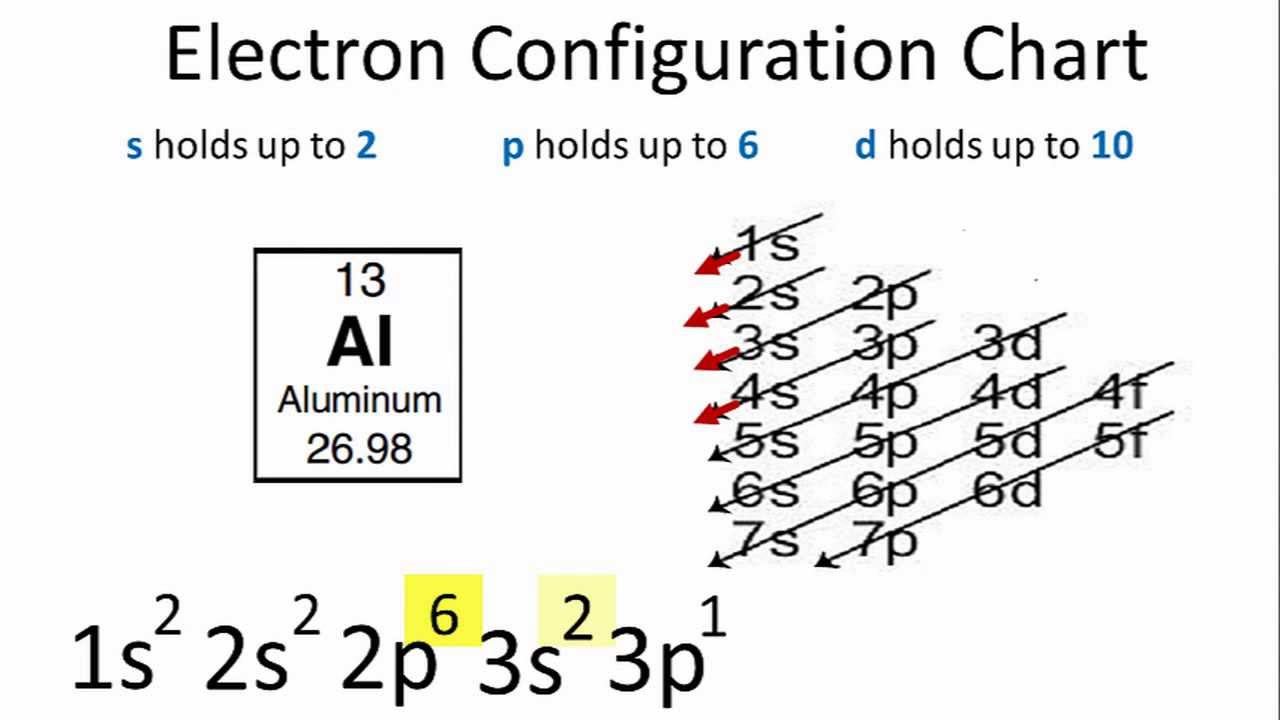
\includegraphics[width=\linewidth]{pic/econfig.jpg}

\end{minipage}%
\hspace{0.02\linewidth}
\begin{minipage}[t]{.50\linewidth}
\vspace{0pt}

\begin{center}
\begin{tabular}{cccc}
n & l & m & s\\
Haupt- & Neben- & Magnet- & Spin- \\
$1, 2, ...$ & $0, ..., n-1$ & $-l, ..., l$& $\pm \frac{1}{2}$\\
Schale & Orbital & Orientierung & Spinrichtung\\
K, L, M, ... & s, p, d, f & x, y z & up/down\\
\end{tabular}
\end{center}
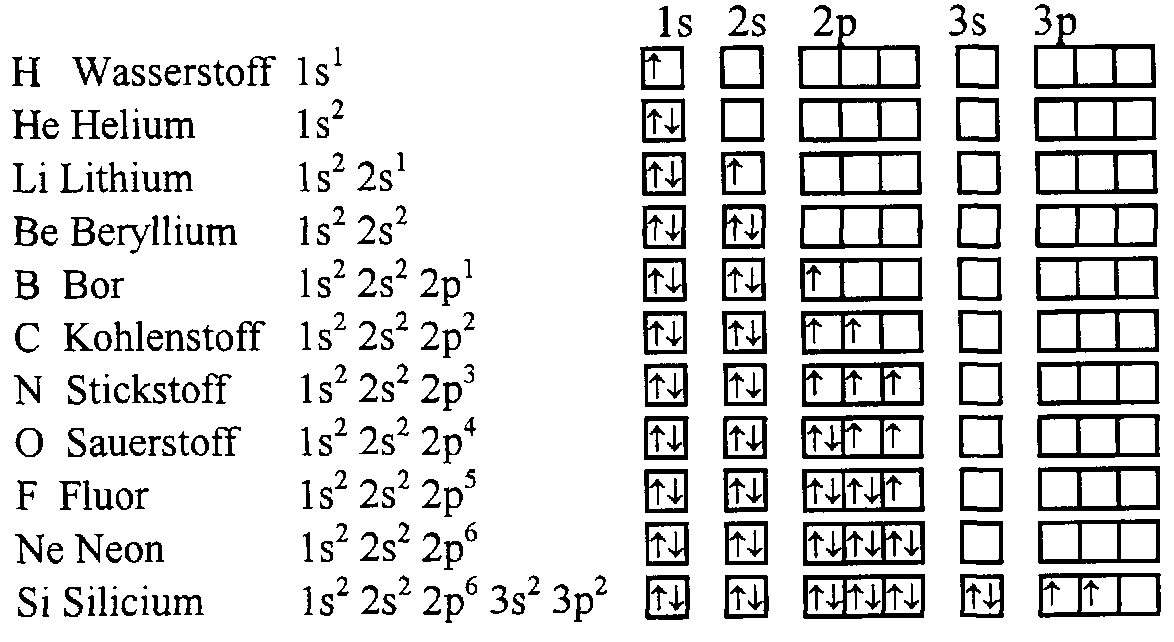
\includegraphics[width=\linewidth]{pic/kaestchen.png}

\end{minipage}
\end{center}

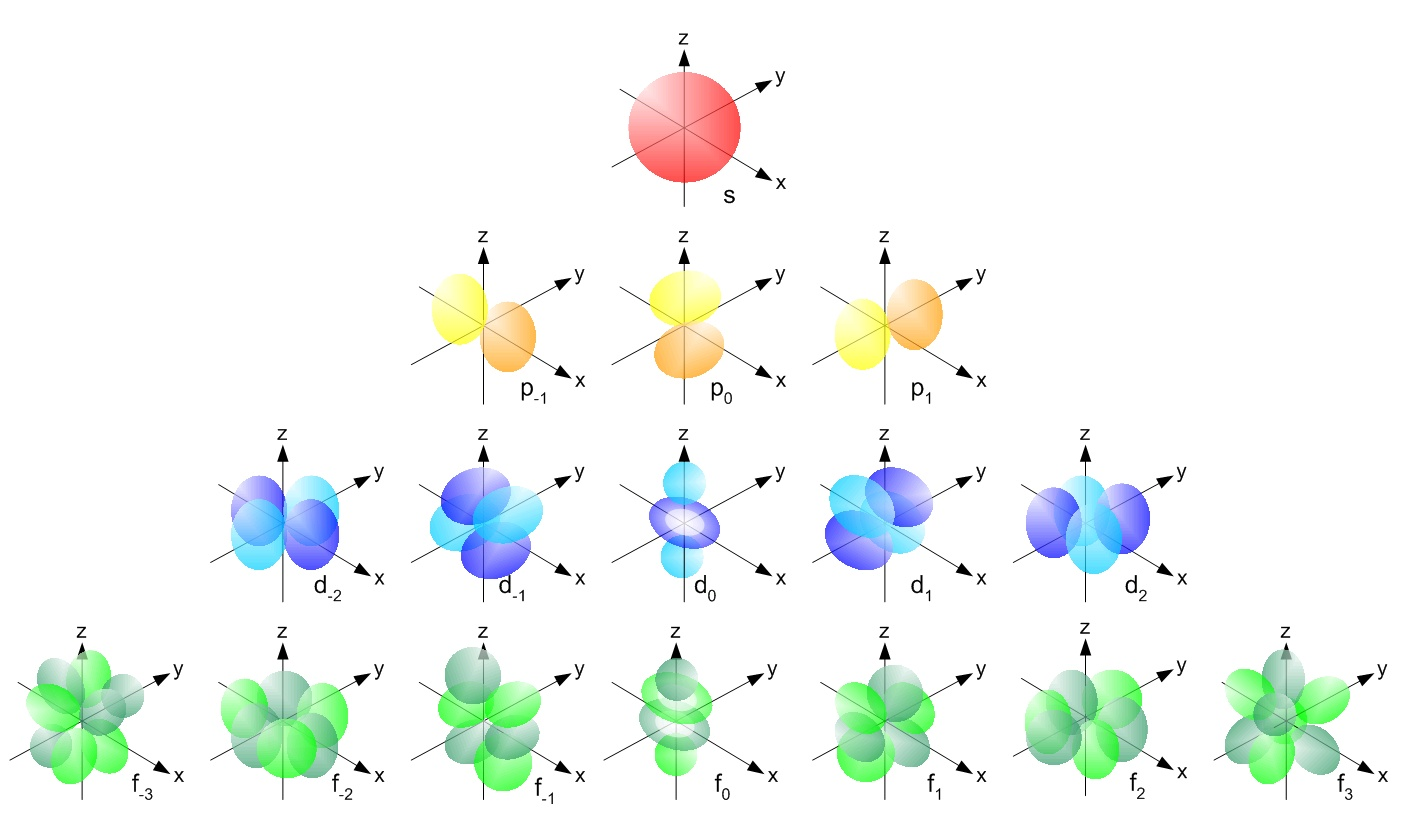
\includegraphics[width=\textwidth]{pic/orbitals.jpg}

\newpage

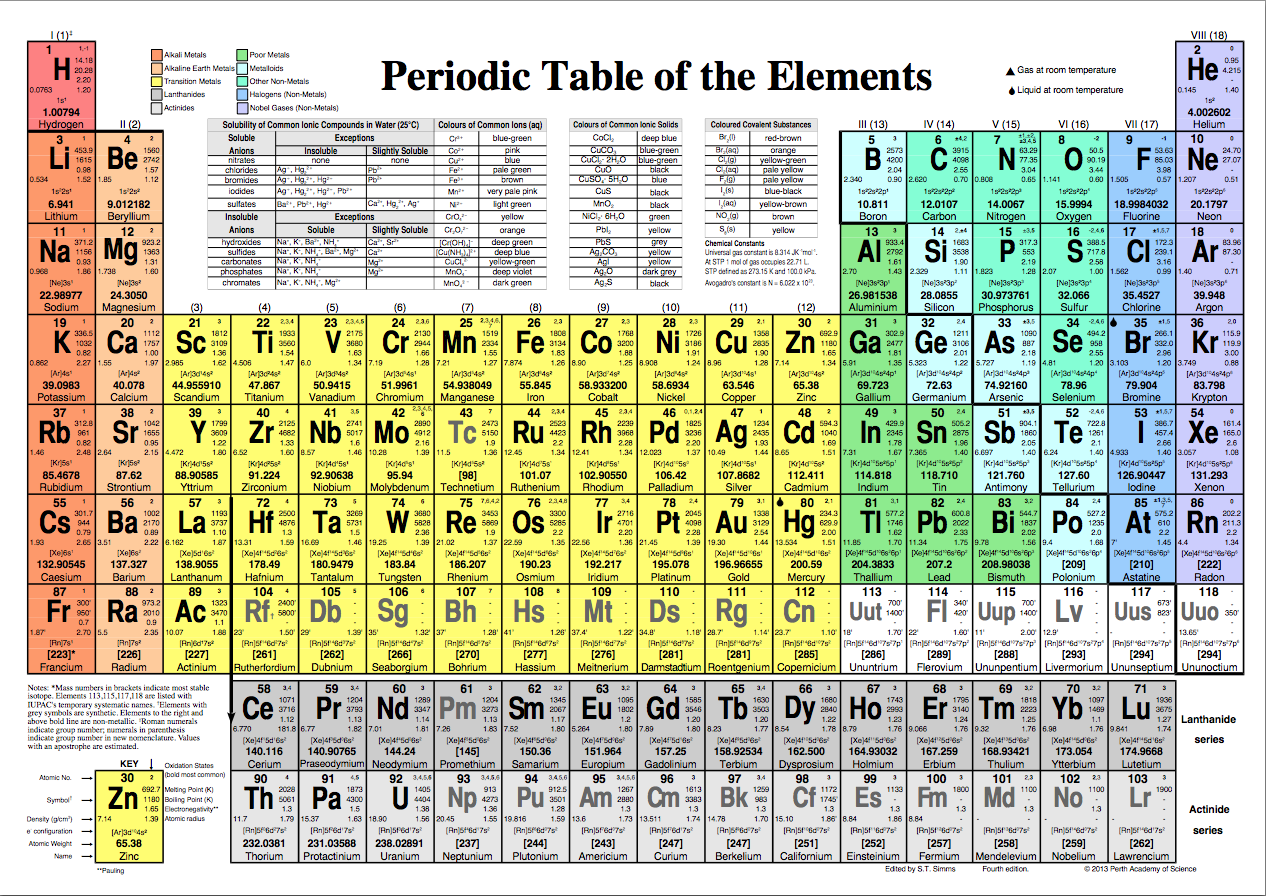
\includegraphics[width=0.9\textheight, angle=90]{pic/pse.png}
\newpage

\subsection{Stöchiometrie}

\begin{center}
\begin{minipage}[t]{.45\linewidth}
\vspace{0pt}

\begin{framed}
$$m_{Edukte} = m_{Produkte}$$
\begin{center}
\textsc{Gesetz von der Erhaltung der Masse}
\end{center}
\end{framed}

\begin{framed}
Elemente in einer chemische Verbindung kommen immer im gleichen konstanten Masseverhältnis vor.
\begin{center}
\textsc{Gesetz der konstanten Proportionen}
\end{center}
\end{framed}

\begin{framed}
Die Massenanteile der Elemente in allen chemischen Verbindungen gleicher Elemente stehen in einem ganzzahligen Verhältnis.
\begin{center}
\textsc{Gesetz der multiplen Proportionen}
\end{center}
\end{framed}

\end{minipage}%
\hspace{0.02\linewidth}
\begin{minipage}[t]{.45\linewidth}
\vspace{0pt}

Molare Masse: $m[g] = n[mol] \cdot M[g/mol]$\\
$N_A = 6,02217 \cdot 10^{23} =$ N in 12g $^{12}$C\\
amu: 1u $= 1,6606 \cdot 10^{-24}$g = $\frac{1}{12} m(^{12}$C)\\
Atommasse: $M = m_A N_A$\\

\begin{tabular}{ll}
Massenkonz. & $\beta(X)[g/l] = \frac{m(X)[g]}{V[l]}$\\
Vol.konz. & $\sigma(X)[ml/l] = \frac{V(X)[ml]}{V[l]}$\\
Stoffmengenkonz. & $c(X)[mol/l] = \frac{n(X)[mol]}{V[l]}$\\
\end{tabular}

\begin{tabular}{c|c|c}
Eigenschaft & Periode $\leftrightarrow$ & Gruppe $\updownarrow$\\
\hline
Atomradius & $\uparrow$ & $\downarrow$\\
Ionisierungsenergie & $\downarrow$ & $\uparrow$\\
Elektronenaffinität & $\downarrow$ & $\uparrow$\\
Elektronegativität & $\downarrow$ & $\uparrow$\\
Metallcharakter & $\downarrow$& $\uparrow$
\end{tabular}

\end{minipage}
\end{center}


\subsection{Kristalle}

\begin{framed}
\noindent \textbf{Ionenkristalle}:\\
\begin{tabularx}{\textwidth}{X|XXX}
 & CsCl-Typ & NaCl-Typ & ZnS-Typ\\
\hline
r$^+$/r$^-$ & $> 0,73$ & $0,73 - 0,41$ & $< 0,41$\\
Koordinationszahl & 8 & 6 & 4\\
Anordnung & kubisch & oktaedrisch & tetraedrisch
\end{tabularx}
\end{framed}
\begin{framed}
\noindent \textbf{Metallkristalle}:\\
\begin{tabularx}{\textwidth}{X|XXX}
 & Mg-Typ & Cu-Typ & W-Typ\\
\hline
Koordinationszahl & 12 & 12 & 8\\
Kugelpackung & hexagonal-dicht & kubisch-dicht & kubisch-raumzentriert\\
Raumausfüllung & 74\% & 74\% & 68\%\\
Beispiele & Mg, Ti, Co, Zn & Cu, Ni, Al, Ag & W, Na, Cr, Fe
\end{tabularx}
\end{framed}

\subsection{Chemische Thermodynamik}

\begin{center}
\begin{minipage}[t]{.5\linewidth}
\vspace{0pt}

\begin{framed}
\centering Die Enthalpieänderung ist vom Reaktionsweg unabhängig.
\begin{center}
\textsc{Gesetz von Hess}
\end{center}
\end{framed}

\begin{tabular}{ll}
Enthalpie & $\Delta H^{\circ}_{R} = \sum n_{P} \Delta H^{\circ}_{f, P} - \sum n_{E} \Delta H^{\circ}_{f, E}$\\
Entropie & $\Delta S^{\circ}_{R} = \sum n_{P} \Delta S^{\circ}_{P} - \sum n_{E} \Delta S^{\circ}_{E}$\\
Freie Energie & $\Delta G^{\circ}_{R} = \sum n_{P} \Delta G^{\circ}_{f, P} - \sum n_{E} \Delta G^{\circ}_{f, E}$
\end{tabular}

\end{minipage}%
\hspace{0.02\linewidth}
\begin{minipage}[t]{.4\linewidth}
\vspace{0pt}

\begin{framed}
$$\Delta G = \Delta H - T \Delta S$$
\begin{center}
\textsc{Gibbs-Helmholtz-Gleichung}
\end{center}
\end{framed}

endotherme Reaktion, $\Delta H > 0$\\
exotherme Reaktion, $\Delta H < 0$\\

\begin{tabular}{l|cc}
 & $\Delta H > 0$ & $\Delta H < 0$\\
\hline
$\Delta S > 0$ & spontan bei T$\uparrow$ & immer spontan\\
$\Delta S < 0$ & nie spontan & spontan T$\downarrow$
\end{tabular}

\end{minipage}
\end{center}


\subsection{Gasgesetze}

\begin{center}
\begin{minipage}[t]{.45\linewidth}
\vspace{0pt}

\begin{framed}
$$pV = nRT$$
\begin{center}
\textsc{Ideale Gasgleichung}
\end{center}
\end{framed}

\begin{framed}
$$V/T = const$$
\begin{center}
\textsc{Gesetz von Charles}
\end{center}
\end{framed}

\end{minipage}%
\hspace{0.02\linewidth}
\begin{minipage}[t]{.45\linewidth}
\vspace{0pt}

\begin{framed}
$$p/T = const$$
\begin{center}
\textsc{Gesetz von Gay-Lussac}
\end{center}
\end{framed}


\begin{framed}
$$n/V = const$$
\begin{center}
\textsc{Gesetz von Avogadro}
\end{center}
\end{framed}

\end{minipage}
\end{center}



\subsection{Lösung}

\begin{center}
\begin{minipage}[t]{.45\linewidth}
\vspace{0pt}

\begin{framed}
$$p = k_H c_l$$
\begin{center}
\textsc{Gesetz von Henry}\\
{\scriptsize $p$: Partialdruck Substanz, $c_l$: Konz. der Lösung}
\end{center}
\end{framed}

\end{minipage}%
\hspace{0.02\linewidth}
\begin{minipage}[t]{.45\linewidth}
\vspace{0pt}

\begin{tabular}{l|l}
Molarität & $\frac{n(X)[mol]}{V(\text{Lösung})[l]}$\\[11pt]
Molalität & $\frac{n(X)[mol]}{m(\text{Lösungsmittel})[kg]}$\\[11pt]
Massenprozent & $\frac{m(X)[kg]}{m(\text{Lösung})[kg]} \cdot 100\%$
\end{tabular}

\end{minipage}
\end{center}

\subsection{Reaktionskinetik}

\begin{center}
\begin{minipage}[t]{.45\linewidth}
\vspace{0pt}

\begin{framed}
$$K_C = \frac{c_C^{\nu(C)} \cdot c_D^{\nu(D)}}{c_A^{\nu(A)} \cdot c_B^{\nu(B)}}$$
\begin{center}
\textsc{Massenwirkungsgesetz}\\
\scriptsize{(Konzentrationen oder Partialdrücke)}\\
\scriptsize{für \ch{$\nu$ A + $\nu$ B <=> $\nu$ C + $\nu$ D}}
\end{center}
\end{framed}

$K>>1$: Gleichgewicht bei Produkten\\
$K=1$: Glgw. bei gleicher Konzentration\\
$K<<1$: Reaktion läuft nicht ab\\
Reaktionsgeschwindigkeit: $r = \frac{\Delta c}{\Delta t}$

\end{minipage}%
\hspace{0.02\linewidth}
\begin{minipage}[t]{.45\linewidth}
\vspace{0pt}

\begin{framed}
Übt man auf ein chemisches System im Gleichgewicht einen Zwang aus, so reagiert es so, dass die Wirkung des Zwanges minimal wird.
\begin{center}
\textsc{Prinzip von Le Châtelier}
\end{center}
\end{framed}

\begin{framed}
$$K = e^{-\frac{E_A}{RT}}$$
\begin{center}
\textsc{Arrhenius-Gleichung}\\
{\scriptsize $E_A$: Aktivierungsenergie}
\end{center}
\end{framed}

\end{minipage}
\end{center}


\subsection{Redox-Reaktionen}

\begin{enumerate}
\item Reaktionsgleichung aufstellen\\
$\ch{PbO2 + Mn\pch[2] -> MnO4\mch[] + Pb\pch[2]}$
\item Oxidationszahlen bestimmen\\
$\ch{\ox{4,Pb} \ox{-2,O} 2 + \ox{2,Mn} \pch[2] -> \ox{7,Mn} \ox{-2,O} 4\mch[] + \ox{2,Pb} \pch[2]} $
\item Herausfinden, welche Stoffe reduziert (Ox.zahlen nehmen ab) und welche oxidiert (Ox.zahlen nehmen zu) werden\\
$\ch{Mn\pch[2]}$ wird oxidiert (von +II auf +VII)\\
$\ch{PbO2}$ wird reduziert (von +IV auf +II)
\item Teilreaktionen formulieren\\
Oxidation: $\ch{"\ox{2,Mn}" \pch[2] -> "\ox{7,Mn}" "\ox{-2,O}" 4\mch[]}$\\
Reduktion:$ \ch{"\ox{4,Pb}" "\ox{-2,O}" 2 -> "\ox{2,Pb}" \pch[2]}$
\item Ladungsausgleich\\
$\ch{"\ox{2,Mn}" \pch[2] -> "\ox{7,Mn}" "\ox{-2,O}" 4\mch[] - 5 e\mch[]}$\\
$\ch{"\ox{4,Pb}" "\ox{-2,O}" 2 + 2 e\mch[] -> "\ox{2,Pb}" \pch[2]}$
\item Auf geeignetes Vielfaches bringen und addieren\\
$\ch{5 PbO2 + 2 Mn\pch[2] -> 2 MnO4\mch[] + 5 Pb\pch[2]}$
\begin{itemize}
	\item Saures Milieu: Auf der Seite mit zu wenig Sauerstoff Wasser addieren, auf der Seite mit zu wenig Wasserstoff Hydronium-Ionen (bzw. \Hpl ) addieren\\
	$\ch{5 PbO2 + 2 Mn\pch[2] + 4 \Hpl -> 2 MnO4\mch[] + 5 Pb\pch[2] + 2 H2O}$
	\item Basisches Milieu: genauso, aber am Schluss Hydroxid-Ionen (\Hyd) (auf beiden Seiten) addieren, um \Hpl zu neutralisieren.
\end{itemize}
\end{enumerate}

\subsection{Elektrochemie}

\begin{center}
\begin{minipage}[t]{.45\linewidth}
\vspace{0pt}

\begin{framed}
$$E = E_0 + \frac{0,059}{n} \log \frac{c(Ox)}{c(Red)}$$
\begin{center}
\textsc{Nernst'sche Gleichung}
\end{center}
\end{framed}

\end{minipage}%
\hspace{0.02\linewidth}
\begin{minipage}[t]{.45\linewidth}
\vspace{0pt}

\begin{framed}
$$m = \frac{Mq}{zF}$$
\begin{center}
\textsc{1. und 2. Faraday-Gesetz}\\
\scriptsize{mit F: Faraday-Konstante}
\end{center}
\end{framed}

\end{minipage}
\end{center}

\noindent
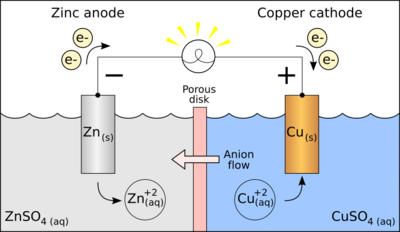
\includegraphics[width=\textwidth]{pic/galva2.png}

\newpage
\section{Konstanten, Abkürzungen, Einheiten und Eselsbrücken}

\subsection{Abkürzungen}

\begin{tabular}{ll}
hO & harmonischer Oszillator\\
sK & starrer Körper\\
CMS & center of mass system\\
iG & ideales Gas\\
bb & schwarzer Körper\\
mP & mathematisches Pendel\\

\end{tabular}

\subsection{Konstanten}
Lichtgeschwindigkeit \dotfill $c = 299 792 458 \frac{m}{s}$\\
Bohr'sches Magneton \dotfill $\mu_B = \frac{e\hbar}{2m_e} = 9,27 \times 10^{-24} J/T = 5,79 \times 10^{-5} eV/T$\\
Vakuumpermeabilität \dotfill $\mu_0 = 4\pi \times 10^{-7} \frac{Vs}{Am}$\\
Gasvolumen bei STP: $V = n V_m$ mit $V_m = 22,4$l/mol\\
$R = 8,314$ J/mol K


\subsection{Eselsbrücken}

$1eV = 8065,541 cm^{-1}$\\
$\hbar c = 197$ eVnm\\
$\lambda = \frac{12{\text \AA}}{\sqrt{U}}$\\
Erdmasse: $6 \cdot 10^{24} kg$\\
$h = 2 \pi \cdot 10^{-34} Js$, $\hbar = 10^{-34} Js$\\
thermische Energie Raumtemperatur: $300K = 25meV$\\
$k_B = \frac{25}{300} \cdot 10^{-3} \frac{eV}{K}$\\
$hc = 1240 eVnm$\\
$m_e = 9,11 \cdot 10^{-31}kg$\\
Sekunden pro Jahr: $\pi \cdot 10^7$\\
$m_p / m_e$: $2000$\\
$1 \frac{km}{s}  = \frac{parsec}{Ma}$\\
$m_p[g] = \frac{1}{N_A} = \frac{1}{6,022 \cdot 10^{23}}$


\subsection{Einheiten}



Drehimpuls: $kg \frac{m^2}{s} = Js$\\
\begin{tabular}{r|l||r|l}
W & $Nm$ & L & $kgm^2$\\
P & $J/s$ & $\varepsilon_0$ & $C^2/Nm^2$\\
$\varphi$ & $J/C$ & $\mu_0$ & $N/A^2$\\
B & $N/Am$ & R & $J/mol K$\\
$\Phi$ & $Tm^2$ & $k_B$ & $J/K$\\
L & $J/A^2$ & $\Gamma$ & $Nm^2/kg^2$\\
I & $W/m^2$ & &
\end{tabular}



\end{document}
